% This is a package nagging about deprecated stuff. We use
% RequirePackage instead of usepackage here because we want nagging
% for stuff that happens inside the \documentclass command.
% Note that currently (15.10.2012 16:12), nag has a bug with
% subcaption and complains about labels in a float before the caption.
\RequirePackage[l2tabu,orthodox]{nag}

\documentclass[ngerman,a4paper,11pt]{article}

% This (I mean [gray]) makes the minted source code grayscale. Has to
% be at the top here because other packages include xcolor, too
\usepackage[gray]{xcolor}

% This losely emulates the old \usepackage{a4wide}.
\usepackage{geometry}
\geometry{
  includeheadfoot,
  margin=2.8cm
}

% Packages
% This has to do with German Umlauts in pdf documents
\usepackage[T1]{fontenc}
% File encoding
\usepackage[utf8]{inputenc}
% Hyphenation, internationalization of labels.
\usepackage[ngerman]{babel}
% For \begin{align}
\usepackage{amsmath}
% For theorems
\usepackage{amsthm}
% For \mathbb
\usepackage{amssymb}
% Hopefully produces less noisy output
\usepackage{silence}
% For internationalized quotes (of all kinds)
\usepackage{csquotes}
% For subfigures and figures (alle)
\usepackage{graphicx}
\usepackage[footnotesize,bf]{caption}
\usepackage[subrefformat=parens,labelformat=parens]{subcaption}
% For pdf Links. The pdfborder removes the box around links
\usepackage[pdfborder={0 0 0},breaklinks=true]{hyperref}

% Beide für Tabellen
\usepackage{array}
\usepackage{booktabs}

% Pseudocode
\usepackage{algorithmicx}
\usepackage{algorithm}
\usepackage{algpseudocode}

% Für URLs in Bibliografie
\usepackage{url}
\usepackage{breakurl}

\usepackage{minted}

% Macros
\newcommand{\PimiddyName}[1]{\emph{#1}}
% Abbreviations need special care when it comes to whitespace both
% inbetween the letters and at the end. The macros below wrap the most
% common abbreviations.
\newcommand{\PimiddyzB}{z.\,B.\ }
\newcommand{\Pimiddydh}{d.\,h.\ }
\newcommand{\Pimiddyvgl}{vgl.\ }
\newcommand{\Pimiddyengl}{engl.\ }
\newcommand{\Pimiddyetal}{et.\ al.\ }
\newcommand{\Pimiddyggf}{ggf.\ }
\newcommand{\Pimiddybzw}{bzw.\ }
\newcommand{\Pimiddyca}{ca.\ }

% Other Macros
\newcommand{\PimiddyBegriff}[1]{\textbf{#1}}
\newcommand{\PimiddyBetrag}[1]{\left|#1\right|}
\newcommand{\PimiddyEnglBegriff}[1]{#1}
\newcommand{\PimiddyQuotes}[1]{\enquote{#1}}
\newcommand{\PimiddyFormelText}[1]{\textnormal{#1}}
\newcommand{\PimiddyAufrunden}[1]{\lceil{} #1 \rceil{}}
\newcommand{\PimiddyReell}{\ensuremath{\mathbb{R}}}
\newcommand{\PimiddyGanz}{\ensuremath{\mathbb{Z}}}
\newcommand{\PimiddyNorm}[2]{\left\|#2\right\|_{#1}}
\newcommand{\PimiddyFootnote}[1]{\footnote{#1}}
\newcommand{\PimiddyTodo}[1]{{\footnote{\textbf{TODO\@: #1}}}}
\newcommand{\PimiddyEnglisch}[1]{{engl. \emph{#1}}}
\newcommand{\PimiddyTableHeading}[1]{{\textbf{#1}}}
\newcommand{\PimiddyInlineCode}[1]{{\texttt{#1}}}
\newcommand{\PimiddyModulo}{\bmod}
\newcommand{\PimiddyDegree}[1]{\ensuremath{{#1}^{\circ}C}}

\numberwithin{figure}{section}
\numberwithin{equation}{section}
\numberwithin{table}{section}
\numberwithin{algorithm}{section}

% Operators
\DeclareMathOperator*{\PimiddyGrad}{grad}
\DeclareMathOperator*{\PimiddyDiv}{div}
\DeclareMathOperator*{\PimiddyRot}{rot}
\newcommand{\PimiddyLaplace}{\Delta}
\newcommand{\PimiddyProjection}{\mathbb{P}}
\DeclareMathOperator*{\PimiddyVectorfields}{Vect}
\DeclareMathOperator*{\PimiddyScalarfields}{Scal}

% Theorems
\newtheorem*{PimiddySatz}{Satz}

% For latex+inkscape to work. The eps_tex files use \includegraphics{foo.eps}
% which diesn't find the images unless this is defined
\graphicspath{{images/}}
% Also for latex+inkscape
% Also for general colors, dvipsnames adds more colors
%\usepackage[usenames,dvipsnames]{xcolor}

\usepackage{listings}

% Fette Monospacefonts
% bold-extra funzt irgendwie nicht
%\usepackage{bold-extra}
%\usepackage[scale=0.9]{beramono}
\usepackage{pxfonts}

%\includeonly{stam}

\usepackage[nameinlink]{cleveref}

% With this, we can use @online to cite websites in a bibtex file
\usepackage[backend=bibtex]{biblatex}

\bibliography{mendeley_bibliography,other_sources}
\begin{document}
\tableofcontents
\section{Danksagungen}

Hiermit möchte ich allen Personen danken, die mich bei der Erstellung der Arbeit
unterstützt haben:

\begin{itemize}
\item Herrn Prof. Dr. Oliver Vornberger für die Tätigkeit als Erstgutachter und
für die Bereitstellung der interessanten Thematik.
\item Frau Prof. Dr. Sigrid Knust, die sich als Zweitgutachterin zur Verfügung gestellt hat.
\item Frau Jana Lehnfeld und Herrn Henning Wenke für das wertvolle Feedback
während der Verfassung der Arbeit.
\end{itemize}

\section{Zusammenfassung}

Die vorliegende Arbeit entstand in der Arbeitsgruppe Medieninformatik an der Universität Osna
im Bereich Computergrafik und beschäftigt sich mit prozeduraler Modellierung. Kern
der Arbeit ist die Generierung einer Schneedecke, um Wetterverhältnisse anhand
von Wetterdaten naturgetreu darstellen zu können. Dazu wird der Anzatz einer
Repräsentation durch Voxel in einem regelmaßigen Voxelgitter verfolgt. Für die
realistische Verteilung des Schnees sorgt dabei die Simulation zufalligen
Schneefalls sowie ein Stabilitatstest, der die Entstehung unnaturlich hoher
Schneeturme verhindert. Abschließend wird das Voxelgitter unter Verwendung des
sogenannten Marching-Cubes-Algorithmus’ in eine schneeahnliche Oberflache
uberfuhrt.

\section{Einleitung}

Die Arbeit befasst sich mit der Modellierung und Entwicklung einer Methode zur
Simulation von Wind, sowie einem Partikelsystem für Schneeflocken. Zu Anfang
soll ein Überblick über die Zielsetzung gegeben werden. Danach folgt eine kurze
Zusammenfassung vorhandener Simulationsmethoden. Hier wird die Entscheidung für
eine der Methoden begründet vorgestellt. Schließlich folgt ein Überblick über
den Aufbau der Arbeit.

\subsection{Motivation}

...

\subsection{Zielsetzung}

...

\subsection{Aufbau}

Obacht, was folgt ist aus dem eigentlich geplanten Kapitel
``Implementierung'' entnommen, daher fehlt noch was am Grundaufbau.

In diesem Kapitel soll auf die Details der Implementierung eingegangen werden. Es
wird zunächst OpenGL eingeführt, was zur Visualisierung eingesetzt wird. Danach
wird OpenCL eingeführt, was für die eigentlichen Berechnungen zuständig ist.

Danach das Verfahren von Stam mittels OpenCL umgesetzt. Als Ausgabe erhält man
ein Schnee-Vektorfeld, was dann weiterverwendet werden kann. Hier wird auch auf
Hindernisse wie Gebäude eingegangen. Dazu gehört das Laden der Hindernisse aus
obj-Dateien sowie die Anzeige mittels OpenGL, sowie die Einspeisung in die
Simulation.

Anschließend wird der fallende Schnee modelliert. Hierzu soll zunächst die
Entstehung von Schnee in der Natur erläutert werden, sowie physikalische
Hindergründe bezüglich fallendem Schnee.

Diese idealen physikalischen Gegebenheiten werden dann in ein einfacheres
Modell transformiert, welches für das Partikelsystem verwendet wird. Zu diesem
Partikelsystem gehört neben der Simulation auch die Visualisierung, für die in
dieser Arbeit Pointsprites verwendet werden.

Im letzten Abschnitt wird schließlich auf die Modellierung der Schneedecke
eingegangen, wobei die Ergebnisse von Manuel Schwarz \cite{Schwarz2012} eine
tragende Rolle spielen. Außerdem werden noch einige weitere
Anwendungsmöglichkeiten der Fluidsimulation wie die Simulation von Rauch
angesprochen.

\section{Mathematische Grundlagen}
\label{sec:mathematics}

Die Berechnungen in dieser Arbeit finden alle im reellen Raum statt, also in den
Vektorräumen $\PimiddyReell^n, n \in \{1,2,3\}$. Die Gleichungen der
Strömungsmechanik benutzen \PimiddyBegriff{Vektorfelder} und
\PimiddyBegriff{Skalarfelder}, daher werden diese Begriffe und die zugehörigen
Operationen zunächst eingeführt.

Die später betrachteten Gleichungen sind allerdings meist gar nicht oder nur sehr
schwer analytisch zu lösen, daher greift man auf numerische Verfahren zurück.
Dafür ist es notwendig, Operationen wie den Gradienten oder die
Divergenz zu \emph{diskretisieren}. Im letzten Teil des Abschnitts
werden verschiedene Arten der Diskretisierung erläutert.

\subsection{Kontinuierliche Felder}

Für eine Funktion $f \colon \PimiddyReell^n \to \PimiddyReell$ bezeichne

\begin{equation}
\frac{\partial f}{\partial x_i}
\end{equation}

die \PimiddyBegriff{partielle Ableitung} nach der $i$-ten Komponente.

Ein \PimiddyBegriff{Vektorfeld} $\vec{u}$ ist eine Abbildung

\begin{equation*}
\vec{u} \colon \PimiddyReell^n \to \PimiddyReell^n,
\end{equation*}

die einem Punkt im Raum einen Pfeil zuordnet. So kann \PimiddyzB{}jedem
Punkt im Raum die Windgeschwindigkeit an diesem Punkt zugeordnet
werden. \autoref{fig:mathematics_vectorfield} zeigt ein solches
Vektorfeld.

$\PimiddyVectorfields(\PimiddyReell^n)$ bezeichne die Menge aller
Vektorfelder. In dieser Arbeit betrachtete Vektorfelder sind stets
differenzierbar.

Analog ist ein \PimiddyBegriff{Skalarfeld} $p$ eine Abbildung

\begin{equation*}
p \colon \PimiddyReell^n \to \PimiddyReell
\end{equation*}

welche einem Punkt im Raum einen skalaren Wert zuordnet. Beispielsweise könnte
für jeden Punkt im Raum die dortige Temperatur in einem Skalarfeld gespeichert
sein (siehe \autoref{fig:mathematics_scalarfield}).
$\PimiddyScalarfields(\PimiddyReell^n)$ bezeichne die Menge aller
Skalarfelder. Auch alle Skalarfelder sind in dieser Arbeit
differenzierbar.

\begin{figure}
	\begin{subfigure}[t]{0.5\textwidth}
		\centering
		
\includegraphics[width=\textwidth]{images/vectorfield}
		\caption{Ein Vektorfeld}
		\label{fig:mathematics_vectorfield}
	\end{subfigure}
	~
	\begin{subfigure}[t]{0.5\textwidth}
		\centering
		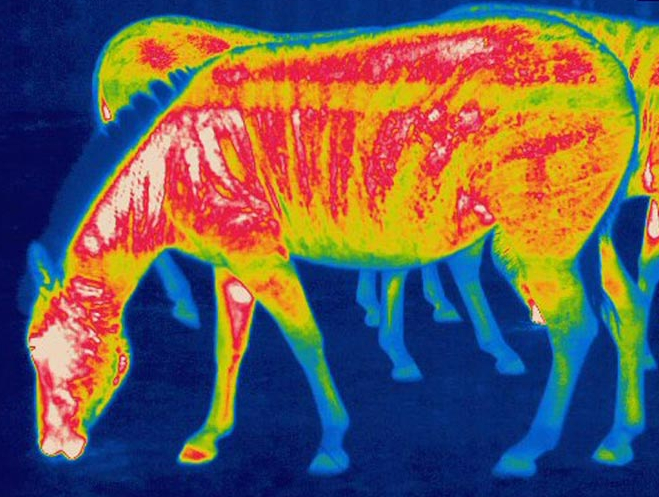
\includegraphics[width=\textwidth]{images/thermal_imaging}
		\caption{Die Körpertemperatur eines Pferds als Skalarfeld.}
		\label{fig:mathematics_scalarfield}
	\end{subfigure}
	\caption{Die betrachteten Feldtypen}
\end{figure}

Sei $p$ ein dreidimensionales Skalarfeld, dann ist der \PimiddyBegriff{Gradient}
$\PimiddyGrad p$ definiert als:

\begin{equation}
\begin{aligned}
\PimiddyGrad \colon \PimiddyScalarfields \to \PimiddyVectorfields \\
\PimiddyGrad p
=
\left( \frac{\partial p}{\partial x},\frac{\partial p}{\partial y},\frac{\partial p}{\partial z} \right)
\end{aligned}
\end{equation}

\begin{figure}[ht]
        \captionsetup{singlelinecheck=off}
	\begin{subfigure}[t]{0.5\textwidth}
		\centering
		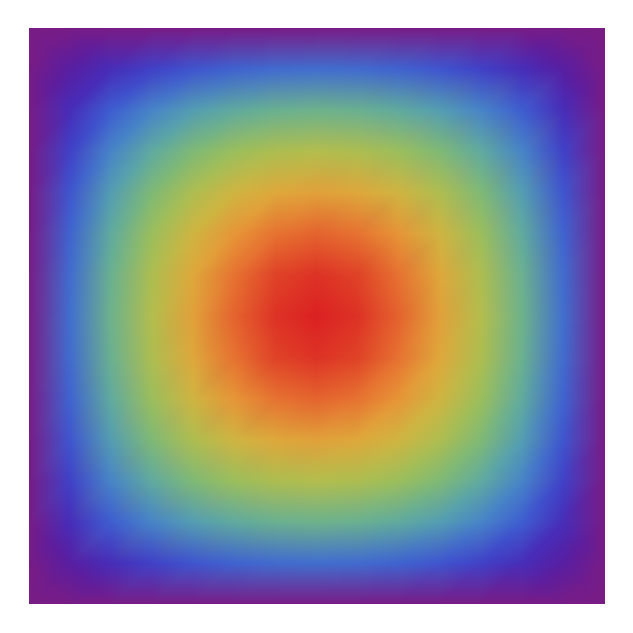
\includegraphics[width=\textwidth]{images/scalar_field_to_show_gradient}
		\caption{Das Skalarfeld zur Funktion \[ f(x,y) = \sin(x)\sin(y) \] Rötliche Färbung deutet hohe Werte an, lila und blau geringe.}
		\label{fig:mathematics_sample_scalar_field}
	\end{subfigure}
	~
	\begin{subfigure}[t]{0.5\textwidth}
		\centering
		
\includegraphics[width=\textwidth]{images/gradient_of_scalar_field}
		\caption{Der Gradient des Skalarfeldes \[ f(x,y)=(\sin(y)\cos(x),\sin(x)\cos(y)) \]}
		\label{fig:mathematics_gradient_of_sample_scalar_field}
	\end{subfigure}
	\caption{Der Gradient am Beispiel}
	\label{fig:mathematics_gradient_of_sample_scalar_field_total}
\end{figure}

Der Gradient eines Skalarfeldes ist also ein Vektorfeld, nämlich das
Vektorfeld der partiellen Ableitungen. Genauso wie die Ableitung eines
Graphen die Steigung an jedem Punkt angibt, so zeigt der Gradient
eines Feldes in die Richtung des steilsten Anstiegs. Die Länge des
Gradienten gibt die Größe der Steigung in diesem Punkt an. Der
Gradient des negativen Skalarfeldes $-p$ zeigt folglich in Richtung
des größten Gefälles.
\autoref{fig:mathematics_gradient_of_sample_scalar_field_total} zeigt
ein simples Beispiel für den Gradienten.

Für differenzierbare Vektorfelder $\vec{u}$ ist die
\PimiddyBegriff{Divergenz} auf dem Feld definiert als

\begin{equation}
\begin{aligned}
\PimiddyDiv \colon \PimiddyVectorfields \to \PimiddyScalarfields \\
\PimiddyDiv \vec{u}
=
\frac{\partial u^x}{\partial x} +
\frac{\partial u^y}{\partial y} +
\frac{\partial u^z}{\partial z}
\end{aligned}
\end{equation}

Hier sind $u^x,u^y,u^z$ die einzelnen Komponenten des Vektorfelds. Die
Divergenz eines Vektorfelds ist also ein Skalarfeld. Dieses Skalarfeld kann
gedeutet werden als \PimiddyQuotes{Quellendichte} des ursprünglichen
Vektorfelds\PimiddyTodo{Hier muss noch ein Bild hin.}. Ein Feld
$\vec{u}$, welches $\PimiddyDiv \vec{u}=0$ erfüllt, heißt folglich
\PimiddyBegriff{quellenfrei}.

In der Physik findet man den Gradienten und die Divergenz meist unter dem Symbol
$\nabla$ vereint. Je nachdem, ob es auf ein Vektor- oder ein Skalarfeld
angewendet wird, wechselt es die Bedeutung.
%Diese Notation wird in der Arbeit bevorzugt, da man die Symbole $\PimiddyGrad$ bzw.\ $\PimiddyDiv$ in der Literatur zu Fluiddynamik kaum vorfindet.

Auf Vektorfeldern ist schließlich die \PimiddyBegriff{Rotation}
definiert als:

\begin{equation}
\begin{aligned}
\PimiddyRot \colon \PimiddyVectorfields \to \PimiddyVectorfields \\
\PimiddyRot \vec{u}
=
\left(
	\begin{array}{c}
		\frac{\partial u^z}{\partial y} - \frac{\partial u^y}{\partial z} \\
		\frac{\partial u^x}{\partial z} - \frac{\partial u^z}{\partial x} \\
		\frac{\partial u^y}{\partial x} - \frac{\partial u^x}{\partial y}
	\end{array}
\right)
\end{aligned}
\end{equation}

Wie der Name schon andeutet gibt sie für jeden Punkt des
ursprünglichen Vektorfelds an, wie stark und in welche Richtung das
Feld in diesem Punkt rotiert. Im Zweidimensionalen ist die Rotation
auch definiert, hier ergibt sich für jeden Punkt im Raum allerdings
nur ein Skalar, kein Vektor. Die Rotationsachse ist immer die
imaginäre \PimiddyQuotes{$z$-Achse} (in
\autoref{fig:mathematics_scalarfield} wäre die Rotation überall
konstant). Ein Feld $\vec{u}$, welches $\PimiddyRot \vec{u}=0$
erfüllt, heißt \PimiddyBegriff{rotationsfrei}.

\begin{figure}
	\begin{subfigure}[b]{0.5\textwidth}
		\centering
		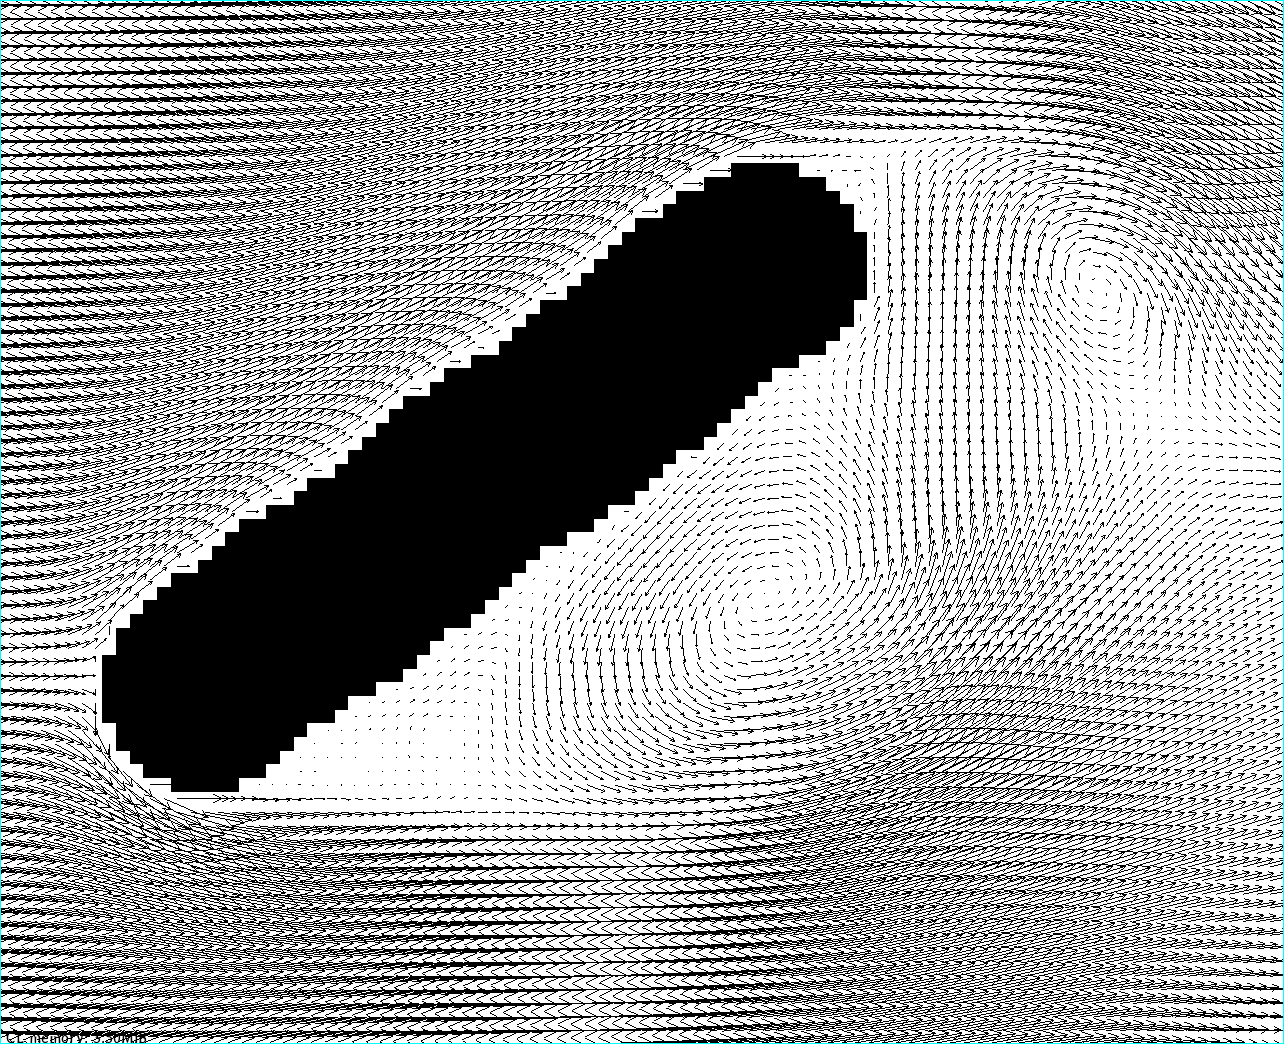
\includegraphics[width=\textwidth]{images/vector_field_rotation_arrows}
		\label{fig:mathematics_image_vectorfield_rotation_arrows}
	\end{subfigure}
	~
	\begin{subfigure}[b]{0.5\textwidth}
		\centering
		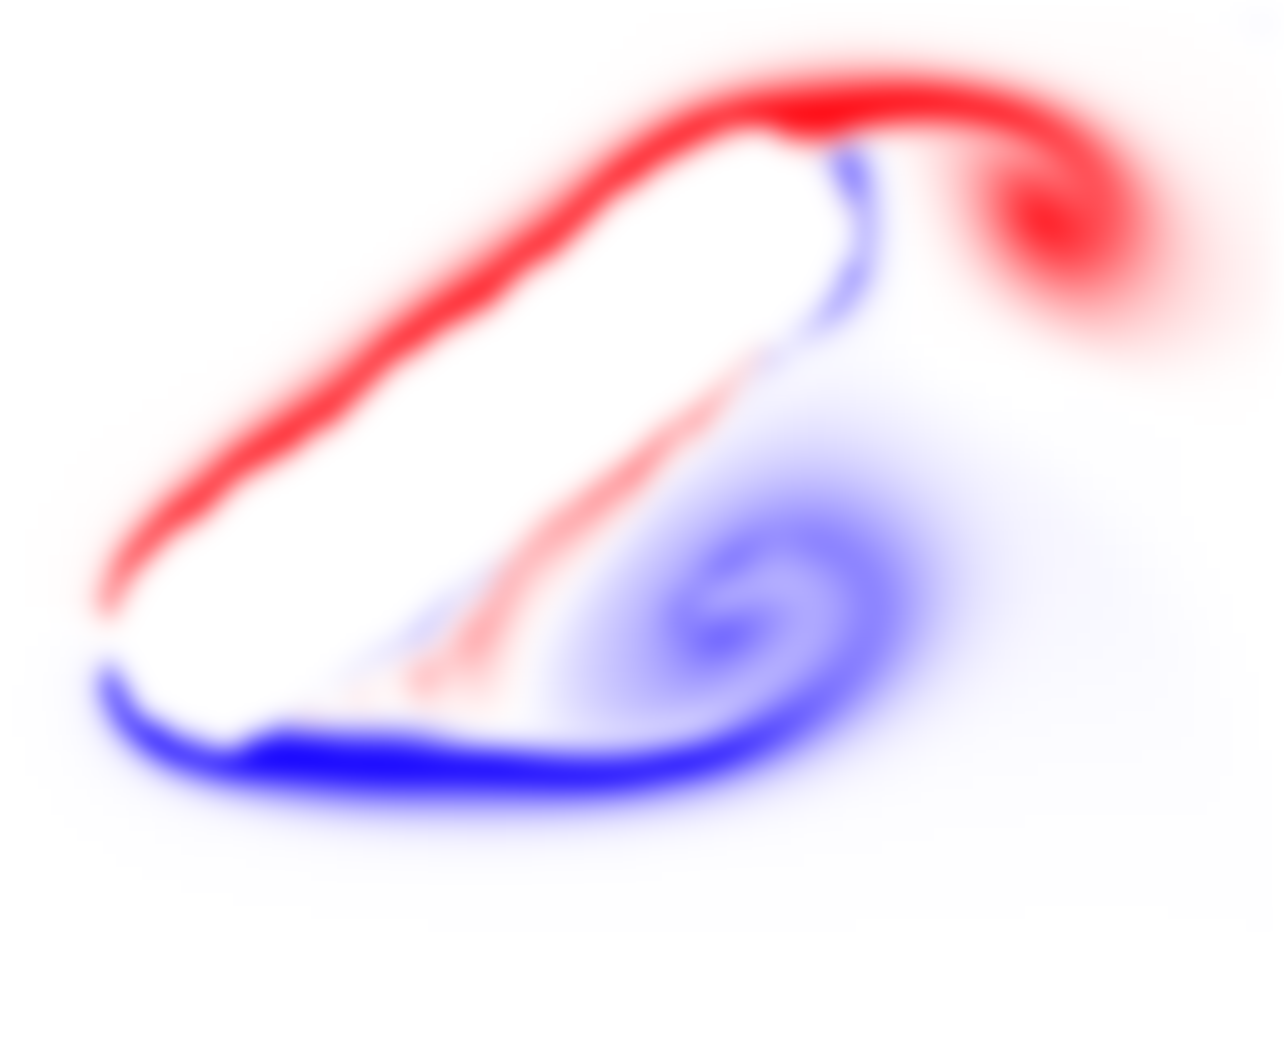
\includegraphics[width=\textwidth]{images/vector_field_rotation}
	\end{subfigure}
	\caption{Ein 2D-Strömungsfeld, das um ein Hindernis herumfließt mit dazugehöriger Rotation. Negative Rotation ist rot gekennzeichnet, positive in blau.}
\end{figure}

Schaltet man $\PimiddyGrad$ und $\PimiddyDiv$ hintereinander, erhält man den
\PimiddyBegriff{Laplace-Operator}:

\begin{equation}
\begin{aligned}
\PimiddyLaplace \colon \PimiddyScalarfields \to \PimiddyScalarfields \\
\PimiddyLaplace p = \PimiddyDiv \PimiddyGrad p
\end{aligned}
\end{equation}

Manchmal wird auch das Symbol $\nabla^2$ für den Laplace-Operator benutzt. Im Dreidimensionalen ergibt sich:

\begin{equation}
\PimiddyLaplace p =
\frac{\partial^2 p}{\partial^2 x} +
\frac{\partial^2 p}{\partial^2 y} +
\frac{\partial^2 p}{\partial^2 z}
\end{equation}

Intuitiv misst der Operator für jeden Punkt $\vec{x}$ die Abweichung von
$p(\vec{x})$ zu Punkten in seiner Umgebung. Die diskretisierte Variante dieses
Operators wird deswegen in der Bildverarbeitung zum Erkennen von Kanten in
Bildern verwendet (siehe \autoref{fig:mathematics_image_laplacian}).

\begin{figure}[ht]
	\begin{subfigure}[t]{0.5\textwidth}
		\centering
		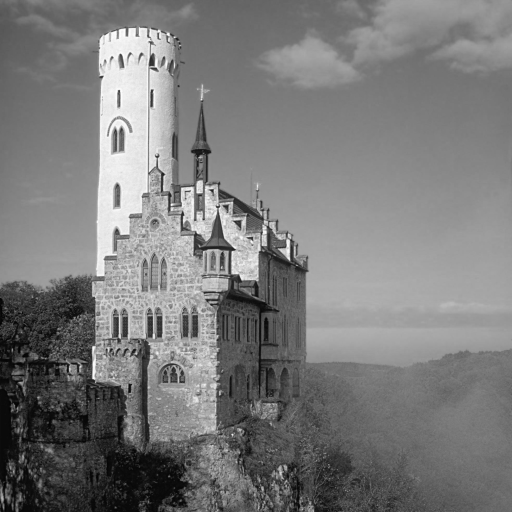
\includegraphics[width=\textwidth]{images/schloss_grey}
		\caption{Originalbild}
	\end{subfigure}
	~
	\begin{subfigure}[t]{0.5\textwidth}
		\centering
		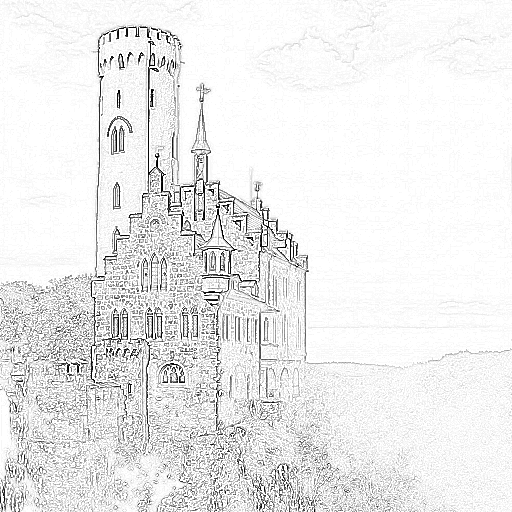
\includegraphics[width=\textwidth]{images/schloss_grey_laplace}
		\caption{Das Bild nach Anwendung des Laplace-Operators}
		\label{fig:mathematics_image_laplacian}
	\end{subfigure}
\end{figure}


Der Operator lässt sich auf nahe liegende Weise auf Vektorfelder erweitern, in drei Dimensionen
ergibt sich:

\begin{equation}
\PimiddyLaplace \vec{u} =
\left(
	\begin{array}{c}
		\PimiddyLaplace u^x \\
		\PimiddyLaplace u^y \\
		\PimiddyLaplace u^z
	\end{array}
\right)
\end{equation}

\subsection{Diskretisierung}
\label{sec:mathematics_discretization}

Die eben vorgestellten mathematischen Definitionen gehen vom
unendlichen, kontinuierlichen Raum $\PimiddyReell^n$ aus. Für die
Berechnungen wird aber ein endliches, diskretes Gitter verwendet, also
eine Teilmenge von $\PimiddyGanz^n$. Eine Zelle in dem diskreten
Gitter wird auch \PimiddyBegriff{Voxel} (für
\PimiddyQuotes{Volumen-Pixel}) genannt. Die eben vorgestellten
Operatoren müssen in eine diskrete Form gebracht werden. Dies wird
hier zunächst in einer Dimension erläutert.

Es sei $f \colon \PimiddyReell \to \PimiddyReell$ eine reelle Funktion, von der
wir in den späteren Berechnungen nur Stützpunkte in regelmäßigen Abständen
$\Delta x$ gegeben haben:

\begin{equation}
f_i = f(x_i) \quad , x_i = n \cdot \Delta x, n \in \PimiddyGanz
\end{equation}

Die (kontinuierliche) Ableitung dieser Funktion ist definiert als

\begin{equation}
f'(x) = \lim_{h \to 0} \frac{f(x) - f(x+h)}{x - h}
\end{equation}

Je nachdem, wie genau die Simulation sein soll, kann bei der
Diskretisierung dieser Ableitung unterschiedlich viel Aufwand
einfließen. Grundlage für die Diskretisierung und die anschließende
Abschätzung der Genauigkeit ist die \PimiddyBegriff{Taylorreihe} von
$f$ (um den Entwicklungspunkt $a$):

\begin{equation}
f(x) = f(a) + f'(a)(x-a) + \frac{f''(a)}{2}(x-a)^2 + O(\Delta x^2)
\end{equation}

Nimmt man als Entwicklungspunkt $f(x_i)$ und setzt $x=x_{i+1}$ erhält man die
\PimiddyBegriff{Vorwärtsdifferenz}-Annäherung der Ableitung:

\begin{equation}
\label{eq:mathematics_forward_difference}
f'(x_i) = \frac{f(x_{i+1}) - f(x_i)}{\Delta x} + O(\Delta x)
\end{equation}

Setzt man $a=x_i,x=x_{i-1}$ erhält man analog die
\PimiddyBegriff{Rückwärtsdifferenz}:

\begin{equation}
\label{eq:mathematics_backward_difference}
f'(x_i) = \frac{f(x_i) - f(x_{i-1})}{\Delta x} + O(\Delta x)
\end{equation}

Der Nachteil dieser beiden Näherungen ist, dass sie einseitig sind (entweder
nach links oder rechts ausgerichtet) und linearen Fehler $O(\Delta x)$ haben, da
die Taylorreihe schon nach dem ersten Glied abgeschnitten wird.

Eine bessere Näherung erhält man, wenn man
\autoref{eq:mathematics_backward_difference} von
\autoref{eq:mathematics_forward_difference} subtrahiert:

\begin{equation}
f'(x_i) = \frac{f(x_{i+1}) - f(x_{i-1})}{2 \Delta x} + O(\Delta x^2)
\end{equation}

Diese Näherung wird \PimiddyBegriff{zentrale Differenz} genannt und
hat nur quadratischen Fehler $O(\Delta x^2)$. Man kann dieses Schema
fortführen, um noch bessere Näherung zu erhalten. Dies führt
allerdings dazu, dass eine immer größere Umgebung des aktuellen
Punktes betrachtet werden muss, was in der späteren Implementierung zu
viele Speicherzugriffe verursacht.

Mit Hilfe der zentralen Differenz lässt sich auch eine Näherung für die zweite
Ableitung angeben:

\begin{equation}
f''(x_i)
=
\frac
{
	f(
		x_{i+1}) -
	2 \cdot
	f(
		x_i)
	+
	f(
		x_{i-1})
}
{
	(\Delta x)^2
}
\end{equation}

Da alle Operatoren auf partiellen Ableitungen beruhen, lassen sich nun
diskrete Näherungen für jeden Operator angeben. Dies ist in
\autoref{table:mathematics_discrete_operator_table} für 3 Dimensionen für ein
Skalarfeld $p$ beziehungsweise ein Vektorfeld $\vec{u}$ geschehen.

\begin{table}[ht]
	\caption{Die diskretisierten Feldoperatoren in drei Dimensionen}
	\centering
	\begin{tabular}{@{}cm{10cm}@{}}
		\toprule \\

			\PimiddyTableHeading{Operator}
		&
			\PimiddyTableHeading{Diskretisierung} \\

		\midrule \\
			$\PimiddyGrad p$
		&
			\begin{equation*}
			\frac{1}{2\Delta x}
			\begin{pmatrix}
				p_{i+1,j,k} - p_{i-1,j,k}
			\\
				p_{i,j+1,k} - p_{i,j-1,k}
			\\
				p_{i,j,k+1} - p_{i,j,k-1}
			\end{pmatrix}
			\end{equation*}
		\\
			$\PimiddyDiv \vec{u}$
		&
			\begin{equation*}
			\frac
			{
				u^x_{i+1,j,k} -
				u^x_{i-1,j,k} +
				u^y_{i,j+1,k} -
				u^y_{i,j-1,k} +
				u^z_{i,j,k+1} -
				u^z_{i,j,k-1}
			}
			{
				2\Delta x
			}
			\end{equation*}
		\\
			$\PimiddyLaplace p$
		&
			\begin{equation*}
			\frac
			{
				p_{i+1,j,k} +
				p_{i-1,j,k} +
				p_{i,j+1,k} +
				p_{i,j-1,k} +
				p_{i,j,k+1} +
				p_{i,j-1,k-1} -
				6p_{i,j}
			}
			{
				(\Delta x)^2
			}
			\end{equation*}
		\\
			$\PimiddyRot \vec{u}$
		&
			\begin{equation*}
			\frac{1}{2\Delta x}
			\begin{pmatrix}
				u^z_{i,j+1,k} - u^z_{i,j-1,k} - u^y_{i,j,k+1} + u^y_{i,j,k-1}
			\\
				u^x_{i,j,k+1} - u^x_{i,j,k+1} - u^z_{i+1,j,k} + u^z_{i,j,k-1}
			\\
				u^y_{i+1,j,k} - u^y_{i-1,j,k+1} - u^x_{i,j+1,k} + u^x_{i,j-1,k}
			\end{pmatrix}
			\end{equation*}
		\\
		\bottomrule
	\end{tabular}
	\label{table:mathematics_discrete_operator_table}
\end{table}

\section{Die Navier-Stokes-Gleichungen}
\label{sec:navier_stokes}

\subsection{Fluide}

Die Gleichungen, die im folgenden beschrieben werden, gelten nicht nur
für Gase wie Luft, sondern auch für Flüssigkeiten wie Wasser. Deshalb
wird im Folgenden der Begriff \PimiddyBegriff{Fluid} verwendet,
welcher beide Zustände zusammenfasst. Physikalisch gesehen sind
Fluide Substanzen, die einer beliebig langsamen Scherung keinen
Widerstand entgegensetzen. Dieses Konzept ist allerdings in dieser
Arbeit nicht von Bedeutung.

Welches Modell man für die Bewegung von Fluiden wählt, hängt davon ab,
welche Art von Fluid man modelliert. Bei dickflüssigen Fluiden wie
Honig muss ein Modell gewählt werden, was die Viskosität gut
modelliert. Bei Fluiden mit geringer Dichte wie Luft können dagegen
einige Faktoren ausgelassen werden. Auch die äußeren Gegebenheiten
haben Einfluss auf das Modell. Daher sollen zunächst die
Rahmenbedingungen des Modells erläutert werden, bevor die zugehörigen
Gleichungen vorgestellt werden.

Das \emph{Volumen} von Fluiden ist im Allgemeinen nicht konstant, es
wird durch Veränderung von Druck und Dichte beeinflusst. Dies
geschieht z.\,B.\ beim Übertreten der Schallmauer (im Medium Luft,
beispielsweise bei einer Explosion) oder bei der Ausbreitung von Tönen
unter Wasser. In der Strömungsmechanik unterscheidet man daher
zwischen \PimiddyBegriff{komprimierbaren} und
\PimiddyBegriff{unkomprimierbaren} Fluiden, je nachdem, ob die
Veränderung des Volumens eine Rolle für die Simulation spielt.

Es werden hier nur \emph{unkomprimierbare} Fluide betrachtet. Dies
stellt kein Problem dar, da nur vergleichsweise kleine
Geschwindigkeiten betrachtet werden.  Das Modell wird dadurch
allerdings wesentlich vereinfacht.

Zudem haben Fluide im allgemeinen an jedem Punkt $\vec{x}$ eine
unterschiedliche \emph{Dichte} $\rho(\vec{x})$. Diese wird im
Wesentlichen von Druck und Temperatur beeinflusst. Zur weiteren
Vereinfachung wird hier allerdings von einer konstanten Dichte $\rho$
ausgegangen und beispielsweise die Temperatur nicht in die
Betrachtungen einbezogen. Effekte wie Auftrieb durch
Temperaturunterschiede können allerdings optional in das Modell
eingepasst werden, siehe \autoref{sec:stam_buoyancy}.

\subsection{Einführung}

Das Modell eines Fluids besteht mathematisch gesehen aus mehreren Feldern
(Skalar- und Vektorfeldern), die den Zustand des Fluids zu einem
\emph{Zeitpunkt} $t$ an einer \emph{Position} $\vec{x}$ angeben.

In den \PimiddyBegriff{Navier-Stokes-Gleichungen}, die in
\autoref{eq:navier_stokes_equation} dargestellt sind, werden zwei
Felder betrachtet, die \emph{Bewegungsgeschwindigkeit}
$\vec{u}(\vec{x},t)$ des Fluids und der \emph{Druck}
$p(\vec{x},t)$. Die Gleichungen wurden 1822 von
\PimiddyName{Claude-Louis Navier} und 1845 von \PimiddyName{George
Gabriel Stokes} formuliert\cite{Muller2003}.

\begin{figure}
\begin{align}
\label{eq:navier_stokes_momentum_equation}
\frac{
	\partial
	\vec{u}
}
{
	\partial t
} +
\vec{u} \PimiddyDiv \vec{u}
& =
\vec{g} +
\nu \PimiddyLaplace \vec{u} -
\frac{
	1
}
{
	\rho
}
\PimiddyGrad p
\\
\label{eq:navier_stokes_incompressibility_condition}
\PimiddyDiv \vec{u} & = 0
\end{align}
\caption{Die unkomprimierbaren Navier-Stokes-Gleichungen}
\label{eq:navier_stokes_equation}
\end{figure}

\autoref{eq:navier_stokes_momentum_equation} ist eine Differentialgleichung, die
wegen des Terms $\vec{u} \PimiddyDiv \vec{u}$ nichtlinear ist. Das macht sie
besonders schwer mit klassischen Verfahren lösbar.

Die Dimension des Raums taucht in den Gleichungen nicht auf, man kann sie also
in zwei oder drei Dimensionen betrachten. Zur Veranschaulichung wird im
Folgenden oft von zwei Dimensionen ausgegangen.

Die einzelnen Bestandteile werden in den folgenden Kapiteln genauer beleuchtet,
hier soll allerdings schon ein kurzer Überblick gegeben werden:

\begin{itemize}
\item
	Die Konstante $\rho$ gibt die \emph{Dichte} des Fluids an. Für Wasser beträgt
	sie etwa $1000 \frac{kg}{m^3}$, für Luft etwa $1.3
        \frac{kg}{m^3}$ \cite{Bridson2007}.
\item
	Der \emph{Druck} $p$ spielt bei den späteren Berechnungen eine große Rolle.
	Er ist dort besonders hoch, wo das Fluid auf Hindernisse
        trifft und diese umfließt.
\item
	Kräfte, die von außen auf das Fluid wirken, wie z.\,B.\ die Schwerkraft
	oder auch der eingeführte Wind, werden im Vektorfeld $\vec{g} \colon
	\PimiddyReell^3 \to \PimiddyReell^3$ zusammengefasst.
\item
	Fluide unterscheiden sich in ihrer \PimiddyBegriff{Viskosität}
	oder \PimiddyQuotes{Zähflüssigkeit}, die in der Gleichung mit $\nu$
	bezeichnet ist. Dickflüssige Fluide wie Honig haben ein hohes $\nu$,
	dünnflüssige wie Luft ein niedriges $\nu$.
\end{itemize}

\autoref{eq:navier_stokes_momentum_equation} wird
\PimiddyBegriff{Impulsgleichung} genannt,
\autoref{eq:navier_stokes_incompressibility_condition} nennt man
\PimiddyBegriff{Unkomprimierbarkeitsbedingung}. Der Name und die Bedeutung der
Gleichungen werden im Folgenden näher beleuchtet.

Die Navier-Stokes-Gleichungen komplett zu erläutern geht über den Rahmen dieser
Arbeit weit hinaus, daher soll vor allem ein intuitives Verständnis der
einzelnen Bestandteile gegeben werden. Außerdem soll eine Beziehung zur
klassischen Mechanik hergestellt werden, da die Gleichungen starke Parallelen
hierzu aufweisen.

\subsection{Die Impulsgleichung}

\subsubsection{Lagrange und Euler}

Um Fluide zu modellieren, gibt es zwei Betrachtungsweisen. Die
\PimiddyBegriff{Euler'sche-Be\-trach\-tungs\-wei\-se} und die
\PimiddyBegriff{Lagrange'sche-Betrachtungsweise}.

Bei der \emph{Lagrange'schen-Betrachtungsweise} modelliert man das
Fluid als System von mikroskopisch kleinen \emph{Partikeln} (man
modelliert sozusagen die Moleküle des Fluids einzeln). Jedes Partikel
hat ein Volumen $V$, eine Masse $m$, eine Position $\vec{x}$ und eine
Geschwindigkeit $\vec{u}$. In jedem Simulationsschritt berechnet man
die Kräfte, die auf die Partikel wirken, und berechnet die
resultierende Beschleunigung mit der Newton'schen Formel:

\begin{align*}
m \cdot \vec{a} &= \vec{F} \\
m \cdot \frac{\partial \vec{u}}{\partial t} &= \vec{F}
\end{align*}

Diese Vorgehensweise ist intuitiv und einfach umzusetzen, aber mathematisch
schwer zu analysieren. Beispielsweise kann man die Frage \PimiddyQuotes{Welche
Geschwindigkeit hat das Fluid an Position $\vec{x}$?} nicht sofort
beantworten. Bei der Bewegung der Schneeflocken ist dies aber äußerst
wichtig.

Bei der \emph{Euler'schen-Betrachtungsweise} hingegen hält man jeweils einen Punkt im
Raum fest und analysiert das Strömungsverhalten (Geschwindigkeit, Temperatur)
durch diesen Punkt. Diese Art der Modellierung ist weniger intuitiv, lässt sich
mit Hilfe von Vektorfeldern und Skalarfeldern aber sehr gut mathematisch erfassen.

\subsubsection{Die substantielle Ableitung}

\begin{figure}[ht]
\centering
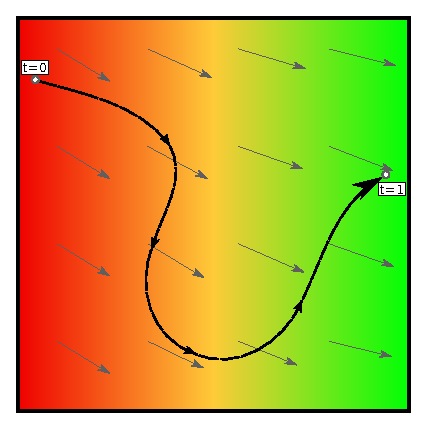
\includegraphics[width=8cm]{images/swimmer_in_water}
\caption{Die Bahn eines Bootes im Wasser. Die Temperatur des Fluids ist hier durch Farben kodiert. Rot bedeutet warmes Wasser, grün bedeutet kaltes Wasser. Nicht dargestellt ist die Veränderung der Wassertemperatur über die Zeit.}
\end{figure}

Sowohl die Euler'sche- als auch die Lagrang'sche Betrachtungsweise spiegeln sich
in den Navier-Stokes-Gleichungen wider. Obwohl es nicht sofort
erkennbar ist, bilden die Gleichungen eine Entsprechung der Gleichung
$\vec{F} = m \cdot \vec{a}$ mit dem Unterschied, dass keine Kraft auf
einen einzelnen Körper berechnet wird, sondern auf einen ganzen
Raumabschnitt (ein \PimiddyQuotes{Kontinuum}).

Was die beiden Betrachtungsweisen verbindet, ist die
\PimiddyBegriff{substantielle Ableitung}. Zur Herleitung dieser
Ableitungsform betrachten wir zunächst eine beliebige Größe
$q(\vec{x},t)$. Dies kann eine skalare Größe wie z.\,B.\ die Temperatur
eines Gewässers sein oder eine Vektorgröße wie die Farbe des Wassers
an einem Punkt. Da $q$ in jedem Punkt definiert ist, stellt die
Funktion eine Euler'sche Größe dar.

Zudem betrachten wir ein Partikel mit einer Bewegungsbahn durch das
Fluid (z.\,B.\  ein Ruderboot im Wasser). Seine Position zum Zeitpunkt
$t$ sei gegeben durch $\vec{p}(t)$. Dies entspricht einer
Lagrange'schen Größe.

Setzen wir beide Größen zusammen, erhalten wir beispielsweise die
Temperatur des Wassers auf der Bahn, die das Boot im Wasser verfolgt:

\begin{equation}
\PimiddyFormelText{Temperatur}(t) = q(\vec{p}(t),t)
\end{equation}

Wollen wir wissen, wie sich die Umgebungstemperatur des Bootes im Lauf
der Zeit verändert, bilden wir die (totale) Ableitung dieser
zusammengesetzten Größe:

\begin{equation}
\frac{
	\partial \PimiddyFormelText{Temperatur}(t)
}
{
	\partial t
}
=
\frac{
	\partial q
}
{
	\partial t
}
+
\PimiddyGrad q \cdot
\frac{
	\partial \vec{p}}
{
	\partial t
}
\end{equation}

Die Summe auf der rechten Seite besteht aus zwei Teilen. Der erste Term,
$\frac{\partial q}{\partial t}$, gibt an, wie sich das Fluid unabhängig von
der betrachteten Position verändert. Bezogen auf das Boot gibt dieser
Term an, wie sich die Temperatur des Gewässers über den Tag verteilt
verändert, beispielsweise durch den Einfluss der Sonnenstrahlen. Der
zweite Term ergänzt die globale Ableitung durch die lokale
Temperaturänderung, die durch die Bahn des Bootes verursacht
wird.

Statt eines beliebigen Pfades durch das Fluid nimmt man zur Definition der
substantiellen Ableitung nun das Geschwindigkeitsfeld des Fluids zur Hilfe:

\begin{equation}
\frac{
	Dq}
{
	Dt
} :=
\frac{
	\partial q
}
{
	\partial t
}
+
\PimiddyGrad q \cdot
\vec{u}
\end{equation}

Man geht also von einem Partikel aus, was sich im Fluid \PimiddyQuotes{treiben}
lässt, und misst die Veränderung der Größe $q$ auf seiner Bahn. Analog ist die
substantielle Ableitung für Vektorgrößen definiert:

\begin{equation}
\frac{
	D\vec{q}}
{
	Dt
} :=
\frac{
	\partial q
}
{
	\partial t
}
+
\PimiddyDiv q \cdot
\vec{u}
\end{equation}

Die Impulsgleichung lässt sich mit Hilfe der substantiellen Ableitung so schreiben:

\begin{equation}
\rho \frac{D\vec{u}}{Dt} = - \PimiddyGrad p + \PimiddyLaplace \vec{u} + \vec{f}
\end{equation}

Dies entspricht der klassischen Newton'schen Kraftformel, wobei die
Masse $m$ durch die Dichte $\rho$ ersetzt wird. Auf der rechten Seite
der Gleichung stehen die Kräfte, die das Fluid beeinflussen. Diese
Kräfte sollen im Einzelnen näher beschrieben werden.

\subsubsection{Die Kräfte in den Navier-Stokes-Gleichungen}

Die Kraft, die überall im Fluid in gleicher Weise wirkt, ist die Schwerkraft:

\begin{equation}
F_g =
\left(
\begin{array}{c}
0 \\
-g \\
0
\end{array}
\right)
\end{equation}

mit $g \cong 9.81 \frac{m}{s^2}$.

Durch den Druck $p$ des Fluids wird eine weitere Kraft $F_p$ ausgeübt.
Allerdings erzeugt die Anwesenheit von Druck (also $p \neq 0$) allein
keine Kraft. Ist der Druck beispielsweise im gesamten Fluid konstant,
ist die ausgeübte Kraft gleich 0. Stattdessen wirkt $F_p$
\PimiddyQuotes{ausgleichend}. Sie zeigt von Bereichen hohen Drucks hin
zu Bereichen niedrigeren Drucks. Mathematisch gesehen ist $F_p$ also
proportional zum negativen Gradient des Drucks.

\begin{equation}
\label{eq:navier_stokes_f_p}
F_p = -\PimiddyGrad p
\end{equation}

 In \autoref{fig:navier_stokes_particle_system_wall_collision}) ist
dies intuitiv anhand eines Partikelsystems erläutert. Treffen die
Partikel auf eine Wand, entsteht Druck, der tangential zur Wand wirkt
und die Partikel in diese Richtung beschleunigt. In den späteren
Berechnungen spielt der Druck insbesondere eine Rolle, um das Fluid in
seinem unkomprimierbaren Zustand zu halten und um das Hineinfließen in
Hindernisse zu verhindern.

\begin{figure}[ht]
\centering
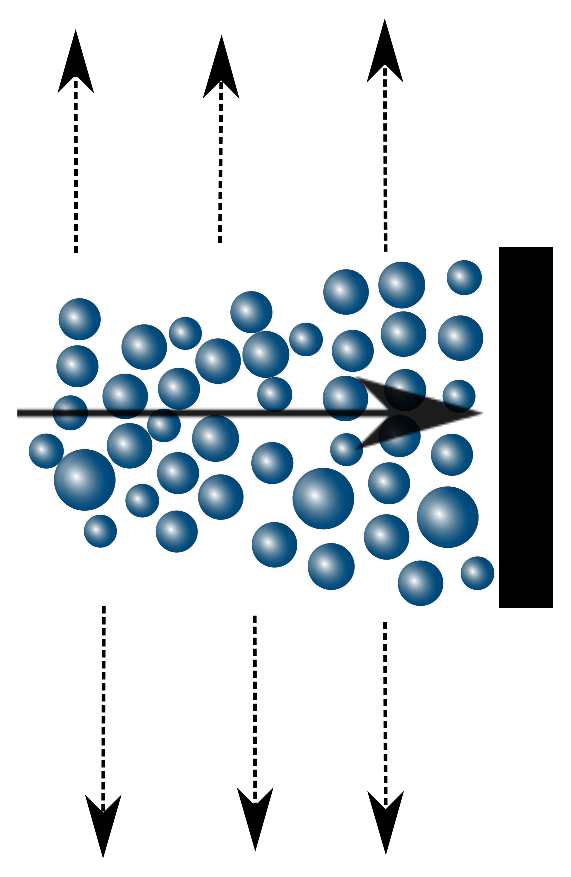
\includegraphics[width=6cm]{images/particle_system_wall_collision}
\caption{Partikelsystem, das auf ein Hindernis prallt. Der durchgezogene Pfeil deutet die Fließrichtung an, die gestrichelten Pfeile den negativen Gradienten des Drucks. Die Partikel erfahren also eine Kraft nach außen.}
\label{fig:navier_stokes_particle_system_wall_collision}
\end{figure}

Die Viskosität des Fluids hat ebenfalls Einfluss auf das Fluid. Bei einem
viskosen Fluid wird jeder Deformation ein Widerstand entgegengesetzt. Eine
Flüssigkeit wie Honig, die um ein Hindernis herumfließt, bildet hinter dem
Hindernis keine Verwirbelungen; die hohe Viskosität wirkt dem entgegen. Luft
hingegen hat eine niedrige Viskosität, bildet also besonders viele Wirbel.

Die Kraft, die durch die Viskosität ausgeübt wird, hat den Effekt,
Geschwindigkeitsunterschiede innerhalb des Fluids auszugleichen. Sie ist
daher proportional zum Laplace der Geschwindigkeit:

\begin{equation}
\label{eq:navier_stokes_f_v}
F_v = \mu \cdot \PimiddyLaplace \vec{u}
\end{equation}

Die Konstante $\mu$ stellt die \PimiddyBegriff{dynamische Viskosität}
des Fluids dar.

\subsection{Die Unkomprimierbarkeitsbedingung}
\label{sec:mathematics_incompressibility_condition_section}

\begin{figure}[ht]
\centering
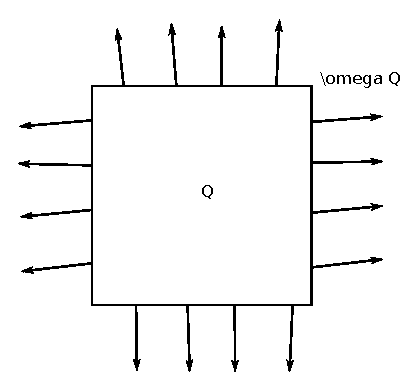
\includegraphics[width=10cm]{images/incompressibility_condition_example}
\caption{Fluss durch ein Rechteck. Der große Pfeil deutet die Fließrichtung des Fluids an. Die Pfeile an den Rändern des Rechtecks zeigen in die dortige Fließgeschwindigkeit, über deren Normalenkomponente in \autoref{eq:navier_stokes_incompressibility_initial_integral} integriert wird.}
\label{fig:navier_stokes_incompressibility_condition_example}
\end{figure}

Um die Unkomprimierbarkeitsbedingung zu motivieren, sei ein beliebiges Volumen
$\Omega \subset \PimiddyReell^3$ gegeben, \PimiddyzB ein Würfel im Raum. Seine
Oberfläche sei $\partial \Omega$.

Die Änderung des Würfelvolumens über die Zeit kann berechnet werden,
indem man über die Normalenkomponente entlang seiner Oberfläche
integriert \cite{Chorin1980}. Bildlich gesprochen summiert man auf
diese Weise eingehende und ausgehende Strömungen an den
Würfelseitenflächen (\Pimiddyvgl
\autoref{fig:navier_stokes_incompressibility_condition_example}):
\begin{equation}
\label{eq:navier_stokes_incompressibility_initial_integral}
\frac{
	\partial \PimiddyFormelText{Volumen}(\Omega)
}
{
	\partial t
}
=
\iint_{\partial \Omega} \vec{u} \cdot \vec{n}
\end{equation}
Damit die Flüssigkeit unkomprimierbar ist -- sich das Volumen also
nicht ändert -- sollte dieses Integral verschwinden:
\begin{equation}
\iint_{\partial \Omega} \vec{u} \cdot \vec{n} = 0
\end{equation}
Mit Hilfe des Divergenzsatzes können wir dieses Integral in ein Volumenintegral
umformen:
\begin{equation}
\iiint_\Omega \PimiddyDiv \vec{u} = 0
\end{equation}
Da $\Omega$ beliebig gewählt war, folgt die
Unkomprimierbarkeitsbedingung $\PimiddyDiv \vec{u} = 0$.

\section{Methode nach Stam}

\subsection{Motivation}

Die Methode zur approximativen Lösung der Navier-Stokes-Gleichungen, die im
Folgenden erklärt wird, wurde von \PimiddyName{Jos Stam} im Jahr 1999 entwickelt
und in dem Paper "`Stable Fluids"' vorgestellt \cite{Stam1999}. Das Verfahren
wurde speziell für die Computergrafik entwickelt, wobei auf einige
Besonderheiten eingegangen wurde:

\begin{enumerate}
\item
	Im Gegensatz zu wissenschaftlichen Simulationen ist man in der
	Computergrafik an einer Lösung interessiert, die in möglichst kurzen
	Abständen Ergebnisse produziert. Zum Beispiel möchte man die
	Strömungssimulation jedes Frame um einen Zeitschritt weiterbewegen. Um
	eine flüssige Simulation zu erhalten, ist die Laufzeit des
	Lösungsalgorithmus also auf 16 Millisekunden (für 60 Bilder pro Sekunde)
	bzw. 33 Millisekunden (für 30 Bilder pro Sekunde) beschränkt. Die
	Navier-Stokes-Gleichungen bilden als System von nichtlinearen
	Differentialgleichungen hier eine besondere Herausforderung.
\item
	Man ist außerdem nicht unbedingt an einer exakten Lösung interessiert.
	Will man z.\,B. Wasser oder Rauch simulieren reicht es, ein physikalisch
	annähernd korrektes Verhalten zu erzielen.
\item
	Bisherige Verfahren (wie z.\,B. die finiten Differenzen in
	\cite{Foster1997}) waren numerisch \emph{instabil} für große
	Zeitschritte. Dynamische Anwendungen wie Spiele oder Animationssoftware
	können allerdings keine minimiale Framerate garantieren, da sie mit
	verschiedenen Umgebungen und Hardwarekonfigurationen ausgeführt werden
	können.

	Als Ausweg muss man einen großen Zeitschritt (ein langes Frame) entweder
	ignorieren -- was die Simulation unrealistisch macht -- oder ihn in
	kleinere Zeitschritte unterteilen. Die Laufzeit des Verfahrens ist aber
	im Allgemeinen nicht von der Größe des Zeitschritts abhängig. Dies führt
	dazu, dass das nächste Frame erneut viel Rechenzeit benötigt und wieder
	entsprechend lang wird.

	Dieser Effekt ist nicht mehr aufzuhalten und die Simulation
	\PimiddyQuotes{explodiert}.
\item
	Bisherige Verfahren waren auf Hilfe des Designers angewiesen, um Teile
	der Simulation möglichst realistisch zu modellieren. Bestimmte natürlich
	vorkommende Turbulenzen mussten explizit in die Simulation eingegeben
	werden. Idealerweise sollte die Simulation allerdings von selber
	fortgeführt werden, der Designer sollte nur Rahmenbedingungen wie
	Hindernisse und globale Eigenschaften des Fluids (wie Dichte und
	Viskosität) vorgeben.
\end{enumerate}

\begin{figure}[ht]
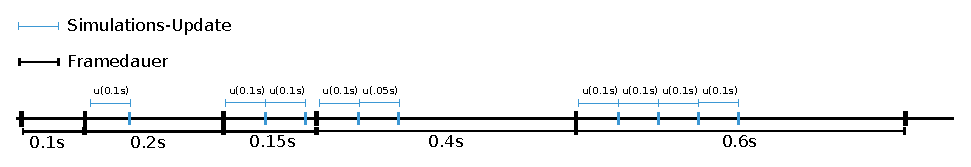
\includegraphics[width=12cm]{images/simulation_blowup}
\caption{Instabilität in Simulationen: Hier wird angenommen, die maximal zu simulierende Simulationsdauer sei $0.1s$. Längere Frames werden in mehreren Ticks berechnet, die aber konstant lange Laufzeit haben. Dies führt zu dauerhaft langen Frames, der Effekt potenziert sich.}
\end{figure}

Das Verfahren ist also auf Geschwindigkeit ausgelegt, basiert aber
nichtsdestotrotz auf den Navier-Stokes-Gleichungen und erzielt akkurate
Simulationsergebnisse. Anfängliche Schwachstellen des Verfahrens wie die zu
starke Dämpfung von Wirbeln wurden in weiteren Arbeiten ausgebessert
\cite{Foster}. Diese Verbesserungen sind teilweise auch in die Arbeit
eingeflossen.

Wegen der numerischen Stabilität und sehr guten Parallelisierbarkeit wird Stams
Verfahren bereits in einigen Spielen eingesetzt (siehe \cite{Crane2007},
\cite{Peschel2009}). Hier beschrieben wird eine leicht abgewandelte
Fassung, bei der andere Randbedingungen verwendet werden.

\subsection{Überblick über das Verfahren}

Die Fluidsimulation findet auf einem diskreten, endlichen Gitter, also einer
Teilmenge von $\PimiddyGanz^n$ statt. Gegeben sei das Geschwindigkeitsfeld zum
Zeitpunkt $t$: $\vec{u}_{i,j,k}^t$. Als Anfangsbedingung könnten zum Zeitpunkt $0$
z.\,B. alle Zellen auf eine vorgegebene \PimiddyQuotes{Windrichtung} gesetzt sein.
Gegeben sei außerdem ein Zeitdelta $\Delta t$ (nicht zu verwechseln mit dem
Laplaceoperator). Ziel ist es, unter Zuhilfenahme der
Navier-Stokes-Gleichungen ein neues Geschwindigkeitsfeld $\vec{u}_{i,j,k}^{t+\Delta
t}$ zu berechnen.

Außerdem berechnen wir einmalig ein \emph{Hindernisfeld} $b_{i,j,k}$. Ist $b_{i,j,k}
= 1$, dann ist diese Zelle mit einem Hindernis ausgefüllt. Ist $b_{i,j,k} = 0$,
ist die Zelle frei. Im Implementierungsteil wird erklärt, wie dieses
Hindernisfeld gefüllt wird.

Die rechte Seite der Impulsgleichung \eqref{eq:navier_stokes_momentum_equation} besteht
aus mehreren Summanden:

\begin{equation}
\vec{u} \PimiddyDiv \vec{u} -
\nu \PimiddyLaplace \vec{u} +
\vec{g} -
\frac{
	1
}
{
	\rho
}
\PimiddyGrad p
\end{equation}

In Stams Verfahren wird jeder dieser Summanden als eine Operation betrachtet,
die ein Geschwindigkeitsfeld sowie eventuell weitere Eingabegrößen wie $\Delta
t$ erhält, und die ein neues Geschwindigkeitsfeld zurückgibt. Das so berechnete
neue Feld wird zur Eingabe der darauffolgenden Operation. So wird die Lösung der
Impulsgleichung in kleinere Teile zerlegt, die für sich behandelt werden können:

\begin{itemize}
\item
	Der Term
	\begin{equation}
	\vec{u} \PimiddyDiv \vec{u}
	\end{equation}
	stellt die \PimiddyBegriff{Advektion} dar. Das Vektorfeld wird entlang
	seiner eigenen Strömungsrichtung weiterbewegt. Er sei im Folgenden mit
	\PimiddyInlineCode{advection}$(\vec{u},\Delta t)$ bezeichnet.
\item
	Der Term
	\begin{equation}
	\nu \PimiddyLaplace \vec{u}
	\end{equation}
	stellt die viskose \PimiddyBegriff{Diffusion} dar. Selbst wenn keine
	Kräfte auf das Fluid wirken, bewegt es sich durch Diffusionsprozesse
	weiter, so wie Farbe auf einem Blatt Papier verläuft.

	Dieser Term kann in Stams Verfahren ignoriert werden. Diffusion entsteht
	ohnehin \PimiddyQuotes{zufällig} durch Genauigkeitsfehler während der
	Advektion (siehe unten). So kann Performance eingespart werden, denn die
	Lösung dieses Terms ist sehr aufwändig.
\item
	Der Term $\vec{g}$ umfasst schlicht das Aufsummieren aller äußeren
	Kräfte, die auf das Fluid wirken. Hierzu gehört sowohl die Schwerkraft
	als auch der von außen eingeführte Wind. Die Operation bekommt als
	Eingabe das Geschwindigkeitsfeld sowie das Zeitdelta (bei größerem
	Zeitunterschied zum letzten Simulationsschritt sollen die Kräfte
	stärker wirken). Sei sei im folgenden mit
	\PimiddyInlineCode{externalForces}$(\vec{u},\Delta t)$ bezeichnet.
\item
	Der \emph{Druck} des Fluids wird in dem Term
	\begin{equation}
	-\frac{1}{\rho} \PimiddyGrad p
	\end{equation}
	zusammengefasst. Er dient am Ende unter anderem dazu, die
	Randbedingungen und die Un"-komp"-ri"-mier"-bar"-keit zu erzwingen. Die Berechnung
	des Drucks sei mit \PimiddyInlineCode{calculatePressure}$(\vec{u})$
	bezeichnet.
\item
	Wie bei Differentialgleichungen üblich, müssen wir noch die
	\emph{Rand- und Anfangsbedingungen} behandeln. Dadurch wird
	einerseits sichergestellt, dass der das Fluid nicht in Hindernisse
	eindringt, andererseits an den Rändern der Simulation frei hinausfließen
	kann. Diese Operation wird im Folgenden als
	\PimiddyInlineCode{boundaries}$(\vec{u})$ bezeichnet und wird vor der
	Berechnung des Drucks eingefügt.
\end{itemize}

\begin{algorithm}
\caption{Der Lösungsalgorithmus in Pseudocode}
\label{alg:stam_first_algorithm}
\begin{algorithmic}
\Function{simulate}{$\vec{u}$,$\Delta t$}
	\State $\vec{u}'$ = advection($\vec{u}$,$\Delta t$)
	\State $\vec{u}''$ = externalForces($\vec{u}'$,$\Delta t$)
	\State $\vec{u}'''$ = boundaries($\vec{u}''$)
	\State $p$ = calculatePressure($\vec{u}$)
	\State \Return $\vec{u}''' - \PimiddyGrad p$
\EndFunction
\end{algorithmic}
\end{algorithm}

\begin{figure}[ht]
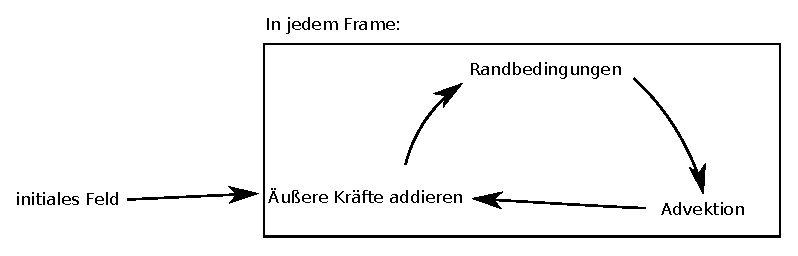
\includegraphics[width=10cm]{images/stam_loop}
\caption{Die Simulationsschleife ohne Projektion.}
\end{figure}

Für jeden Term wird im Folgenden ein Lösungsalgorithmus vorgestellt, insgesamt
erhält man den Pseudocode in \autoref{alg:stam_first_algorithm}.

\subsection{Advektion}

Wie bereits in der Erklärung der Navier-Stokes-Gleichungen angedeutet, wird bei
der Advektion das Geschwindigkeitsfeld entlang \PimiddyQuotes{sich selber}
weiterbewegt. Auf diese Weise kann sich Wind, der von einer Seite der
Simulation eingeführt wird, über den gesamten Simulationsbereich ausbreiten.
Manchmal spricht man daher auch von \emph{Selbstadvektion}. In älterer Literatur
ist auch von \emph{Konvektion} die Rede.

Im Folgenden gehen wir etwas allgemeiner davon aus, dass eine \emph{beliebige} Größe
$q_{i,j,k}^t$ entlang des Vektorfelds $\vec{u}$ bewegt werden soll. Die Methode
\PimiddyInlineCode{advection} kann also auch verwendet werden, um
Temperaturwerte oder die Dichte des Rauchs an einer Stelle entlang des
Vektorfeldes weiterzubewegen. Als Ausgabe erhalten wir ein neues Feld
$q_{i,j,k}^{t+\Delta t}$.

Um die Advektion durchzuführen gibt es mehrere Ansätze. Der gängigste arbeitet
mit der Methode der finiten Differenzen und wurde unter anderem in
\cite{Foster} benutzt. Finite Differenzen führen aber zu einem numerisch
instabilen Algorithmus. Im Gegensatz dazu soll hier zunächst ein intuitiver
Ansatz erläutert werden, der auch numerisch instabil ist und somit nicht ohne
große Einschränkungen verwendbar ist. Dieser Ansatz wird danach leicht
modifiziert, um Stabilität zu erreichen.

\begin{figure}[ht]
\centering
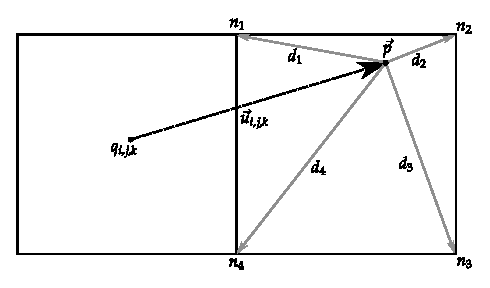
\includegraphics[width=6cm]{images/advection_bad}
\caption{Das numerisch instabile Advektionsverfahren}
\label{fig:stam_numerically_unstable_advection}
\end{figure}

Das neue Feld $q_{i,j,k}^{t+\Delta t}$ sei anfangs überall 0 (bzw\,. $(0,0,0)$,
falls es ein Vektorfeld ist). Man stelle sich an jedem Gitterpunkt
$(i,j,k)$ ein Partikel mit \PimiddyQuotes{Ladung} $q_{i,j,k}$ vor, was im Fluid
treibt. Durch die Bewegung des Fluids würde dieses Partikel um $\Delta t \cdot
\vec{u}_{i,j,k}$ verschoben und läge im nächsten Zeitschritt bei
$\vec{p}=(i,j,k)+\Delta t \cdot \vec{u}_{i,j,k}$. Somit läge es im Allgemeinen
nicht mehr \emph{exakt} auf einem Gitterpunkt, sondern zwischen 8 Nachbarpunkten
$n_i \in \PimiddyGanz^3, i \in \{1,\ldots,8\}$ (siehe
\autoref{fig:stam_numerically_unstable_advection}). Man bestimmt jetzt die
Distanz von $\vec{p}$ zu jedem der Nachbarpunkte:

\begin{equation}
d_i = \PimiddyNorm{2}{\vec{p} - n_i}, i \in \{1,\ldots,8\}
\end{equation}

Diese $d_i$ dienen als Gewichtung, um die \PimiddyQuotes{Ladung} $q_{i,j,k}$
anteilig auf die Nachbarknoten aufzuteilen:

\begin{equation}
q_{n_i}' \leftarrow q_{n_i}' + d_i \cdot q_{i,j,k}
\end{equation}

Dieses Verfahren ist intuitiv und einfach zu implementieren. Aber es ist
numerisch nicht stabil und führt zu Oszillationen (für eine genaue Betrachtung
sei auf die Literatur verwiesen).

Stam wählte einen anderen Ansatz, die sogenannte \emph{Methode der
Charakteristika}. Die Idee ist ähnlich zu der gerade vorgestellten, funktioniert
aber in die \PimiddyQuotes{umgekehrte Richtung}.

\begin{figure}[ht]
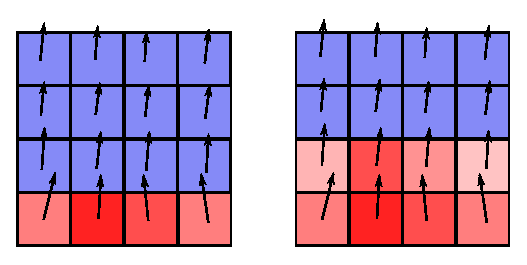
\includegraphics[width=6cm]{images/advection_bad_example}
\caption{Das numerisch instabile Advektionsverfahren für ein Temperaturfeld}
\end{figure}

Man betrachtet wieder jeden Gitterpunkt $(i,j,k)$ einzeln, stellt sich diesmal
allerdings vor, man sei auf der Zeitachse im Punkt $t+\Delta t$, also bereits im
nächsten Zeitschritt. Das (gedachte) Partikel an Position $(i,j,k)$ habe die
Geschwindigkeit $\vec{u}_{i,j,k}^t$.

Rechnet man auf der Zeitachse um $\Delta t$ zurück, erhält man die
\PimiddyQuotes{vorherige} Position des Partikels, nämlich $(i,j,k) - \Delta t
\cdot \vec{u}_{i,j,k}^t$ \PimiddyFootnote{Hier wird nur ein Schritt der
Partikelflugbahn zurückverfolgt. Es besteht die Möglichkeit, mehrere
Schritte zurückzuverfolgen, die ist aber aufwändig zu implementieren.}. Es
ergibt sich allerdings dasselbe Problem wie bei dem vorher beschriebenen Ansatz:
Diese Position liegt nicht genau auf dem Gitter, sondern dazwischen (siehe
\autoref{fig:stam_good_advection}).

Als Lösung \emph{interpolieren} wir zwischen den 8 Nachbarwerten des
verschobenen Partikels und schreiben den entstehenden Wert in die Zelle
$u_{i,j,k}^{t+\Delta t}$. Dies ist eine Operation, auf die Grafikkarten stark
optimiert sind, und bei denen traditionell Texturen hohe Performance erreichen
können.

Allerdings liegt hier auch eine Fehlerquelle des Verfahrens. Interpolation ist
eine glättende Operation, sie liefert nur eine \emph{Approximation} des Wertes,
der zwischen den Gitterzellen angenommen würde. Ähnlich wie bei der
Herleitung der diskreten Ableitung in \autoref{sec:mathematics_discretization}
muss man in der Implementierung einen Kompromiss eingehen und ein
Interpolationsverfahren wählen, was Genauigkeit und Rechenleistung verbindet.

Auch für große Zeitschritte liefert das Verfahren ein Vektorfeld als Ausgabe,
was in seinem Wertebereich beschränkt ist, denn die Interpolation liefert kein
Wert zurück, der betragsmäßig größer ist als die Ausgangswerte. Das Verfahren
ist deshalb stabil. Allerdings sollte $\Delta t$ nicht zu groß gewählt werden.
\cite{Foster} gibt hier als Richtlinie etwa $5\times$ die Gittergröße an.

\begin{figure}[ht]
\centering
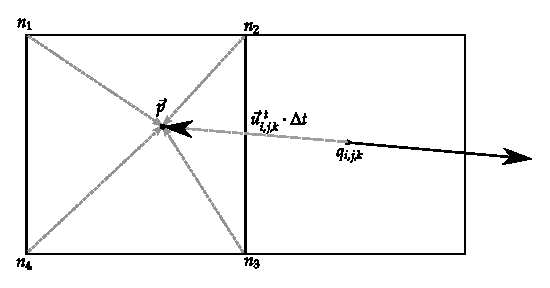
\includegraphics[width=6cm]{images/advection_good}
\caption{Stams stabiles Advektionsverfahren}
\label{fig:stam_good_advection}
\end{figure}

Natürlich kann es passieren, dass wir über den Rand des Simulationsbereiches
\PimiddyQuotes{hinauslaufen}. Es gibt mehrere Möglichkeiten, dies zu behandeln.
Beispielsweise könnte man auf die gegenüberliegenden Seite des
Simulationsbereiches umbrechen (periodische Randbedingung), was in Stams Arbeit
getan wurde. Alternativ kann man die Gerade betrachten, die durch den
Mittelpunkt der aktuellen Zelle geht, und diese Gerade mit den Rändern der
Simulation schneiden. Man wählt dann den Schnittpunkt auf dem Rand als Basis für
die Interpolation (siehe \autoref{fig:stam_clamping_borders}). Dies wurde in der
Arbeit implementiert.

\begin{figure}[ht]
\centering
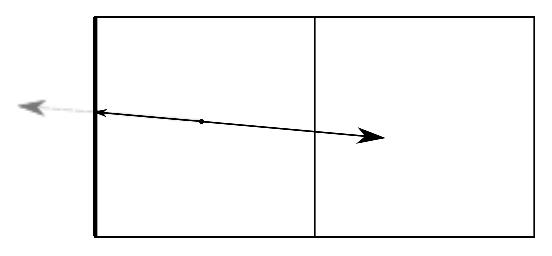
\includegraphics[width=6cm]{images/advection_clamping_borders}
\caption{Abschneiden der Geschwindigkeit an den Rändern}
\label{fig:stam_clamping_borders}
\end{figure}

Weiterhin kann der zurückberechnete Vektor $(i,j,k) - \Delta t u_{i,j,k}^t$ in
einem Hindernis landen. Man kann in diesem Fall einen Geschwindigkeitswert
von $(0,0,0)$ annehmen, was einem stationären Hindernis wie einem Gebäude
entspricht. Es ist aber auch möglich, ein weiteres Vektorfeld
$\vec{u}_{\PimiddyFormelText{boundary}}$ zu verwalten, wo für jede Gitterzelle die
\emph{Geschwindigkeit} des dort vorhandenen Hindernisses notiert ist. Dies wurde
in \cite{Crane2007} umgesetzt. Für die Simulation in dieser Arbeit wurde von
unbeweglichen Hindernissen ausgegangen.

\PimiddyTodo{Hier kurz erklären, dass das auch Semilagrangeadvektion genannt wird.}

\subsection{Äußere Kräfte}

\subsubsection{Gravitation}

Zu den äußeren Kräften gehört zu allererst die \emph{Gravitation}. Diese lässt
sich sehr einfach ausdrücken:

\begin{equation}
F_g = \Delta t (0,-9.81,0)
\end{equation}

\subsubsection{Auftrieb}

\PimiddyTodo{Auftrieb allgemein und konkret mit Buissnesq erklären}

\subsubsection{Wirbelstärkenerhaltung}

Der Advektionsschritt enthält eine lineare Interpolation, um die
Geschwindigkeitswerte in der Nachbarschaft des zurückverfolgten Partikels zu
finden. Diese simple Interpolationsmethode führt allerdings dazu, dass
Genauigkeit bei der Simulation verloren geht. Dadurch werden viele interessante
Phänomene in Fluiden, wie die starke Wirbelbildung bei Rauch, gedämpft und
treten nicht mehr so stark in Erscheinung.

Um dies auszugleichen, gibt es mehrere Ansätze. MacCormack hat ein
Advektionsverfahren entwickelt, was nicht mehr unbedingt stabil ist, aber eine
bessere Fehlerabschätzung liefert \cite{Selle2008}\cite{Crane2007}. Dadurch
entstehen mehr Wirbelphänomene, allerdings bietet diese Methode keinen Einfluss
darauf, wie stark die Wirbel auftreten sollen.

Statt des MacCormack-Verfahrens wurde hier eine Technik namens
\PimiddyBegriff{Wirbelstärkenerhaltung} (\PimiddyEnglisch{vorticity
confinement}) umgesetzt. Sie ist einfach zu implementieren, schnell und
erlaubt, die Stärke zu variieren. Entwickelt wurde sie, um die komplexen
Turbulenzen in der Umgebung von Helikoptern zu modellieren\cite{Steinhoff1994}.

Die Idee ist, Wirbel zu identifizieren und an den \PimiddyQuotes{richtigen}
Stellen zu verstärken. Dazu wird zuerst die Rotation des Geschwindigkeitsfeldes,
$\vec{R} = \PimiddyRot \vec{u}_{i,j,k}$, bestimmt. Der Betrag der Rotation,
$|\vec{R}|$, gibt an, wie stark die Rotation in einem Punkt ist. Der
\emph{Gradient} des Betrags, $\PimiddyGrad |\vec{R}|$, zeigt also
von Bereichen niedriger Wirbelstärke zu bereichen hoher Wirbelstärke.

Um die Wirbel zu verstärken, bildet man eine Kraft, die senkrecht zum
(normalisierten) Gradienten und zur Rotation ist:

\begin{equation}
\label{eq:stam_vorticity_confinement}
\vec{F}_{\PimiddyFormelText{vorticity}}
=
\varepsilon \cdot
\left(
	\frac
	{
		\PimiddyGrad \vec{R}
	}
	{
		|\PimiddyGrad \vec{R}|
	}
	\times
	\vec{R}
\right)
\end{equation}

Die Konstante $\varepsilon$ in \autoref{eq:stam_vorticity_confinement} gibt die
Stärke der Kraft an.

\subsection{Projektion}

\subsubsection{Einleitung}

Die vorgestellten Al"-go"-rith"-men be"-rück"-sich"-ti"-gen die
Un"-komp"-ri"-mier"-bar"-keit des Flu"-ids nicht. Nach der Advektion und der
Addition der äußeren Kräfte kann die zweite Bedingung
\ref{eq:navier_stokes_incompressibility_condition} in den
Navier-Stokes-Gleichungen also verletzt sein, und die Simulation somit nicht
mehr physikalisch korrekt. Außerdem sind die Randbedingungen eventuell verletzt
worden. Beispielsweise wurde bei der Advektion nicht beachtet, dass das Fluid um
Hindernisse herumströmen sollte. Für beide Fälle kommt der Druck $p$ als
Korrekturterm ins Spiel.

Gegeben sei ein beliebiges Vektorfeld $\vec{u}$. Gesucht ist eine Funktion
$\PimiddyProjection$, die dieses Vektorfeld auf ein quellenfreies Vektorfeld
abbildet, also eins mit $\PimiddyDiv \vec{u} = 0$. Hierzu bedient man sich eines
Ergebnisses aus der Vektoranalysis:

\begin{PimiddySatz}[Helmholtz-Zerlegung]
Sei $\vec{u}$ ein zweimal stetig differenzierbares Vektorfeld auf einem
beschränkten Definitionsbereich, dann lässt $\vec{u}$ sich zerlegen in
ein \emph{quellenfreies} Vektorfeld $\vec{w}$ und den \emph{Gradienten}
eines Skalarfeldes $p$:

\begin{equation}
\label{eq:stam_helmholtz_equation}
\vec{u} = \vec{w} + \PimiddyGrad p
\end{equation}
\end{PimiddySatz}

\autoref{eq:stam_helmholtz_equation} soll nach $\vec{w}$ aufgelöst werden, sodass
dieses Feld für die nächste Iteration des Lösungsalgorithmus verwendet werden
kann. Das Feld $p$ ist aber ebenfalls eine Unbekannte. Um die Gleichung
aufzulösen, wendet man die Divergenz auf beide Seiten der Gleichung an und nutzt
aus, dass der Operator \emph{linear} ist. Es gilt also

\begin{equation}
\PimiddyDiv (\vec{u} + \vec{v}) = \PimiddyDiv \vec{u} + \PimiddyDiv \vec{v}
\end{equation}

Als Ergebnis erhalten wir:

\begin{equation}
\label{eq:stam_poisson_equation}
\PimiddyDiv \vec{u} = \PimiddyLaplace p
\end{equation}

Hier wurde ausgenutzt, dass $\PimiddyDiv \vec{w} = 0$ gilt. Dies ist eine
sogenannte \PimiddyBegriff{Poissongleichung}. Ihre Lösung ist ein
Standardproblem in der Physik, und im Folgenden wird ein Verfahren vorgestellt,
was \autoref{eq:stam_poisson_equation} nach $p$ auflösen kann. Mit $p$ kann man
dann durch Umstellen und Bildung des Gradienten $\vec{w}$ bestimmen:

\begin{equation}
\vec{w} = \vec{u} - \PimiddyGrad p
\end{equation}

Darauf aufbauend kann man jetzt den Operator $\PimiddyProjection$ definieren

\begin{equation}
\PimiddyProjection \colon \PimiddyReell^n \to \PimiddyReell^n
\end{equation}

als die Funktion, die ein Vektorfeld auf den quellenfreien Anteil der
Helmholtz-Zerlegung abbildet (ein Vektorfeld also quellenfrei
\PimiddyQuotes{macht}). Diese Funktion wird in der Literatur auch oft
\PimiddyBegriff{Projektion} genannt. Führt man $\PimiddyProjection$ am Ende des
Algorithmus' aus, erhält man ein unkomprimierbares Vektorfeld.

\begin{figure}[ht]
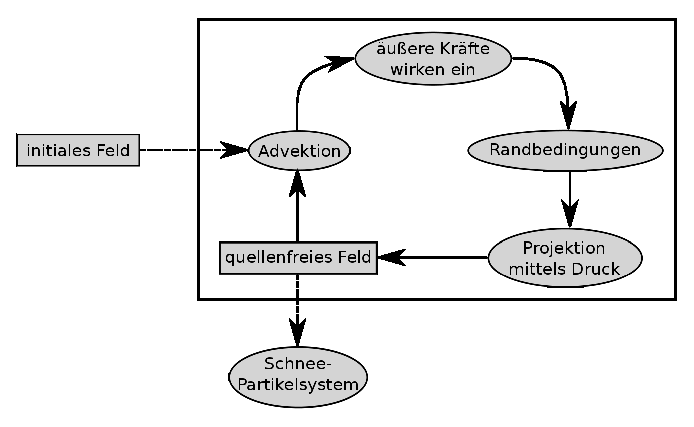
\includegraphics[width=10cm]{images/stam_loop_with_projection}
\caption{Die Simulationsschleife mit Projektion.}
\end{figure}

\subsubsection{Lösung des Poissonproblems}

Um das Vektorfeld quellenfrei zu machen, muss folgende
\PimiddyBegriff{Poissongleichung} nach $p$ gelöst werden:

\begin{equation}
\PimiddyLaplace{p} = x
\end{equation}

wobei $x$ ein Skalarfeld ist. Es existieren zahlreiche Lösungsverfahren für solch
eine Gleichung. Bei der Auswahl des Verfahrens muss beachtet werden, welches
Verfahren sich gut auf der Grafikkarte umsetzen lässt und möglichst schnell eine
ausreichend gute Lösung liefert.

Es haben sich mehrere sogenannte \PimiddyBegriff{Iterationsverfahren} als
günstig herausgestellt. Verfahren dieser Art beginnen mit einer initialen Lösung
(beispielsweise schlicht $p=0$) und nähern sich dann in jedem Iterationsschritt
weiter der eigentlichen Lösung an.

Betrachtet man große Felder, bieten sich \PimiddyBegriff{Mehrgitterverfahren}
an. Diese wurde bereits erfolgreich auf GPUs angewendet (siehe \cite{Bolz2002},
\cite{Matthias2006}). Sie sind allerdings untrivial zu implementieren, da intern
ein zweites Iterationsverfahren benötigt wird (der sogenannte
Restriktionsoperator), sowie Methoden zum hoch- und runterskalieren von
3D-Feldern.

Simplere Iterationsverfahren sind SOR (\cite{Saltvik2006}),
Gauss-Seidel-Re"-la"-xa"-ti"-on (\cite{Stam2003}) und das
Jacobiverfahren (\cite{Crane2007}, \cite{Harris2008},
\cite{Peschel2009}). Letzteres ist besonders einfach zu
implementieren und gleichzeitig hervorragend für die GPU geeignet.

\subsubsection{Das Jacobiverfahren}

Um das Jacobi-Verfahren zu veranschaulichen, soll es zunächst im
Eindimensionalen erläutert werden. Wir betrachten also kein diskretes 3D-Gitter,
sondern eine endliche Teilmenge der ganzen Zahlen (die Gitterbreite $\Delta x$
ist also $1$). Der Laplaceoperator entspricht in diesem Fall der zweiten
Ableitung von $p$.

Für die exakte Lösung $p$ des Poissonproblems muss an jeder Stelle $i$ gelten:

\begin{equation}
\label{eq:stam_jacobi_onedimensional}
\frac{
	p_{i+1} -
	2 \cdot p_{i} +
	p_{i-1}
}
{
	(\Delta x)^2
}
=
x_i
\end{equation}

Löst man diese Gleichung nach $p_i$ auf und setzt $\Delta x = 1$ ein, erhält
man:

\begin{equation}
p_i
=
\frac{
	p_{j+1} +
	p_{j-1} -
	\cdot x_i
}
{
	2
}
\end{equation}

Der Wert $p_i$ definiert sich also durch seine direkten Nachbarn $p_{i-1},
p_{i+1}$, die Gleichung ist für sich genommen nicht aufzulösen.

Sei nun eine Anfangslösung $p^0$ gegeben, z.\,B. $p^0_i = 0$ für alle $i$.
Dann lässt sich eine neue, bessere Lösung bestimmen, indem man die Werte aus
$p^0$ als Näherungen für die Nachbarn in der exakten Lösung nimmt:

\begin{equation}
\label{eq:stam_jacobi_onedimensional_iterative_solution}
p_i^1
=
\frac{
	p_{j+1}^{0} + p_{j-1}^{0} - x_i
}
{
	2
}
\end{equation}

Im nächsten Iterationsschritt berechnet man dann $p_i^2$ mit Hilfe von $p_i^1$,
usw., bis man nahe genug an die exakte Lösung herangekommen ist. In der Praxis
sind mindestens 20 Iterationen nötig, da das Verfahren sehr langsam konvergiert.

Eine leichte Konvergenzverbesserung erreicht man, indem man die rechte Seite von
\autoref{eq:stam_jacobi_onedimensional_iterative_solution} nicht direkt als neue
Lösung nimmt, sondern zwischen der bisherigen Lösung und der neue Lösung mit
einem Gewichtungsfaktor $\omega$ interpoliert:

\begin{align}
\overline{p}_i^{n+1}
&=
\frac{
	p_{j+1}^{n} + p_{j-1}^{n} - x_i
}
{
	2
} \\
p_i^{n+1}
&=
(1-\omega) \cdot p_i^n + \omega \cdot \overline{p}_i^{n+1}
\end{align}

Dieses Verfahren wird \PimiddyBegriff{gewichtete Jacobi-Iteration} genannt. In
der Praxis hat sich ein Faktor von $\omega=\frac{2}{3}$ als günstig erwiesen.

In drei Dimensionen ergibt sich dasselbe Schema, nur mit 6 Nachbarn:

\begin{equation*}
p_{i,j,k}^{n+1}
=
\frac{
	p_{i+1,j,k}^n +
	p_{i-1,j,k}^n +
	p_{i,j+1,k}^n +
	p_{i,j-1,k}^n +
	p_{i,j,k+1}^n +
	p_{i,j-1,k-1}^n -
	x_{i,j,k}^n
}
{
	6
}
\end{equation*}

\subsubsection{Randbedingungen in Differentialgleichungen}

Auch bei der Berechnung des Drucks müssen Randbedingungen beachtet werden. Dies
betrifft einerseits den Rand der Simulation, denn dort hat nicht jede Zelle 6
Nachbarn (an den Ecken des Würfels nur 3). Außerdem muss der Druck in
Hinderniszellen so gewählt werden, dass das Fluid nicht in das Hindernis
eindringt.

Es gibt im Wesentlichen zwei Arten von Randbedingungen bei einer
Differentialgleichung (wie der Poissongleichung),
\PimiddyBegriff{Dirichlet-Randbedingungen} und
\PimiddyBegriff{Von Neumann-Randbedingungen}:

\begin{itemize}
\item
	Bei Dirichlet-Randbedingungen wird der \emph{Wert} des Feldes am Rand
	fest vorgeschrieben. Beispielsweise könnte man die Druckwerte, die über
	den Simulationsrand hinausgehen (z.\,B. $p_{-1,-1,-1}$), als $0$ annehmen.
	Dies ist gewissermaßen bei der Advektion geschehen, wo die
	Geschwindigkeit bei Hinderniszellen als $(0,0,0)$ angenommen wurde.
\item
	Bei Von Neumann-Randbedingungen schreibt man die \emph{Ableitung in
	Richtung der Normalen} an einem Punkt vor:

	\begin{equation}
	\frac{
		\partial \vec{u}
	}
	{
		\partial \vec{n}
	}(x)
	=
	f(x)
	\end{equation}

	Beispielsweise könnte man $f(x)=0$ wählen. Wie bereits in
	\autoref{sec:mathematics_incompressibility_condition_section} erläutert
	bedeutet das, dass die Geschwindigkeitspfeile nicht in ein Hindernis
	hinein- oder hinauszeigen dürfen. Das Fluid darf sich aber tangential
	frei bewegen. Diese Randbedingung wird deshalb auch spezieller als
	\PimiddyBegriff{free-slip}-Randbedingung bezeichnet.
\end{itemize}

\begin{figure}[ht]
\centering
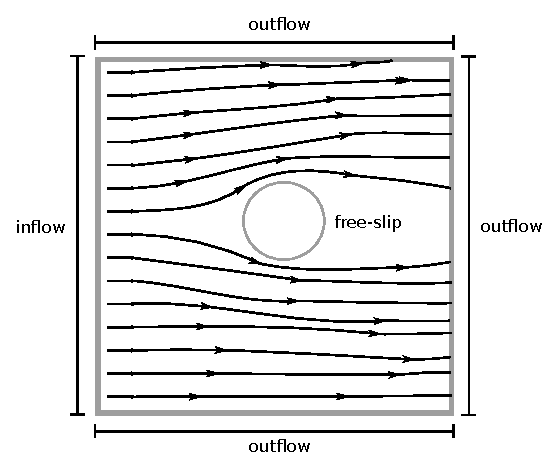
\includegraphics[width=8cm]{images/boundary_types}
\caption{Strömungslinien einer Beispielsimulation mit 3 verschiedenen Randbedingungen.}
\label{fig:stam_boundary_types}
\end{figure}

In der Simulation soll ein Teilbereich der echten Welt simuliert werden. Der
Wind wird von einigen Seiten künstlich in die Simulation gespeist. Dies nennt
man \PimiddyBegriff{inflow boundary} und ist eine Form der
Dirichlet-Randbedingung. Aus den verbleibenden Seiten soll der Wind frei aus der
Simulation \PimiddyQuotes{herausfließen}, als würde der Simulationsbereich dort
noch weitergeführt werden. Diese Art der Randbedingung nennt man
\PimiddyBegriff{outflow boundary}.

Simuliert man Rauch oder Wasser gibt es noch weitere Arten von Randbedingungen.
Die Grenze zwischen Wasseroberfläche und Luft nennt man \PimiddyBegriff{free
surface}-Randbedingung. Um diese umzusetzen müsste man $p=0$ außerhalb
des Wassers setzen. Diese Randbedingung wird hier nicht weiter beachtet.

Eine Zusammenfassung aller Randbedingungen ist in \autoref{fig:stam_boundary_types} zu sehen.

\subsubsection{Randbedingungen in der Simulation}

Es werden zuerst die Randbedingungen für die Hindernisse betrachtet. Hier sollen
\emph{free-slip}-Bedingungen erzwungen werden. Dies soll nicht explizit
hergeleitet werden, es werden nur die Veränderungen am Jacobiverfahren
beschrieben.

Im bisher beschriebenen Jacobiverfahren betrachtet man jede Zelle $p_{i,j,k}$
des Gitters und bilden die Summe über alle Nachbarzellen. Um die Randbedingungen
einfließen zu lassen, testet man, ob die Nachbarzelle von einem Hindernis
ausgefüllt ist (hier benutzen wir das Hindernisfeld $b_{i,j,k}$, was eingangs
beschrieben wurde). Gehört die Zelle zu einem Hindernis, wird nicht der
Druckwert der \emph{Nachbarzelle} zur Summe addiert, sondern der Wert der
\emph{aktuellen Zelle} (siehe \autoref{fig:stam_modified_jacobi_algorithm}
\PimiddyTodo{Wieso kann ich hier nur auf die subfigure verweisen?}). Auf
diese Weise kommt es zu keinem Druckunterschied in Richtung eines Hindernisses,
der Gradient in dieser Richtung ist also 0.  Algorithmus
\autoref{alg:stam_modified_jacobi_algorithm} zeigt den modifizierten
Algorithmus.

\begin{algorithm}
\caption{Der modifizerte Jacobi-Algorithmus}
\begin{algorithmic}
\Function{jacobi}{$p,x$}
	\State $p' = 0$
	\Comment{Ergebnisfeld ist $p'$}
	\ForAll{$(i,j,k)$}
		\State $\textrm{sum } \gets 0$
		\ForAll{Nachbarn $(i',j',k')$ von $p_{i,j,k}$}
			\If{$b_{i',j',k'} = 1$}
				\State $\textrm{sum} \gets \textrm{sum} + p_{i,j,k}$
			\Else
				\State $\textrm{sum} \gets \textrm{sum} + p_{i',j',k'}$
			\EndIf
		\EndFor
		\State $\textrm{new} = (\textrm{sum} - x_{i,j,k})/6$
		\State $p_{i,j,k}' \gets (1-\omega) \cdot p_{i,j,k} + \omega \cdot sum$
		\Comment{Gewichtete Jacobi-Iteration}
	\EndFor
	\State \Return $p'$
\EndFunction
\end{algorithmic}
\label{alg:stam_modified_jacobi_algorithm}
\end{algorithm}

\begin{figure}[ht]
\centering
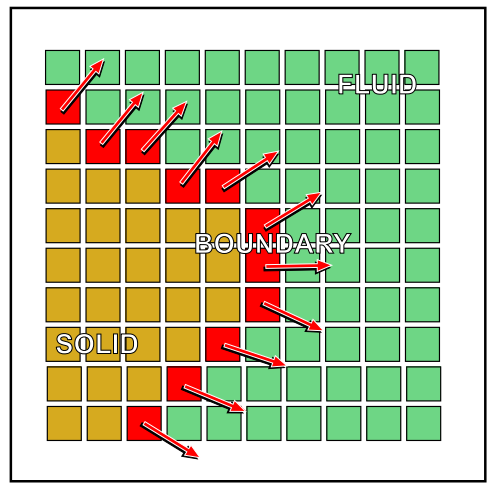
\includegraphics[width=6cm]{images/boundary_with_normals}
\caption{Hindernisse mit zugehöriger Normale}
\label{fig:stam_boundary_with_normals}
\end{figure}

Der Jacobi-Algorithmus löst die Poissongleichung allerdings nur annähernd.
Folglich werden auch die Randbedingungen nur annähernd gelöst. Dies kann im
nächsten Simulationsschritt zu Problemen führen. Daher wird in der
Implementierung die free-slip-Randbedingung nach dem Projektionsschritt
erzwungen (also nachdem der Gradient des Drucks vom Geschwindigkeitsfeld
subtrahiert wurde).

Idealerweise bräuchten wir dazu noch ein Feld $\vec{n}_{i,j,k}$, was in jedem
Punkt die Normale des Hindernisses angibt (siehe
\autoref{fig:stam_boundary_with_normals}). Dies wurde in einigen
Arbeiten umgesetzt (z.\,B. \cite{Bordignon}), es gibt jedoch eine Vereinfachung,
die dieses Feld nicht benötigt: Man iteriert erneut über alle
Gitterzellen und testet indem für jede Gitterzelle $(i,j,k)$, welche
Nachbarzellen von einem Hindernis ausgefüllt sind. Die zugehörige
Komponente der Geschwindigkeit $\vec{u}_{i,j,k}$ wird dann auf 0
gesetzt, siehe \autoref{alg:stam_enforce_free_slip}.

Für die outflow-Randbedingungen am Simulationsrand wird jede Randseite der
Simulation einzeln betrachtet. Die Geschwindigkeit einer Randzelle wird ersetzt
durch die Geschwindigkeit der \PimiddyQuotes{nächstinneren} Zelle.
Beispielsweise werden die Geschwindigkeitswerte $\vec{u}_{0,j,k}$ (also die an
der linken Simulationsseite) ersetzt durch die Werte $\vec{u}_{1,j,k}$. Analoges
wird für die anderen Seiten des Kubus getan, allerdings nicht dort, wo
inflow-Randbedingungen bestehen, wo also Wind in die Simulation hineinfließt.
Dadurch ergibt sich am Rand die Divergenz 0, der Druck ist hier also auch
annähernd 0 \PimiddyTodo{stimmt das überhaupt?}.

\begin{figure}[ht]
	\begin{subfigure}[b]{0.5\textwidth}
		\centering
		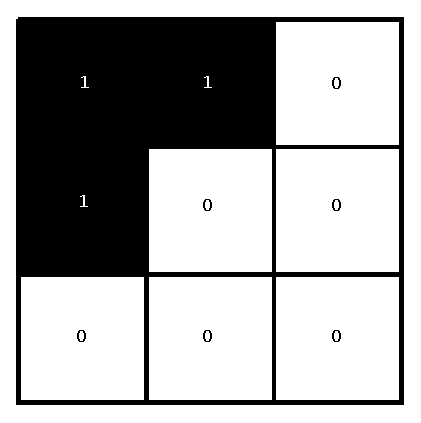
\includegraphics[width=\textwidth]{images/boundary_field_for_pressure}
		\caption{Ein beispielhaftes Hindernisfeld $b_{i,j}$}
	\end{subfigure}
	~
	\begin{subfigure}[b]{0.5\textwidth}
		\centering
		\def\svgwidth{\textwidth}
		\input{images/pressure_boundary.eps_tex}
		\caption{Die in die Druckberechnungen einfließenden Werte.}
	\label{fig:stam_modified_jacobi_algorithm}
	\end{subfigure}
\end{figure}

\begin{algorithm}
\caption{Die abschließende Randbedingungserzwingung}
\begin{algorithmic}
\Function{FreeSlipBoundary}{$\vec{v},b$}
	\ForAll{$(i,j,k)$}
		\If{$b_{i-1,j,k} = 1$ or $b_{i+1,j,k} = 1$}
			\State $\vec{u}_{i,j,k}^x = 0$
		\EndIf
		\If{$b_{i,j-1,k} = 1$ or $b_{i,j+1,k} = 1$}
			\State $\vec{u}_{i,j,k}^y = 0$
		\EndIf
		\If{$b_{i,j,k+1} = 1$ or $b_{i,j,k-1} = 1$}
			\State $\vec{u}_{i,j,k}^z = 0$
		\EndIf
	\EndFor
\EndFunction
\end{algorithmic}
\label{alg:stam_enforce_free_slip}
\end{algorithm}

\section{OpenCL}
\label{sec:opencl}

\subsection{Einleitung}

In diesem Abschnitt wird OpenCL als das Framework, welches für die Berechnungen
verwendet wurde, vorgestellt. Dabei wird im ersten Teil zunächst eine kurzer
geschichtlicher Abriss gegeben und die Stellung von OpenCL unter anderen
Frameworks herausgestellt. Im Anschluss wird der Begriff Parallelität definiert
und speziellere Ausprägungen davon im Kontext mit OpenCL besprochen. Mit diesem
Wissen lässt sich abschätzen, wieso die vorgestellten Algorithmen sich besonders
für eine parallele Abarbeitung eignen.

Im nächsten Abschnitt wird die Architektur von OpenCL im Detail vorgestellt,
wobei für die für die Arbeit irrelevanten Teile nur angeschnitten werden.

Schließlich wird ein vollständiges Programm vorgestellt, welches eine einfache
Berechnung in OpenCL durchführt. Dies soll vor allem den in der Implementierung
immer wiederkehrenden Arbeitsablauf deutlich machen, der nötig ist, um Daten und
Programme auf der GPU zu verwalten. Im Kapitel über die konkret implementierten
Algorithmen wird dann nur noch der OpenCL-C-Code beschrieben.

\subsection{Geschichtliches}

Strömungsmechanische Berechnungen gelten als sehr rechenaufwändiges
Problem, für das traditionell große Rechencluster eingesetzt werden.
Diese Cluster bestehen üblicherweise aus tausenden einzelnen
Prozessoren, die jeweils einen kleinen Teil des Problems lösen, zum
Beispiel nur einen Ausschnitt des Definitionsbereichs berechnen. Alle
Prozessoren werden zu einem 3D-Gitter zusammengefasst und decken so
den gesamten Simulationsbereich ab. Dadurch, dass die Recheneinheiten
parallel arbeiten können, erhält man schnell eine Lösung des Problems.

Desktop-Rechner hatten bis vor einigen Jahren allerdings nur einen
einzelnen Prozessor zum Rechnen verbaut, sodass die oben beschriebene
Arbeitsweise nicht übertragbar war. Tatsächlich zeigte sich bei
Desktop-CPUs bis ca.\,2005 ein Anstieg in der Taktrate der
Prozessoren, aber nicht deren Anzahl\PimiddyTodo{Tabelle mit Anstieg
der Taktrate einbauen}. Diese Entwicklung endete allerdings, da mit
der Taktrate auch der Stromverbrauch immer weiter ansteigt. In
\cite{Chandrakasan1995} findet sich der folgende Zusammenhang zwischen
dem Stromverbrauch in Watt $P$, der Taktfrequenz $f$, der Spannung $V$ und
des Widerstands $C$ eines Prozessors:

\begin{align}
P = C V^2 f
\end{align}

Ersetzt man einen einzelnen Prozessor mit Taktfrequenz $f$, Spannung
$V$ und Widerstand $C$ durch zwei Prozessoren halber Frequenz $f/2$,
so erhöht sich laut \cite{Chandrakasan1995} zwar der Widerstand auf
$2.2C$, aber die Spannung sinkt drastisch auf $0.6V$. Die zwei
Prozessoren verbrauchen daher zusammen nur 0.396 mal so viel Leistung
wie der einzelne Prozessor. Aufgrund dessen geht aktuell der Trend hin
zu Prozessoren mit mehreren Kernen (momentan bis zu 8).

In den letzten Jahren ist auch die Leistungsfähigkeit von
Grafikprozessoren (GPUs) rasant angestiegen (siehe
\autoref{fig:opencl_gflops_gpu_vs_cpu} und
\autoref{fig:opencl_gbs_gpu_vs_cpu}). GPUs waren anfangs spezialisierte Recheneinheiten, um die in
\autoref{sec:opengl} vorgestellte Grafikpipeline umzusetzen. Da jeder
Vertex und jedes Fragment für sich bearbeitet werden kann, bot sich
hier von Anfang an eine hochparallele Architektur an.

\begin{figure}
	\begin{subfigure}[t]{0.5\textwidth}
		\centering
		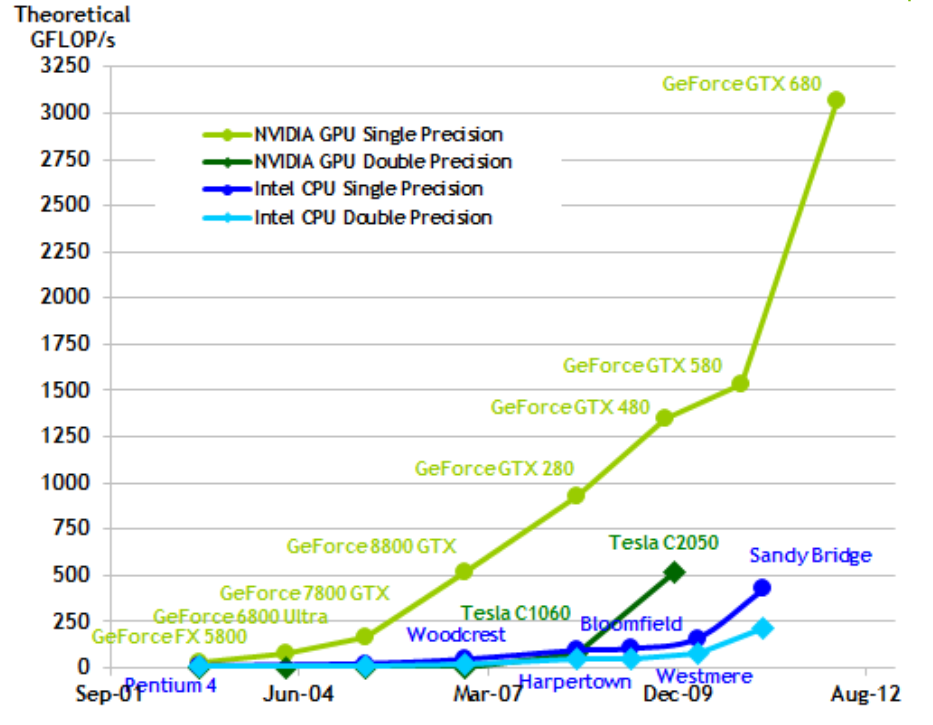
\includegraphics[width=\textwidth]{images/gflops_cpu_vs_gpu}
                \caption{Anstieg der Gigaflops pro Sekunde im Vergleich zwischen CPUs und GPUs}
		\label{fig:opencl_gflops_gpu_vs_cpu}
	\end{subfigure}
	~
	\begin{subfigure}[t]{0.5\textwidth}
		\centering
		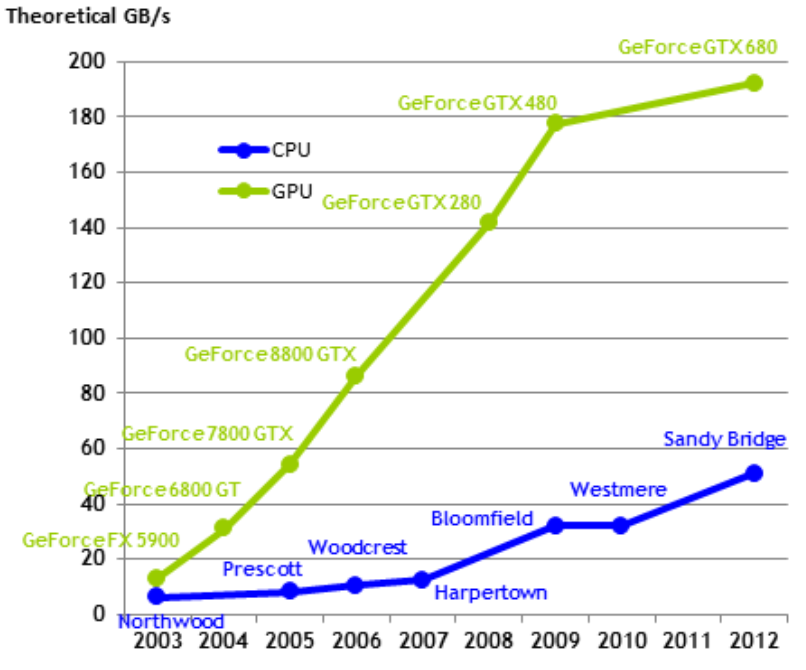
\includegraphics[width=\textwidth]{images/gbs_cpu_vs_gpu}
                \caption{Anstieg der Bandbreite im Vergleich zwischen CPUs und GPUs}
		\label{fig:opencl_gbs_gpu_vs_cpu}
	\end{subfigure}
        \caption{Vergleich zwischen CPUs und GPUs}
\end{figure}

Mit der Zeit stieg aber die Nachfrage nach mächtigeren Shaderprogrammen, um
aufwändigere Grafikeffekte umzusetzen. Daher wurden die Recheneinheiten der GPUs
immer weiter verallgemeinert. Mit Hilfe dieser leistungsfähigen Shaderprogramme
begannen auch Wissenschaftler, Grafikkarten für Rechenaufgaben zu verwenden und
es entstanden \Pimiddyca 2004 erste Umsetzungen von Stams Methode auf
Grafikkarten\cite{Wu2004}.

Allerdings war es bis dato weder möglich, rohen Speicher auf der
Grafikkarte zu reservieren, noch beliebige Programme zu starten, die
auf diesem Speicher arbeiten. Vielmehr mussten die bestehenden
Mechanismen der Grafikpipeline \PimiddyQuotes{missbraucht} werden. So
wurden Simulationsergebnisse in zweidimensionalen Texturen
gespeichert, die man als \PimiddyQuotes{Rendertargets} angeben
konnte. Dann wurde ein Rechteck auf den Bildschirm gezeichnet, um die
Ausführung der Berechnungs-Shader künstlich anzustoßen.

Um komfortabler allgemeine Berechnungen auf der Grafikkarte bzw. auf
Mehrkernsystemen zu tätigen, wurden mehrere Frameworks entwickelt,
unter anderem CUDA von NVidia und AMDs Stream Framework. Diese waren
aber nicht formal spezifiziert und oft herstellerabhängig. Ein
CUDA-Programm ist \PimiddyzB nur auf GPUs von NVidia lauffähig.

Als Lösung für dieses Problem wurde Ende 2008 das OpenCL-Framework in
der Version 1.0 veröffentlicht, unterstützt von unter anderem Apple,
NVidia, AMD und IBM. OpenCL ermöglicht das Erstellen von parallel
laufenden Programmen auf GPUs, CPUs und sogar FPGAs. Man spricht
allgemein von \PimiddyBegriff{heterogenen Systemen}. Inzwischen ist
OpenCL bei Version 1.2 angelangt, wobei diese noch nicht von allen
Herstellern unterstützt wird.

\subsection{Arten der Parallelität}

Ob ein Problem mit Hilfe einer Grafikkarte gut lösbar ist, hängt vor allem davon
ab, ob es gut \emph{parallelisierbar} ist. Es soll daher in diesem Abschnitt der
Begriff Parallelität definiert werden. Außerdem sollen die verschiedenen
Ausprägungen von Parallelität, die OpenCL unterstützt, erläutert werden.
Schließlich wird begründet, wieso sich Stams Methode gut für die Berechnung mit
OpenCL eignet.

\emph{Parallelität} oder auch \emph{Nebenläufigkeit} liegt im
Allgemeinen vor, wenn mehrere Operationsströme unabhängig voneinander
in einem Zeitschritt fortschreiten können\cite{munshi2011}. Ein
klassisches Beispiel für nebenläufige Operationsströme bieten
\emph{Threads} in Programmiersprachen wie Java. Während ein Thread
beispielsweise auf Daten von einem Netzwerksocket wartet, kann ein
anderer einen Ladebalken anzeigen. Mit Hilfe von Threads können sowohl
gleiche Bereiche des Codes mehrfach parallel ausgeführt werden
(\PimiddyzB eine bestimmte Funktion mit verschiedenen Eingaben) oder
auch vollkommen verschiedene Bereiche.

In OpenCL werden insgesamt zwei Arten von Parallelität unterschieden:
\PimiddyBegriff{Taskparallelität} und
\PimiddyBegriff{Datenparallelität}. Der Unterschied liegt darin, dass
entweder mehrere \emph{Aufgaben} (Tasks) auf die nebenläufigen
Operationsströme verteilt werden oder mehrere \emph{Datenblöcke}.

Die oben genannten Threads werden meistens für taskparallele Probleme
eingesetzt. Hierbei wird ein Problem in mehrere Aufgaben unterteilt,
die möglichst unabhängig voneinander auf den Recheneinheiten
ausgeführt werden können und eventuell auch unabhängig voneinander
Ergebnisse produzieren. Die Operationsströme und die Eingangsdaten der
verschiedenen parallel laufenden Einheiten sind eventuell sehr
unterschiedlich voneinander.

Bei einem \emph{datenparallelen} Problem hingegen wendet man denselben
Operationsstrom (dasselbe Programm) auf jeweils unterschiedliche
Eingabedaten an. Das einfachste Beispiel für Datenparallelität ist
\emph{Single Instruction Multiple Data} (SIMD), wo das Programm meist aus
einer einzigen Operation besteht. Die Addition zweier Arrays ist
beispielsweise ein Problem, das auf diese Weise lösbar ist. Für jedes
Arrayelement wird ein Prozessor verwendet, der folglich nur Logik für
die Addition zweier Zahlen benötigt. Die nebenläufig arbeitenden
Prozesse beeinflussen sich in diesem Beispiel nicht gegenseitig. Dies
ist aber nicht zwingend für ein datenparalleles Problem, und OpenCL
unterstützt auch Synchronisationsmechanismen. Aufwändigere
datenparallele Probleme enthalten \PimiddyInlineCode{if}-Abfragen und
können so unterschiedliche Ausführungspfade je nach Eingabedaten
nehmen. Diese Art der Parallelität nennt man \emph{Single Program
Multiple Data} (SPMD)\cite{Mattson:2004:PPP:1406956}.

Grafikkarten sind aus historischen Gründen sehr gut für datenparallele
Probleme geeignet, denn die Umsetzung der Grafikpipeline stellt
ebenfalls ein solches Problem dar.

Die Funktionen in Stams Verfahren sind alle datenparallel
gestaltet. Als Eingabe dient immer ein dreidimensionales Vektor- oder
Skalarfeld, bei dem jeder Voxel für sich bearbeitet werden kann (unter
Zuhilfenahme seiner Nachbarschaft im Eingabefeld), wodurch wieder ein
Vektor- bzw. Skalarfeld entsteht. Auch das später vorgestellte
Partikelsystem ist ein datenparalleles Problem, denn jede Schneeflocke
kann für sich bearbeitet werden (Flocken beeinflussen sich nicht
gegenseitig im hier gewählten Modell).

\subsection{Architektur}

Die OpenCL-Architektur ist in 4 Teile geteilt, die nun separat
erläutert werden sollen:

\begin{enumerate}
\item Das \PimiddyBegriff{Platform-Model} bietet eine abstrakte
Beschreibung eines heterogenen Systems. Hier wird der
\PimiddyBegriff{Host} als Steuereinheit sowie die Arten der
Komponenten wie Grafikkarten, CPUs und integrierte Chips definiert.
\item Das \PimiddyBegriff{Execution-Model} beschreibt den Begriff
\PimiddyBegriff{Kernel} als ein Programm, das auf dem Device ausgeführt wird, sowie die
Mechanismen um Kernel zu starten und auszuführen.
\item Das \PimiddyBegriff{Memory-Model} beschreibt die unterschiedlichen Speichertypen, die
OpenCL bereitstellt.
\item \PimiddyBegriff{OpenCL-C} stellt momentan die einzige Sprache
dar, mit der parallele Programme in OpenCL verfasst werden können.
\end{enumerate}

\subsubsection{Platform-Model}

OpenCL soll sowohl auf CPUs als auch auf GPUs und sogar
\PimiddyQuotes{exotischeren} Systemen wie FPGAs eingesetzt
werden. Daher müssen als Basis allgemeine Begriffe zur Beschreibung
von Systemen mit mehreren Prozessoren und Komponenten definiert
werden. Dies geschieht im Platform-Model.

OpenCLs Platform-Model ist in \autoref{fig:opencl_platform_model}
dargestellt. Es ist sehr allgemein gehalten, sodass es sich auf eine
Vielzahl von Hardwaresystemen sinnvoll übertragen lässt. Im Modell
existiert genau einen \PimiddyBegriff{Host}, der mehrere
\PimiddyBegriff{Devices} verwaltet. Ein Device ist zum Beispiel eine
Grafikkarte oder eine CPU. Ein typisches Desktopsystem als Host könnte
beispielsweise drei Devices enthalten: eine CPU und zwei Grafikkarten.

Ein Device hat mehrere \PimiddyBegriff{Compute Units} (CU), die
wiederum \PimiddyBegriff{Processing Elements} (PE) enthalten. Die
eigentlichen Berechnungen finden auf den Processing Elements
statt. Auf einer CU laufen meistens mehrere PE parallel und
kommunizieren gegebenenfalls miteinander über CU-eigenen Speicher und
Synchronisationspunkte. Die Unterscheidung zwischen CU und PE muss auf
Hardware-Ebene allerdings nicht vorhanden sein, sie ist aber dennoch
für das Execution-Model wichtig (siehe unten).

Eine Grafikkarte hingegen besitzt im allgemeinen wesentlich mehr
Compute Units und Processing Elements.

\begin{figure}[ht]
\centering
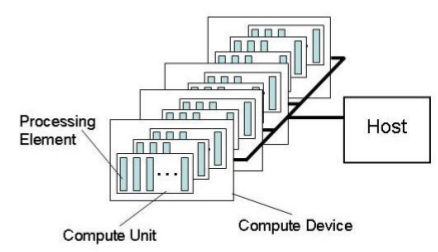
\includegraphics[width=14cm]{images/opencl_platform_model}
\caption{Platform-Model in OpenCL}
\label{fig:opencl_platform_model}
\end{figure}

\subsubsection{Execution-Model}
\label{sec:opencl_execution_model}

Eine OpenCL-Anwendung wird gesteuert durch das Host-Program (das auf
dem Host läuft). Das Host-Programm ist in einer Programmiersprache wie
Java oder C++ geschrieben und ist zuständig für die Reservierung von
Speicher auf den Devices, das Abfragen von Device-Eigenschaften und
dem Starten der sogenannten \PimiddyBegriff{Kernel}.

Kernel sind Programme, die auf dem Device ausgeführt werden und somit
die eigentliche parallel ausgeführte Logik enthalten. Sie erhalten vom
Host-Programm die vorher reservierten Speicherbereiche auf dem Device,
sowie weitere Parameter. Ansonsten verhalten sie sich ähnlich einer
freien Funktion in einer normalen Programmiersprache. Sie können den
Speicher des Devices, auf dem sie ausgeführt werden, sowohl lesen als
auch schreiben und sind so in der Lage, Ergebnisse zu produzieren.

\PimiddyListingRef{lst:opencl_add_arrays_example} zeigt einen in
OpenCL-C geschriebenen Kernel, der zwei Elemente aus den Arrays
\PimiddyInlineCode{a} und \PimiddyInlineCode{b} addiert und das
Ergebnis in ein Array \PimiddyInlineCode{result} zurückschreibt. An
diesem Beispiel zeigt sich bereits, dass OpenCL auf datenparallele
Probleme zugeschnitten ist: Der Kernel schreibt nur ein einzelnes
Arrayelement mit Index \PimiddyInlineCode{i} zurück. Das gesamte Array
wird dadurch bearbeitet, dass man den Kernel mehrfach (parallel) mit
unterschiedlichen Indizes instanziiert. Das Execution-Model legt fest,
wie Kernel parallel auf einem Device \emph{ausgeführt} und
\emph{gestartet} werden. Wie Kernel \emph{geschrieben} werden, wird
hingegen im Abschnitt über OpenCL-C erklärt.

\begin{listing}
    \begin{minted}[frame=lines]{c}
kernel void add_arrays(
    global float const *a,
    global float const *b,
    global float *result)
{
  // Gibt die ID der aktuellen Instanz des Kernels zurueck,
  // siehe unten.
  size_t i = get_global_id(0);
  result[i] = a[i] + b[i];
}
    \end{minted}
    \caption{Ein Beispiel-Kernel zum Addieren zweier Arrays.}
    \label{lst:opencl_add_arrays_example}
\end{listing}

Bei der folgenden Erklärung werden alle Mechanismen weggelassen, die
mit Taskparallelität zusammen hängen, da diese Art der Parallelität in
dieser Arbeit keine Rolle spielt.

Um einen Kernel wie den obigen auszuführen, werden neben dem Namen des
Kernels die folgenden Daten angegeben:

\begin{itemize}
\item Das Gerät, auf dem der Kernel ausgeführt werden soll.
\item Eine $n$-dimensionale \PimiddyBegriff{globale Arbeitsgröße} $\mathcal{G}$.
\item Eine optionale $n$-dimensionale \PimiddyBegriff{lokale Arbeitsgröße} $\mathcal{L}$.
\item Benutzerdefinierte Eingabedaten (reservierte Speicherbereiche, Parameter).
\end{itemize}

Die globale Arbeitsgröße bestimmt, wie viele Instanzen des gegebenen
Kernels \emph{insgesamt} gestartet werden. Es wird damit allerdings
noch nichts darüber ausgesagt, wie viele Instanzen gleichzeitig
\emph{parallel} ausgeführt werden. Man kann ein-, zwei-, oder
dreidimensionale Arbeitsgrößen angeben.

Um mit dem Kernel aus
\PimiddyListingRef{lst:opencl_add_arrays_example} das
\PimiddyInlineCode{result}-Array komplett zu füllen, müsste man also
$\mathcal{G}=\PimiddyFormelText{Länge}(\texttt{result})$ wählen (also eine
eindimensionale Arbeitsgröße). Das Device startet dann entsprechend
viele \emph{Instanzen} des Kernels, die auch
\PimiddyBegriff{Work-Items} genannt werden. Jedes Work-Item steht für
sich und führt den Code aus, den der Kernel vorgibt. Zusätzlich zu den
Eingabedaten, die vom Benutzer angegeben werden, erhält ein Work-Item
weitere Parameter, darunter seine eindeutige \emph{globale ID}. Sie
beginnt im Beispiel bei $0$ und geht bis einschließlich
Länge$(\texttt{result})-1$. Im allgemeinen ist die ID $n$-dimensional
und richtet sich danach, was für $\mathcal{G}$ angegeben wurde. Die
globale ID wird im Code häufig als Index in ein Array benutzt. Da sie
eindeutig ist, gibt es auf diese Weise keine Konflikte mit anderen,
parallel laufenden Work-Items, die auch in das Array schreiben.

Oftmals reicht diese Form der Ausführung aus, grade wenn die
Work-Items untereinander nicht miteinander kommunizieren
müssen. Intern fasst das Device allerdings mehrere Work-Items zu
\PimiddyBegriff{Work-Groups} zusammen. Die Besonderheit bei
Work-Groups ist, dass die darin enthaltenen Work-Units auf derselben
\emph{Compute Unit} ausgeführt werden. Dies hat zweierlei
Konsequenzen:

\begin{enumerate}
\item Die Work-Items einer Work-Group können über \PimiddyBegriff{lokalen
Speicher} (siehe den Abschnitt zum Memory-Model) auf der CU Daten
untereinander austauschen. Dies kann als Cache-Mechanismus sehr nützlich
sein, denn der CU-interne Speicher ist wesentlich schneller als der
sonst zur Verfügung stehende globale Speicher.
\item Die Work-Items können sich gegeneinander mit Hilfe von Barrieren
beeinflussen. Beispielsweise könnten an einer Stelle im Code alle
Work-Items aufeinander warten und dann erst gemeinsam weiter fortfahren.
\end{enumerate}

Man kann die Größe der Arbeitsgruppe bei der Ausführung auch explizit
angeben, muss aber darauf achten, dass die Arbeitsgruppengröße in
jeder Dimension durch die globale Arbeitsgröße teilbar ist. Gibt man
die Arbeitsgruppengröße nicht an, wählt die OpenCL-Implementierung
eine angemessene Größe aufgrund einer Heuristik. Jedes Work-Item
erhält vom Device zusätzlich zu seiner globalen ID immer eine
\emph{lokale ID}, die das Item innerhalb seiner Work-Group eindeutig
identifiziert. Außerdem kann ein Work-Item seine \emph{group ID}
abfragen. Im Übrigen ist nicht garantiert, dass die Work-Items einer
Work-Group parallel ausgeführt werden.

\begin{figure}[ht]
\centering
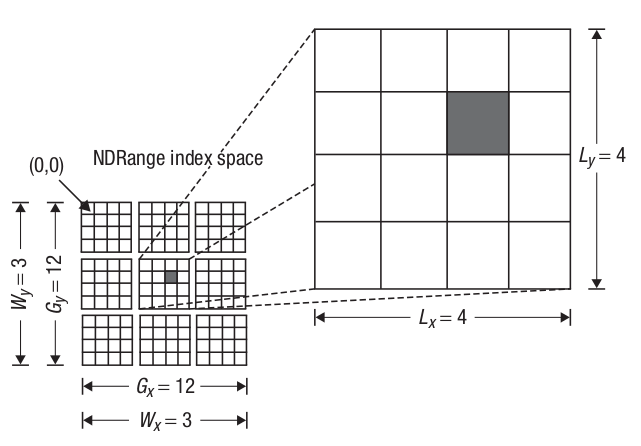
\includegraphics[width=13cm]{images/execution_model}
\caption{Beispiel zur Ausführung eines Kernels. Die globale Arbeitsgröße ist $(12,12)$, die Arbeitsgruppengröße ist $(4,4)$, es entstehen also $3 \times 3$ Gruppen. Jedes Work-Item erhält eine lokale ID (im Bild markiert $(2,1)$) und eine globale ID (im Bild markiert $(6,5)$).}
\label{fig:opencl_execution_model}
\end{figure}

\subsubsection{Memory-Model}
\label{sec:opencl_memory_model}

Da OpenCL auf vielen verschieden Systemen lauffähig sein soll, müssen
-- ähnlich wie beim Platform-Model -- allgemeine Begriffe geschaffen
werden, welche die für den Benutzer verfügbaren Speicherbereiche
beschreiben.

Es gibt zwei Arten von Speicherobjekten in OpenCL:
\PimiddyBegriff{buffer objects} und
\PimiddyBegriff{image objects}. \PimiddyEnglBegriff{Buffer objects} stellen rohe
Speicherblöcke einer bestimmten Größe dar, die der Anwender mit
beliebigem Inhalt füllen kann. Sie sind in allen Implementierungen
verfügbar und nur durch den verfügbaren Speicher begrenzt.

\PimiddyEnglBegriff{Image objects} hingegen sind zur Speicherung von zwei- und
dreidimensionalen Bildern gedacht. Sie haben ihren Platz in OpenCL
gefunden, da GPUs spezielle Hardware zur Adressierung von Bildern
enthalten, auf die man in OpenCL aus Performancegründen eventuell
zurückgreifen will. Beim Erstellen eines \PimiddyEnglBegriff{image object} gibt man seine
Größe und das gewünschte Format an, wobei nicht alle theoretisch
verfügbaren Formate von allen Geräten unterstützt werden und die Größe
beschränkt ist. Beim Zugriff auf ein Bild muss man den Adressierungs-,
und den Filtermodus angeben, sowie die Koordinaten des Bildpunktes,
den man laden will. Es ist auch möglich, mit einer
Fließkommakoordinate auf ein Bild zuzugreifen. In diesem Fall bestimmt
der Filtermodus, wie Werte zwischen den Bildpunkten interpretiert
werden. Ein Device muss nicht zwingend \PimiddyEnglBegriff{image objects}
unterstützen. Außerdem sind dreidimensionale Texturen sind nicht aus
Kerneln heraus beschreibbar (zweidimensionale schon).

Des weiteren gibt es 5 verschiedene \emph{Speicherbereiche} in OpenCL:

\begin{description}
\item[Hostspeicher] Diese Art Speicher ist nur für das Host-Programm
verfügbar.
\item[Globaler Speicher] Auf diesen Speicherbereich können alle
Work-Items sowohl lesend als auch schreibend zugreifen. Der Zugriff
kann zudem wahlfrei geschehen, wobei Lesezugriffe je nach Device
gecached sein können. Die Zugriffszeit ist ansonsten stark davon
abhängig, wie auf den Speicher innerhalb einer Work-Group zugegriffen
wird.
\item[Konstanter Speicher] Dieser Speicherbereich bleibt während die
Ausführung eines Kernels konstant. Er wird am Anfang einmal
geschrieben und steht allen Work-Items danach nur lesend zur
Verfügung. Zugriff auf den konstanten Speicher ist allerdings sehr
performant.
\item[Lokaler Speicher] Auf diesen Speicherbereich können alle
Work-Items innerhalb einer Work-Group lesen und schreibend
zugreifen. Im Allgemeinen ist der Zugriff sehr schnell, da der
Speicher oft auf der CU verbaut ist.
\item[Privater Speicher] Dieser Speicherbereich ist nur für das
aktuelle Processing Element verfügbar und enthält unter anderem lokale
Variablen.
\end{description}

\autoref{fig:opencl_memory_model} zeigt alle Speichertypen im
Überblick. Es ist erkennbar, dass das Host-Programm lediglich den
konstanten und den globalen Speicher lesen und schreiben kann. Da der
Transfer von Host-Speicher zu Device-Speicher allerdings
vergleichsweise langsam vonstatten geht, wird im Allgemeinen versucht,
wenige Speichertransfers durchzuführen und auf dem Device zu bleiben.

Um ein \PimiddyEnglBegriff{buffer object} zu erzeugen, ruft das Host-Programm die Funktion
\PimiddyInlineCode{clCreateBuffer} auf und übergibt:

\begin{itemize}
\item die Größe des Buffers in Bytes
\item das Device, auf dem der Buffer erstellt werden
soll\PimiddyFootnote{hier wird auf die Einführung des
\PimiddyBegriff{Kontext} verzichtet und nur vom Device gesprochen.}
\item Flags, die angeben, ob der Buffer für die Kernel lesbar oder
auch schreibbar sein soll
\item Optional der initiale Inhalt des Buffers
\end{itemize}

Um einen Buffer vom Host-Programm aus zu schreiben oder auszulesen,
kann man den Inhalt des Buffers mit dem Kommando
\PimiddyInlineCode{clEnqueueMapBuffer} auf einen Speicherbereich des
Host-Speichers übertragen. Nachdem man aus diesem Bereich gelesen oder
in den Bereich geschrieben hat, muss man ihn mit
\PimiddyInlineCode{clEnqueueUnmapBuffer} wieder freigeben. Bei einer
Schreiboperation wird der Buffer daraufhin wieder zum Device übertragen.

Um ein (zweidimensionales) \PimiddyEnglBegriff{image object} zu erstellen, ruft man die Funktion
\PimiddyInlineCode{clCreateImage2D} auf und übergibt die folgenden Parameter:

\begin{itemize}
\item die Breite und Höhe des Bildes
\item das Format, zum Beispiel \PimiddyInlineCode{CL\_RGB, CL\_FLOAT} für ein Bild mit drei \PimiddyInlineCode{float}-Farbkanälen
\item Flags, die angeben, ob das Bild nur lesbar oder auch schreibbar sein soll (analog zu \PimiddyEnglBegriff{buffer objects})
\item Optional der initiale Inhalt des Bildes
\end{itemize}

Analog zu \PimiddyEnglBegriff{buffer objects} gibt es Kommandos, um den Inhalt von und zum Host zu übertragen.

\begin{figure}[ht]
\centering
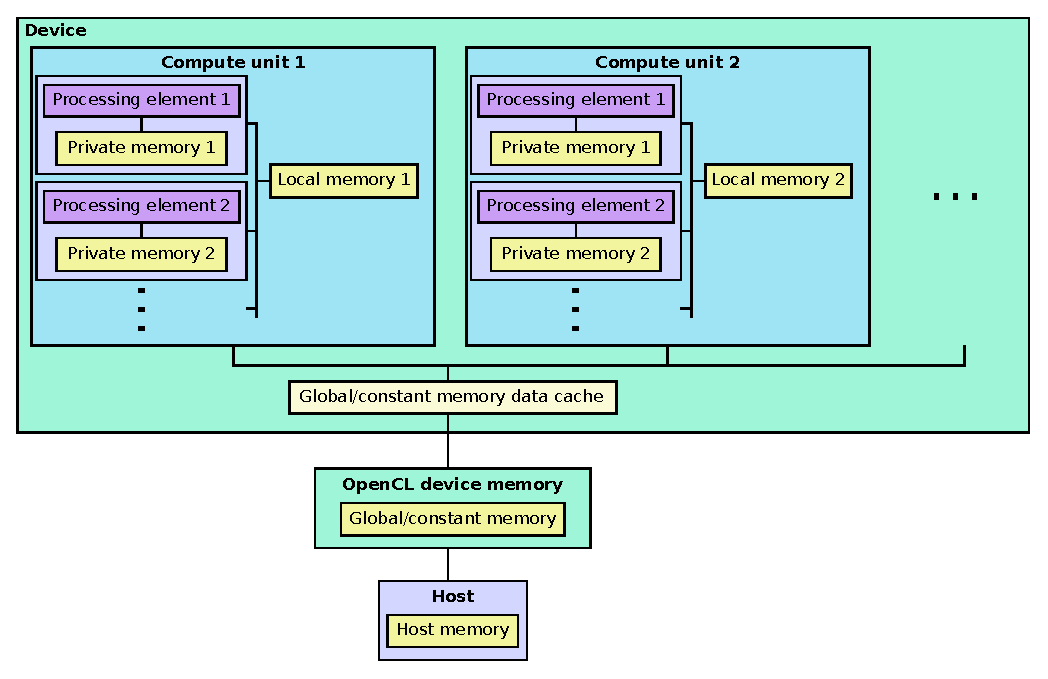
\includegraphics[width=15cm]{images/opencl_memory_model}
\caption{Ein Überblick über die verschiedenen Speicherbereiche, die OpenCL vorgibt, und der Zusammenhang mit dem Execution-Model.}
\label{fig:opencl_memory_model}
\end{figure}

Es ist außerdem möglich, Speicher zwischen OpenGL und OpenCL zu
teilen, sowohl für image-, als auch \PimiddyEnglBegriff{buffer objects}. Dies wird unter
anderem beim Partikelsystem für die Schneeflocken dazu verwendet, die
Eigenschaften der Schneeflocke wie die Position direkt im
OpenGL-Vertexbuffer zu verändern. Es werden so Speicherplatz und
Kopierkosten gespart. Allerdings muss sichergestellt sein, dass alle
OpenCL-Operationen auf dem entsprechenden Buffer abgeschlossen sind,
bevor der Buffer von OpenGL verwendet werden kann. Der umgekehrte
Fall, also der Abschluss aller OpenGL-Operationen auf dem Buffer, muss
auch sichergestellt werden. Dies ist momentan nur möglich, indem man
die Kommandos \PimiddyInlineCode{glFinish} und
\PimiddyInlineCode{clFinish} verwendet. Diese schließen allerdings
global alle noch laufenden Operationen auf \emph{allen} Buffern ab und
blockieren solange das Hauptprogramm. Es kann daher zu
Performanceproblemen kommen.

\subsubsection{OpenCL-C}

In diesem Abschnitt wird die Programmiersprache OpenCL-C eingeführt,
sowie die Zusammenhänge zu den vorher besprochenen Abschnitten
deutlich gemacht. Es soll dabei zunächst der Weg vom fertig
geschriebenen OpenCL-C-Programmtext zu seiner Ausführung auf einem
Device deutlich gemacht werden. Bei den Erklärungen wird
zwischen dem Host-Programm und dem OpenCL-C-Programm hin- und
hergesprungen. Dabei ist zu beachten, dass die von der OpenCL-Runtime
bereitgestellten Funktionen immer mit
\PimiddyQuotes{\PimiddyInlineCode{cl}} beginnen. Diese Funktionen
werden also immer auf dem Host ausgeführt. Im Anschluss werden
einige Besonderheiten von OpenCL-C gegenüber C99 herausgestellt.

OpenCL-C ist momentan die einzige Programmiersprache, welche die
OpenCL-Spe\-zi\-fi\-ka\-ti\-on zur Erstellung von OpenCL-Kerneln formal
beschreibt. Sie basiert auf der ISO-genormten Sprache C99 (genauer
ISO/IEC 9899:1999), wobei einige sprachliche Erweiterungen und eine
große Standardbibliothek ergänzt wurden. Im Folgenden wird minimales
Grundwissen über C99 vorausgesetzt.

OpenCL-C-Programme werden entweder in separaten Textdateien
gespeichert und im Host-Programm in einen String geladen, oder sie
werden direkt im Host-Programm als Stringliteral eingebunden. Der
String mit dem Programmcode wird dann für ein bestimmtes
Device\PimiddyFootnote{Streng genommen ist es eine Liste von Devices.}
mit Hilfe der Funktionen \PimiddyInlineCode{clCreateProgramWithSource}
und \PimiddyInlineCode{clBuildProgram} kompiliert und es entsteht ein
\PimiddyBegriff{program object}. Beim Kompilieren lassen sich noch
Optimierungsflags angeben. Ein Beispiel soll die folgenden Erklärungen
verdeutlichen:

\begin{minted}[frame=lines]{c}
// Hilfsfunktion zum Quadrieren eines Werts.
// Achtung: Nicht von aussen aufrufbar!
float square(float x)
{
  return x*x;
}

// Quadriert ein Array und addiert eine Konstante.
kernel void square_and_add(
    global float *a,
    private float b)
{
  private float current_value = a[get_global_id(0)];
  a[get_global_id(0)] = helper(current_value) + b;
}

constant float4 null_value = (float4)(0.0f);

// Setzt alle Pixel eines 2D-Bildes auf 0 zurueck.
kernel void null_image(
    global write_only image2d_t bild)
{
  write_imagef(
    bild,
    (int2)(
        get_global_id(0),
        get_global_id(1)),
    (float4)(
        0.0f));
}
\end{minted}

Aus dem \PimiddyEnglBegriff{program object} lassen sich nun mittels
\PimiddyInlineCode{clCreateKernel} ein oder mehrere
\PimiddyBegriff{kernel object} erzeugen. In OpenCL-C sind Kernel
normale C99-Funktionen mit Rückgabetyp \PimiddyInlineCode{void}, die
mit dem Attribut \PimiddyInlineCode{kernel} ausgestattet sind. Nur
diese Funktionen können von außen als \PimiddyQuotes{Einsprungpunkte}
für die OpenCL-Runtime benutzt werden. Aus der Funktion
\PimiddyInlineCode{helper} im Programmcode oben kann \PimiddyzB kein
\PimiddyEnglBegriff{kernel object} erzeugt werden. Die Funktion
\PimiddyInlineCode{clCreateKernel} erhält das \PimiddyEnglBegriff{program object} und den
Namen des Kernels als Parameter.

Die Kernelfunktionen in OpenCL-C erhalten Parameter, die vom
Host-Programm vor der Ausführung des Kernels gesetzt werden
müssen. Die Funktion \PimiddyInlineCode{clSetKernelArg} erhält dazu das
\PimiddyEnglBegriff{kernel object}, den Index des Parameters, den man setzen will, sowie den
Parameter selber.

\PimiddyEnglBegriff{Buffer objects} werden in OpenCL-C als \emph{Pointer} repräsentiert. Die
Sprache sieht keine mehrdimensionalen Strukturen vor. Diese müssen
mittels Indextransformationen selber geschrieben werden. \PimiddyEnglBegriff{Image objects}
haben den speziellen Typ \PimiddyInlineCode{image2d\_t}
bzw. \PimiddyInlineCode{image3d\_t} und müssen mit
\PimiddyInlineCode{read\_only} bzw. \PimiddyInlineCode{write\_only}
qualifiziert werden (gleichzeitiger Lese-, und Schreibzugriff ist
aufgrund von Hardwarebeschränkungen nicht möglich). Zum Schreiben
steht die Funktion \PimiddyInlineCode{write\_imagef}, zum Lesen die
Funktion \PimiddyInlineCode{read\_imagef} zur Verfügung.

Sind alle Parameter gesetzt, kann man der Funktion
\PimiddyInlineCode{clEnqueueNDRangeKernel} das \PimiddyEnglBegriff{kernel object}, sowie die
in \autoref{sec:opencl_execution_model} beschriebenen Parameter
übergeben und der Kernel wird auf dem Device ausgeführt.

In OpenCL ist es wichtig, jede Variable mit einem Attribut
auszustatten, die den Speicherbereich der Variable angibt. Mit
Ausnahme des Hostspeichers gibt es für jeden der in
\autoref{sec:opencl_memory_model} beschriebenen Bereiche ein
Schlüsselwort: \PimiddyInlineCode{private},
\PimiddyInlineCode{constant}, \PimiddyInlineCode{local} und
\PimiddyInlineCode{global}. Schreibt man den Speicherbereich nicht
explizit hin, wird \PimiddyInlineCode{private}
angenommen. Speicherbereiche dürfen nicht gemischt werden. So ist es
nicht möglich, einem \PimiddyInlineCode{global float *p} einen Pointer
\PimiddyInlineCode{local float *u} zuzuweisen.

OpenCL-C definiert neue Datentypen für Vektoren. Diese heißen genauso
wie die skalaren Typen in C und haben ihre Dimension angehängt
(\PimiddyzB \PimiddyInlineCode{float4} im Beispiel oben). Für die
Dimension sind allerdings nur $1,2,4,8$ und $16$ möglich. Mit
OpenCL-1.1 ist die Dimension $3$ hinzugekommen. Für Vektoren sind die
arithmetischen Operatoren in natürlicher Weise überladen, sodass man
zwei Vektoren beispielsweise einfach mit \PimiddyInlineCode{a+b}
addieren kann. Vektorliterale sind von der Form
\PimiddyInlineCode{(Typ)(a,b,c,\ldots)}. Als Kurzform steht auch
\PimiddyInlineCode{(Typ)(a)} zur Verfügung, was den kompletten Vektor
mit dem Wert \PimiddyInlineCode{a} initialisiert. Auf diese Form der
Initialisierung wird in der Implementierung häufiger
zurückgegriffen. Auf die einzelnen Komponenten eines Vektors kann man
mit dem \PimiddyInlineCode{.}-Operator wie auf die Komponenten einer
Struktur zugreifen, also z.B. \PimiddyInlineCode{v.x}.

OpenCL-C bietet außerdem eine umfangreiche Standardbibliothek. Sie
enthält vor allem mathematische Funktionen, die allerdings auch für
die Vektortypen überladen sind. Die Funktion \PimiddyInlineCode{sin}
zur Berechnung des Sinus steht beispielsweise auch für Vektoren zur
Verfügung und arbeitet dort komponentenweise. Auch
\PimiddyQuotes{echte} Vektorfunktionen wie das Kreuz-, und das
Skalarprodukt (\PimiddyInlineCode{cross}, \PimiddyInlineCode{dot})
stehen zur Verfügung und können auf manchen Systemen in schnelle
SIMD-Instruktionen übersetzt werden. Die verwendeten
Bibliotheksfunktionen werden in der Implementierung an passender
Stelle erklärt, statt sie hier komplett aufzuführen.

Die Sprache listet allerdings einige Einschränkungen, damit sie auch
auf minimalen Prozessoren lauffähig ist:

\begin{itemize}
\item Rekursive Funktionen sind nicht erlaubt.
\item Funktionspointer sind nicht erlaubt.
\item Pointer auf Pointer sind zwar erlaubt, aber nicht als Kernelparameter.
\item Dynamische Speicherverwaltung (normalerweise mit Hilfe der Funktionen \PimiddyInlineCode{malloc} und \PimiddyInlineCode{free}) ist nicht vorgesehen.
\item Die C-Standardbibliothek steht nicht zur Verfügung.
\end{itemize}

\subsection{Beispielcode}

Um das Zusammenspiel aller OpenCL-Komponenten zu verdeutlichen, soll
hier der Programmcode vorgestellt werden, um zwei Arrays einzulesen,
sie mit \PimiddyListingRef{lst:opencl_add_arrays_example} zu addieren
und das Ergebnis auszugeben. Es wird leicht vereinfachter C-Code
verwendet und \PimiddyzB Fehlerbehandlung weggelassen.

Wir nehmen an, die Variable \PimiddyInlineCode{device} enthielte das
Gerät, auf dem der Code ausgeführt werden soll. Außerdem sei die Länge
der Arrays auf 100 festgelegt. Das Host-Programm beginnt damit, die
nötigen \PimiddyEnglBegriff{buffer objects} zu erstellen:

\begin{minted}[frame=lines]{c}
// Diese beiden Arrays koennten vom Benutzer auf der
// Kommandozeile eingelesen werden
float erstes_array[100],zweites_array[100];

cl_mem a = clCreateBuffer(
    device,
    CL_MEM_READ_ONLY,
    100 * sizeof(float),
    erstes_array);

cl_mem b = clCreateBuffer(
    device,
    CL_MEM_READ_ONLY,
    100 * sizeof(float),
    zweites_array);

cl_mem result = clCreateBuffer(
    device,
    CL_MEM_READ_WRITE,
    100 * sizeof(float),
    // Der Inhalt dieses Buffers wird nicht vorgegeben.
    NULL);
\end{minted}

Wie bereits angesprochen, erhält die Funktion \PimiddyInlineCode{clCreateBuffer}
die Größe des Buffers in Bytes (daher das \PimiddyInlineCode{sizeof(float)}) und
zudem ein Flag, welches angibt, ob der Buffer nur gelesen
(\PimiddyInlineCode{CL\_MEM\_READ\_ONLY}) oder auch geschrieben werden kann
(\PimiddyInlineCode{CL\_MEM\_READ\_WRITE}). Die Buffer, die als Eingabe für den
Algorithmus dienen, werden direkt mit den vom Benutzer vorgegebenen Arrays
gefüllt und sind im weiteren nur lesbar. Der \PimiddyInlineCode{result}-Buffer
bleibt uninitialisiert (es wird \PimiddyInlineCode{NULL} als Inhalt übergeben),
denn es wird vom Kernel gefüllt. \PimiddyInlineCode{clCreateBuffer} liefert ein
Handle vom Typ \PimiddyInlineCode{cl\_mem} zurück, welches an andere Funktionen
weitergereicht werden kann.

Danach wird das \PimiddyEnglBegriff{program object} aus dem Quellcode erstellt
und kompiliert. Das zurückgegebene \PimiddyInlineCode{cl\_program}-handle kann
dann zur Erstellung eines \PimiddyEnglBegriff{kernel object} verwendet werden.
Es wird angenommen, dass der Quelltext des Programms in einem String
\PimiddyInlineCode{program\_source\_code} gespeichert ist:

\begin{minted}[frame=lines]{c}
cl_program program = clCreateProgramWithSource(
    device,
    program_source_code);

clBuildProgram(
    program,
    // Optionale Parameter fuer den Compiler
    "");

cl_kernel kernel = clCreateKernel(
    program,
    "add_arrays");
\end{minted}

Das so konstruierten \PimiddyInlineCode{cl\_kernel}-Handle können nun mittels
der Funktion \PimiddyInlineCode{clSetKernelArg} die Buffer übergeben werden. Die
OpenCL-Runtime unterstützt die Zuweisung von Kernelparametern nur mittels Index,
nicht via Name:

\begin{minted}[frame=lines]{c}
clSetKernelArg(
    kernel,
    0,
    a);
clSetKernelArg(
    kernel,
    1,
    b);
clSetKernelArg(
    kernel,
    2,
    result);
\end{minted}

Das Programm ist jetzt bereit zur Ausführung:

\begin{minted}[frame=lines]{c}
clEnqueueNDRangeKernel(
    device,
    kernel,
    // Globale Arbeitsgroesse
    100,
    // Keine lokale Arbeitsgroesse
    NULL);
\end{minted}

Wenn die Funktion zurückgibt, hat das Device seine Arbeit verrichtet und das
Ergebnis liegt in \PimiddyInlineCode{result}. Dieses \PimiddyEnglBegriff{buffer
object} liegt allerdings im globalen Device-Speicher. Um die Werte
\PimiddyzB auf der Konsole auszugeben, wird der Inhalt in den
Host-Speicher übertragen.

\begin{minted}[frame=lines]{c}
float result_host_memory[100];

float *result_array = clEnqueueMapBuffer(
    result);

copy(result_array,result_host_memory);

clEnqueueUnmapBuffer(
    result);
\end{minted}

Die Variable \PimiddyInlineCode{result\_host\_memory} enthält jetzt
$a+b$, wobei komponentenweise addiert wurde.

 \section{OpenGL}
\label{sec:opengl}

In diesem Abschnitt wird das OpenGL-Framework vorgestellt, das in der
Implementierung verwendet wurde. Es wird nur ein grober Überblick
gegeben und speziell auf die programmierbaren Shader eingegangen, da
diese im Weiteren noch von größerer Bedeutung sind. Es werden bei der
Erklärung teilweise OpenCL-Begriffe verwendet, da sich gewisse
Unterschiede und Gemeinsamkeiten zwischen den Frameworks ergeben.

OpenGL stellt eine Programmierschnittstelle bereit, welche abstrakte
Operationen zum Darstellen von Grafik mit der GPU zur Verfügung
stellt. Der Aufbau der Komponenten, die zum Rendering nötig sind, wird
in dem Modell der Grafik- bzw. Rendering-Pipeline zusammengefasst
(siehe \cref{fig:opengl_graphics_pipeline}).

\begin{figure}[ht]
\centering
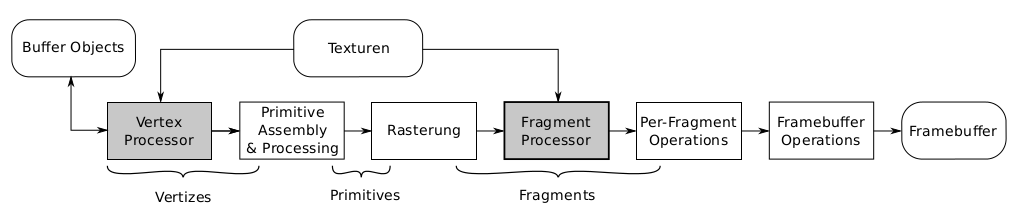
\includegraphics[width=15cm]{images/graphics_pipeline}
\caption{Die OpenGL-Grafikpipeline. Programmierbare Schnittstellen sind hervorgehoben.}
\label{fig:opengl_graphics_pipeline}
\end{figure}

Wie in OpenCL gibt es grundsätzlich zwei Datenstrukturen, die in
OpenGL als Eingabe fungieren können: Buffer und Texturen. Buffer
werden im Allgemeinen zur Speicherung geometrischer Daten verwendet,
\Pimiddydh{} Arrays von Vertizes und Primitiven. Texturen gleichen image
objects in OpenCL\@. Es sind mehrdimensionale Datenstrukturen mit
speziell definierten Attributen und Operationen, die \PimiddyzB{}
verschiedene Arten von Interpolation erlauben. Sie können ein-, zwei-
oder dreidimensionale Bilddaten repräsentieren.

Die zu verarbeitenden Objekte liegen als Vertizes in einer definierten
Reihenfolge in Form von Vertex- und Indexbuffern vor. Beim Zeichnen
gibt man eine Topologie für diese Vertizes an. In dieser Arbeit werden
Punkte (Point Sprites) und Dreiecke als Topologien
verwendet. Dreiecksnetze nennt man auch \PimiddyBegriff{Meshes}. Sie
werden \PimiddyzB{} aus einer Modeldatei geladen oder algorithmisch
erstellt (siehe \cref{sec:fallen_snow}).

Die einzelnen Vertizes werden über einen \PimiddyBegriff{Vertex Shader}
verarbeitet, der als Ausgabe Vertexattribute setzt oder modifiziert,
wie etwa Position, Texturkoordinaten und Normalen. Die transformierten
Vertizes werden dann über fest eingebaute, \Pimiddydh{} nicht
programmierbare, Verarbeitungsschritte zu Grafikprimitiven
zusammengesetzt und gerastert.

Dabei wird bestimmt, welche Teile der Geometrie sichtbar sind und
welche Primitive welche Bereiche des Bildes (\PimiddyzB{} Framebuffer)
überdecken. Das Ergebnis der Rasterung sind Fragments, die im
\PimiddyBegriff{Fragment Shader} manipuliert werden können. Ein
Fragment ist eine Datenstruktur, welche die zu einem einzelnen Pixel
gehörigen Daten eines Primitivs enthält. Mehrere Fragments können zu
einem Pixel gehören, etwa bei überlappender Geometrie, aber ein
Fragment beeinflusst immer nur höchstens ein Pixel des fertigen
Bildes.

Jedes Fragment besteht aus festen Datenfeldern, wie Tiefeninformation
und Bildschirmkoordinaten. Zusätzlich kann das Shaderprogramm
beliebige weitere vertexbezogene Daten vom Vertexshader übergeben
bekommen. Die Transformierung von Vertexdaten in Fragmentdaten
geschieht im Rasterungsschritt durch Interpolation. Die Ausgabe eines
Fragmentshaders besteht aus Farb- und Tiefeninformation, die am Ende
der Pipeline in eine spezielle Datenstruktur, den sogenannten
Framebuffer, geschrieben werden. Im einfachsten Fall ist dies der
Puffer, der das am Bildschirm dargestellte Bild im Speicher der
Grafikkarte repräsentiert. Es sind aber über sogenannte Framebuffer
Objects auch andere benutzerdefinierte Ausgaben möglich, die
geschrieben und \PimiddyzB{} als Texturen in weiteren Renderdurchgängen
durch die Pipeline wiederum als Input für andere Shader verwendet
werden können.  Die in dieser Arbeit verwendeten Shader sind in der
OpenGL Shading Language (GLSL) geschrieben, einer höheren
Programmiersprache mit C-ähnlicher Syntax, die zur Ausführung auf der
Grafikkarte mit OpenGL zu binärem Shadercode kompiliert wird.

Alle Versionen von GLSL unterstützen if-else-Verzweigungskonstrukte
wie in C und Schleifen.  Hardware mit voller Unterstützung für OpenGL
2.0, mit der Einführung von GLSL, wurde um 2003--2004 sowohl von NVidia
als auch von ATI auf den Markt gebracht.

\section{Windsimulation}
\label{sec:implementation_wind}

\subsection{Einleitung}

In diesem Abschnitt wird die Umsetzung der Windsimulation
vorgestellt. Da dieser Teil der Implementierung nicht mit der
Darstellung zusammenhängt, wird nur OpenCL verwendet. Der Abschnitt
knüpft direkt an \autoref{sec:stam} an.

Zuerst wird die Wahl der Datenstrukturen besprochen. Es kommt hier
darauf an, eine möglichst performante Struktur zu wählen, die optimale
Zugriffszeiten liefert. Danach wird das Verfahren von Stam in
OpenCL-Code übertragen, dessen Bestandteile detailliert erläutert
werden.

Schließlich wird besprochen, wie die Hindernisse in die
Simulation eingespeist werden.

\subsection{Allgemeines}

Für die Simulation des Winds ist es wichtig, eine möglichst optimale
Datenstruktur zur Speicherung der verwendeten Felder zu verwenden, um
die Speicherzugriffszeiten zu minimieren und die maximale Performance zu
erreichen.

Wie bereits angesprochen bietet OpenCL zur Speicherung die Wahl
zwischen buffer objects und image objects (sofern image objects auf der
Zielplattform unterstützt werden). Beide Speicherarten haben leicht
unterschiedliche Anwendungsgebiete, daher müssen erst die
Anforderungen erarbeitet werden, die man an die Datenstruktur
stellt.

In vielen Kerneln ist man daran interessiert, den Wert für die
\PimiddyQuotes{aktuelle} Zelle im Gitter sowie den Wert aller
Nachbarzellen zu bestimmen. Der \PimiddyQuotes{Wert} kann je nach
betrachtetem Feldtyp entweder Druck, Geschwindigkeit oder etwas
anderes bedeuten. Bei der Advektion wird außerdem linear zwischen den
Voxeln in einer Nachbarschaft linear \emph{interpoliert}.

\begin{figure}[h]
\centering
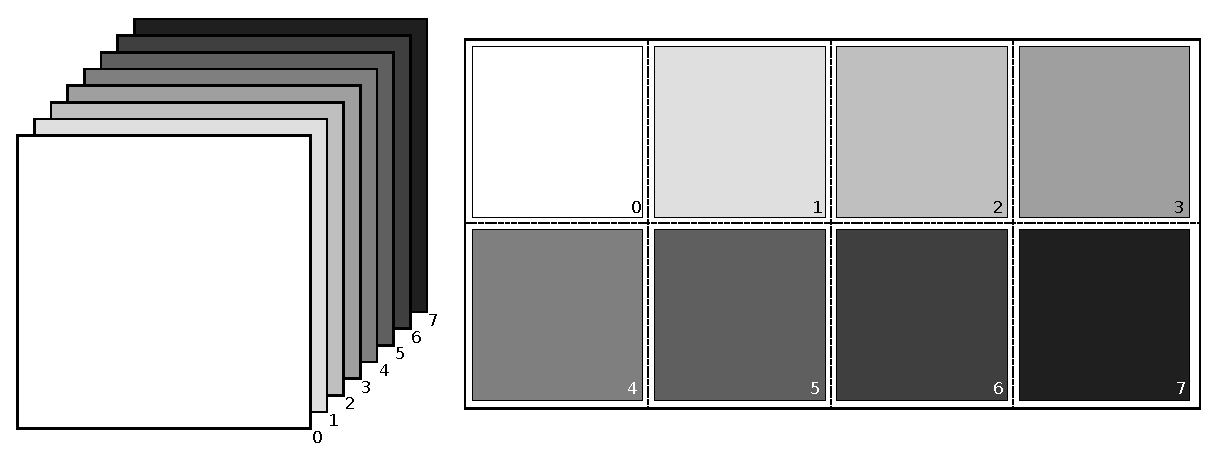
\includegraphics[width=14cm]{images/flat_texture}
\caption{Veranschaulichung einer Flat-3D-Textur}
\label{fig:implementation_flat_3d_texture}
\end{figure}

Schnelle Zugriffe auf einen Voxel samt seiner Nachbarn sind ein
Performancemerkmal von image objects. Sie würden sich daher für viele Kernel
anbieten, und viele GPU-Implementierungen von
strömungsmechanischen Verfahren nutzen in der Tat image objects (wenn auch
oft aus historischen Gründen). Allerdings ist das Schreiben von
3D-Texturen in OpenCL-1.1 nur mit einer Extension möglich. Als
Hilfsmaßnahme greift man hier üblicherweise zu sogenannten
\PimiddyBegriff{Flat-3D-Texturen} \cite{Harris2003}. Hier werden die
einzelnen \PimiddyQuotes{Scheiben} der dreidimensionalen Struktur
nebeneinander in eine zweidimensionale Textur geschrieben, siehe
\autoref{fig:implementation_flat_3d_texture}. Für die Umrechnung
zwischen 3D- und 2D-Koordinaten ist etwas Rechenaufwand
nötig. 2D-Texturen erlauben außerdem natürlicherweise nur
zweidimensionale Interpolation zwischen den Zellen. Benötigt man
hingegen dreidimensionale Interpolation, ist auch hier etwas
Mehraufwand zu verrechnen.

Image objects werden in einer optimierten Weise gespeichert, sodass
Leseoperationen beschleunigt werden. Diese optimierte Speicherung
führt aber dazu, dass das Schreiben in Texturen relativ langsam
ist. Selbst durchgeführte Benchmarks\PimiddyTodo{diese noch ergänzen?
Dazu einfach das Jacobiverfahren mit Texturen umsetzen und direkt
vergleichen (alles in 2D)} zeigen, dass buffer objects sogar im
Zweidimensionalen schneller sind als image objects. Daher wurden image objects
als mögliche Speicherform verworfen und es wurden einzig Buffer
verwendet. Diese erweisen sich außerdem als kompatibler, denn
OpenCL-Implementierungen müssen image objects nicht unterstützen.

Da Buffer eindimensional sind, muss zwischen drei- und
eindimensionalen Koordinaten konvertiert werden. Sei $(x,y,z)$ eine
dreidimensionale Koordinate und seien $(w,h,d)$ die Dimensionen eines
Buffers (er enthält also $w \cdot h \cdot d$ Elemente). Dann erhält
man einen eindimensionalen Index $i$ mittels:
\begin{equation}
\label{eq:implementation_wind_3d_to_2d}
i = w \cdot h \cdot z + w \cdot y + x
\end{equation}
Umgekehrt erhält man die $(x,y,z)$-Koordinaten eines Index mittels
\begin{equation}
\begin{split}
x &= i \PimiddyModulo w \\
y &= (i / w) \PimiddyModulo h \\
z &= i / (w \cdot h)  \\
\end{split}
\end{equation}
Im Folgenden wird das Verfahren von Stam in OpenCL umgesetzt. Fast
alle Kernel greifen hierbei auf den Buffer zurück, der die
Hindernisinformationen enthält. Im letzten Abschnitt wird erklärt, wie
dieser Buffer gefüllt wird.

\subsection{Verfahren nach Stam in OpenCL}

\subsubsection{Allgemeines}
\label{sec:implementation_wind_stam_general}

Es sollen nun die einzelnen Schritte des Verfahrens in OpenCL-Kernel
umgewandelt werden. Der Teil des Programms, der auf dem Host läuft,
soll hier nicht in Gänze erarbeitet werden. Stattdessen soll deutlich
werden, in welcher Reihenfolge die Kernel aufgerufen werden und welche
Daten beim Aufruf gelesen und geschrieben werden. Aus
Einrückungsgründen werden einige Bezeichner abgekürzt, aber immer so,
dass aus der Erläuterung \Pimiddybzw den Kommentaren noch hervorgeht, was
sich dahinter verbirgt.

Die Simulation benötigt einige persistente Daten, also solche, die
zwischen den Simulationsschritten beibehalten werden und nicht nur
temporär für Berechnungen verwendet werden:

\begin{itemize}
\item ein Buffer \PimiddyInlineCode{boundaries} vom Typ
\PimiddyInlineCode{float}, der 1.0 enthält, wenn die zugehörige
Gitterzelle ein Hindernis enthält und 0.0 wenn nicht. Das Befüllen
dieses Buffers wird in
\autoref{sec:implementation_wind_boundaries} beschrieben.
\item ein Buffer \PimiddyInlineCode{velocity} vom Typ
\PimiddyInlineCode{float3}, der das aktuelle Geschwindigkeitsfeld enthält.
Dieses Feld wird anfangs auf $(0,0,0)$ gesetzt. Der Wind wird manuell von
einer Seite in die Simulation gespeist (siehe
\autoref{sec:implementaion_wind_in_outflow}) und breitet sich dann
aus.
\item Viele der Algorithmen benötigen außerdem das aktuelle
\PimiddyQuotes{Zeitdelta} \PimiddyInlineCode{float dt}. Es gibt die
Zeit an, die seit dem letzten Simulationsdurchlauf vergangen ist. Mit
Hilfe dieser Größe wird die Simulation zeitlich normiert. Lange
Zeitabstände zwischen den diskreten Frames sollen zu größeren
Veränderungen im Windfeld führen.
\end{itemize}

Die meisten Kernel werden mit einer dreidimensionalen Arbeitsgröße
initialisiert, die der Größe des Gitters entspricht. Ein Work-Item
erhält also einen dreidimensionalen Vektor als globale ID, welcher die
Gitterposition angibt, die das Work-Item bearbeiten soll.

Da die buffer objects mit den Feldern allerdings eindimensional sind,
bietet es sich an, den Übergang von einem drei- zu einem
eindimensionalen Index in eine Funktion auszulagern. Diese Funktion
kann gleichzeitig testen, ob die gegebene Position den Rand des
Gitters verlässt, und in dem Fall den nächstgelegenen Voxel am Rand
zurückliefern. So lassen sich auf einfache Weise alle Nachbarn eines
Voxels aus dem Buffer extrahieren.

Die Funktion \PimiddyInlineCode{i4p} ist im Folgenden
dargestellt\PimiddyTodo{Das \PimiddyInlineCode{uint} wird nicht
highlighted}:

\begin{minted}[frame=lines,mathescape]{opencl}
// Bekommt die Gittergroesse s und eine 3D-Position p.
// Liefert einen Index.
uint i4p(uint3 p,uint3 s)
{
    // Komponentenweise in gueltigen
    // Bereich $[0,n-1]$ transformieren
    p = clamp(
        p,
        (uint3)(0),
        s - 1);

    return s.w * s.h * p.z + s.w * p.y + p.x;
}
\end{minted}

Für die Indextransformation wurde
\autoref{eq:implementation_wind_3d_to_2d} verwendet.  Die
Standardbibliotheksfunktion \PimiddyInlineCode{clamp} stellt sicher,
dass ein Wert innerhalb eines Intervalls bleibt:
\begin{align}
\PimiddyFormelText{clamp}(x,a,b) = \max \{ a,\min \{ b,x \} \}
\end{align}

\subsubsection{Advektion}
\label{sec:implementation_wind_advection}

\begin{figure}
	\begin{subfigure}[t]{0.5\textwidth}
		\centering
		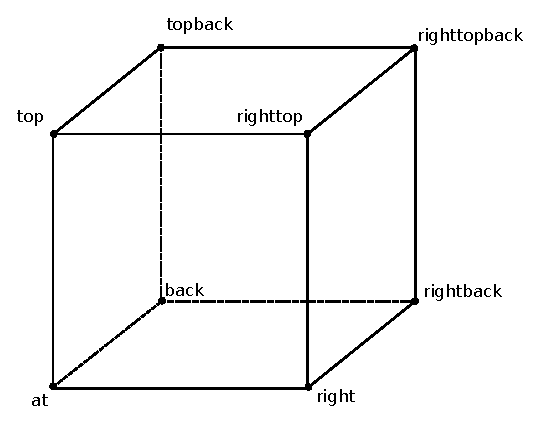
\includegraphics[width=\textwidth]{images/right_neighborhood}
                \caption{Veranschaulichung der Nachbarschaftsstruktur \PimiddyInlineCode{neighbors}.}
                \label{fig:implementation_right_neighbors}
	\end{subfigure}
	~
	\begin{subfigure}[t]{0.5\textwidth}
		\centering
		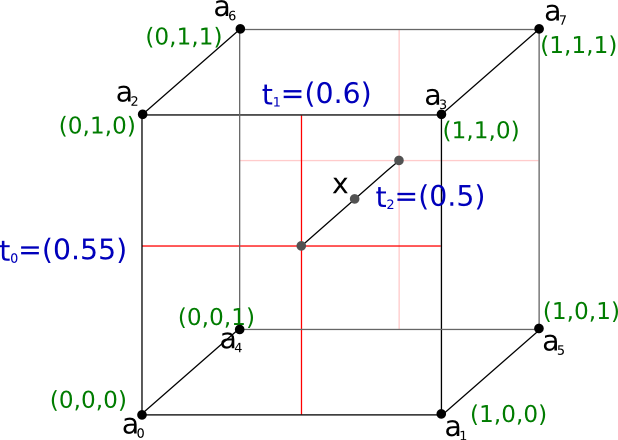
\includegraphics[width=\textwidth]{images/ndinterpolation}
		\caption{Dreidimensionale Interpolation mit dem Beispielvektor $(0.55,0.6,0.0.5)$}
		\label{fig:implementation_wind_interpolation}
	\end{subfigure}
	\caption{Die dreidimensionale Nachbarschaft \PimiddyInlineCode{neighbors}}
\end{figure}

Der erste Schritt im Verfahren von Stam ist die Advektion des
Vektorfeldes \PimiddyInlineCode{velocity}
(\Pimiddyvgl \autoref{sec:stam_advection}). Der dazugehörige Kernel ist in
mehrere Funktionen und Strukturen aufgeteilt, die nun im einzelnen
erklärt werden.

Vom aktuellen Voxel aus verfolgt man den Geschwindigkeitspfeil in
\PimiddyInlineCode{velocity} zurück und landet dabei -- weil der
Geschwindigkeitspfeil eben ein \PimiddyInlineCode{float3} ist -- im
Allgemeinen zwischen 8 Gitterzellen. Diese 8 Zellen nutzt man für eine
lineare Interpolation, um die neue Geschwindigkeit zu finden. Es
bietet sich an, zunächst eine Struktur zu definieren, um einen
Geschwindigkeitswert sowie die direkten Nachbarn zu speichern (siehe
\autoref{fig:implementation_right_neighbors}).

\begin{minted}[frame=lines]{c}
typedef struct
{
    float3 at;
    float3 right,top,back,righttop;
    float3 rightback,topback;
    float3 righttopback;
} neighbors;
\end{minted}

Eine Instanz dieser Struktur wird von der zugehörigen Funktion
\PimiddyInlineCode{neighbors\_for\_pos} zurückgegeben, die eine
beliebige (diskrete) Position im Gitter sowie die Größe des Gitters
als Eingabe erhält. Die Funktion greift auf \PimiddyInlineCode{i4p}
zurück und ist so gegen Zugriffe außerhalb des Gitters geschützt:

\begin{minted}[frame=lines]{c}
// Parameter genau wie i4p, zusaetzlich noch "b"
neighbors neighbors_for_pos(
    global float3 *b,
    uint3 p,
    uint3 s)
{
    neighbors result;
    result.at = b[i4p(p,s)];
    result.right = b[i4p(p+(uint3)(1,0,0),s)];
    result.top = b[i4p(p+(uint3)(0,1,0),s)];
    result.back = b[i4p(p+(uint3)(0,0,1),s)];
    result.righttop = b[i4p(p+(uint3)(0,1,1),s)];
    result.rightback = b[i4p(p+(uint3)(1,0,1),s)];
    result.topback = b[i4p(p+(uint3)(0,1,1),s)];
    result.righttopback = b[i4p(p+(uint3)(1,1,1),s)];
    return result;
}
\end{minted}

Mit Hilfe einer Instanz von \PimiddyInlineCode{neighbors} und einem
beliebigen Vektor im Einheitsintervall $[0,1]^3$ soll ein
interpolierter Vektor erzeugt werden. Hier hilft die OpenCL-C-Funktion
\PimiddyInlineCode{mix}, die linear zwischen zwei Werten anhand eines
dritten Wertes interpoliert:
\begin{align}
\PimiddyFormelText{mix}(a,b,x) = (1-x)\cdot a + x \cdot b
\end{align}
Diese Funktion wird speziell auf Grafikkarten in hocheffektiven Code
übersetzt, da sie sich auf sogenannte
\PimiddyQuotes{multiply-add-Operationen} (auch
\PimiddyQuotes{MAD} genannt) zurückführen lässt. Darunter versteht man
skalare Operationen der Form $a\cdot x + b$, also eine Multiplikation
gefolgt von einer Addition. Da dies in der Grafikpipeline häufig
auftritt, sind die Arithmetikchips einer GPU speziell darauf
ausgelegt. Auf \PimiddyInlineCode{mix} wird in der unten stehenden
\PimiddyInlineCode{interpolate\_neighbors} mehrfach zurückgegriffen:

\begin{minted}[frame=lines,mathescape]{c}
float3 interpolate_neighbors(
    neighbors n,
    // v ist ein Vektor im Intervall $[0,1]^3$
    float3 v)
{
    float3
        v1 = mix(
            mix(n.at, n.right, v.x),
            mix (n.top, n.righttop, v.x),
            v.y),
        v2 = mix(
            mix(n.back, n.rightback, v.x),
            mix(n.topback, n. righttopback, v.x),
            v.y);

    return mix(v1,v2,v.z);
}
\end{minted}

Das Funktionsprinzip ist am Beispiel in
\autoref{fig:implementation_wind_interpolation} verdeutlicht. Es wird
erst vier mal auf der $x$-Achse interpoliert, dann zwei mal auf der
$y$-Achse und schließlich einmal auf der $z$-Achse.

Der eigentliche Advektionskernel hat schließlich folgende Form:

\begin{minted}[frame=lines]{c}
kernel void advection(
    global float *boundary,
    global float3 *input,
    global float3 *output,
    // Das Zeitdelta
    float dt,
    // Gibt die Gittergroesse an
    uint3 size)
{
    uint3 position = (int3)(
        get_global_id(0),
        get_global_id(1),
        get_global_id(2));

    uint index = i4p(position,size);

    if(boundary[index] != 0.0f)
    {
        output[index] = (float3)(0.0f);
        return;
    }

    float3
        v = input[index],
        // Konvertiere mit convert_float3 die diskrete Position
        // in eine Fliesskommaposition. Fuehre dann Advektion durch.
        advected = convert_float3(position) - dt * v,
        // fract liefert den Fliesskommateil eines Vektors.
        fractions = fract(advected_vector);

    neighbors n = neighbors_for_pos(
        input,
        position,
        size);

    output[index] = interpolate_neighbors(
        n,
        fractions);
}
\end{minted}

\subsubsection{In- und Outflow}
\label{sec:implementaion_wind_in_outflow}

Nach der Advektion werden die In- und Outflowboundaries behandelt
(\Pimiddyvgl \autoref{sec:stam_boundaries}). Im Gegensatz zu den anderen
Kerneln wird hier nicht das gesamte Feld als globale Arbeitsgröße
gewählt, sondern nur eine Teilmenge des Gitters. Die Kernel sind so
einfach gehalten, dass sie hier nur erläutert, aber nicht im Code
vorgestellt werden.

Die Inflow-Boundaries gestalten sich sehr einfach. Es wird ein Vektor
vorgegeben, der die momentane Windstärke und -richtung angibt. Dann
wird eine Seite des Simulationswürfels mit diesem Vektor
gefüllt. Stams Verfahren sorgt dafür, dass sich der Wind langsam im
Simulationsbereich ausbreitet.

Bei den Outflow-Boundaries werden die 6 Randseiten des Würfels separat
behandelt. Jede Seite wird in die jeweils benachbarte
\PimiddyQuotes{Scheibe} kopiert; für die linke Seite in die Scheibe
rechts daneben, die Oberseite in die Scheibe einen drunter, und so
weiter\PimiddyTodo{Hier noch ein Bild von?}.

\subsubsection{Projektion}
\label{sec:implementation_wind_projection}

\begin{figure}[ht]
\centering
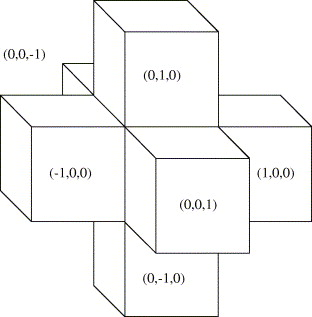
\includegraphics[width=6cm]{images/von_neumann}
\caption{Die dreidimensionale Von Neumann-Nachbarschaft}
\label{fig:implementation_wind_von_neumann_neighbors}
\end{figure}

Nach der Advektion ist das Vektorfeld $\vec{u}$ nicht mehr quellenfrei
und der Projektionsoperator muss angewendet werden
(\Pimiddyvgl \autoref{sec:stam_projection}). Dazu bestimmt man zuerst die
Divergenz $\PimiddyDiv \vec{u}$ des Vektorfeldes und löst dann das
Gleichungssystem $\PimiddyLaplace x = \PimiddyDiv \vec{u}$ nach $x$
mit Hilfe des Jacobiverfahrens. Der Gradient von $x$ wird schließlich
von $\vec{u}$ subtrahiert und das Feld ist wieder quellenfrei.

Man benötigt also zunächst die Divergenz des Vektorfeldes. Analog zur
Advektion wird eine Struktur definiert, um die Von
Neumann-Nachbarschaft eines Gitterpunktes zu speichern (siehe
\autoref{fig:implementation_wind_von_neumann_neighbors}):

\begin{minted}[frame=lines]{c}
typedef struct vn_neighbors
{
    float3 at;
    float3 left, right;
    float3 top, bottom;
    float3 front, back;
    float boundary_at;
    float boundary_left, boundary_right;
    float boundary_top, boundary_bottom;
    float boundary_front, boundary_back;
};
\end{minted}

Die Struktur enthält zusätzlich die zu den Nachbarn gehörigen
Hinderniswerte. Die Bestimmung dieser Werte und die der Vektoren
verläuft nach demselben Schema wie bei der Advektion und sei im
Folgenden ohne den zugehörigen Code mit
\PimiddyInlineCode{vn\_neighbors\_for\_pos(...)}  bezeichnet.

Bei der Bestimmung der Divergenz müssen die Randbedingungen beachtet
werden. Ist einer der Nachbarn des aktuellen Voxels von einem
Hindernis ausgefüllt, wird statt des Vektors an dieser Stelle der
\emph{Nullvektor} angenommen:
\begin{minted}[frame=lines]{c}
vn_neighbors n = vn_neighbors_for_pos(...);
if(n.boundary_left != 0.0f)
    n.left = (float3)(0.0f);
\end{minted}
Statt dies jedoch als eine \PimiddyInlineCode{if}-Bedingung
umzusetzen, wird stattdessen eine Multiplikation mit dem Randwert
verwendet.

Dies rührt daher, dass GPUs sich suboptimal verhalten, wenn mehrere
Work-Units in einer Work-Group unterschiedliche Ausführungspfade durch
den Code nehmen. Bei einer \PimiddyInlineCode{if}-Abfrage, die
beispielsweise für nur ein Work-Item \PimiddyInlineCode{true} ergibt,
durchlaufen dennoch \emph{alle} Work-Units der Work-Group den Rumpf
des \PimiddyInlineCode{if}-Statements, wobei die Ergebnisse der
\PimiddyQuotes{toten} Ausführungspfade verworfen werden. Natürlich
geschieht dies transparent für den Anwender, sodass keine
unerwünschten Nebeneffekte eintreten.

Die obige Abfrage lässt sich wie folgt umschreiben:

\begin{minted}[frame=lines]{c}
vn_neighbors n = vn_neighbors_for_pos(...);
n.left = (1.0f - n.boundary_left) * n.left;
\end{minted}

Hier liegt wieder eine MAD-Operation vor, der Code ist also wieder
sehr effizient.

Der zur Divergenz gehörige Kernel hat die folgende Form:

\begin{minted}[frame=lines]{c}
kernel void divergence(
    global float3 *input,
    global float *output,
    global float *boundary,
    uint3 size)
{
    uint4 position = (int3)(
        get_global_id(0),
        get_global_id(1),
        get_global_id(2));

    uint index = i4p(position,size);

    vn_neighbors n = vn_neighbors_for_pos(
        input,
        position,
        boundary,
        size);

    float3 z = (float3)(0.0f);

    // Hier geschieht die Behandlung der Randbedingungen.
    // Es wird ausgenutzt, dass die Randwerte die Werte 0 oder 1
    // annehmen.
    n.left = mix(n.left, z, n.boundary_left);
    n.right = mix(n.right, z, n.boundary_right);
    n.top = mix(n.top, z, n.boundary_top);
    n.bottom = mix(n.bottom, z, n.boundary_bottom);
    n.front = mix(n.front, z, n.boundary_front);
    n.back = mix(n.back, z, n.boundary_back);

    // Da die Gittergroesse 1 betraegt, vereinfacht sich die Formel
    // aus dem ersten Abschnitt ein wenig.
    output[index] =
        (n.right - n.left).x +
        (n.bottom - n.top).y +
        (n.front - n.back).z;
}
\end{minted}

Um die Ähnlichkeit mit den restlichen Kerneln aufzuzeigen wurde hier
wieder die Funktion \PimiddyInlineCode{mix} verwendet.

Anschließend wird das Jacobiverfahren durchgeführt. Das
Verfahren ist iterativ, der Jacobi-Kernel muss also mehrfach gestartet
werden. Um Speicherplatz zu sparen, bietet sich ein
\PimiddyQuotes{Ping-Pong-Schema} an. Dazu werden zwei zusätzliche
buffer objects \PimiddyInlineCode{s1,s2} benötigt, welche jeweils ein
Skalarfeld speichern. Anfangs enthält \PimiddyInlineCode{s1} die
initiale Lösung für die Poissongleichung $\PimiddyLaplace x =
\PimiddyDiv \vec{u}$, also einfach das Nullfeld $x=0$. Eine Anwendung des
Jacobi-Kernels füllt \PimiddyInlineCode{s2} mit der ersten Iteration
des Verfahrens. Diese wird zur Eingabe der nächsten Iteration, die
\PimiddyInlineCode{s1} überschreibt, und so weiter. Nach gerade vielen
Iterationsschritten enthält \PimiddyInlineCode{s1} die endgültige
Lösung. \autoref{alg:implementation_wind_ping_ping} zeigt das
Verfahren im Pseudocode.

\begin{algorithm}
\caption{Der Ping-Pong-Algorithmus für das Jacobiverfahren}
\label{alg:implementation_wind_ping_ping}
\begin{algorithmic}
\Function{jacobi}{$\PimiddyDiv u$,b}
	\State s1 $\gets$ clCreateBuffer
	\State s2 $\gets$ clCreateBuffer
        \State fill\_buffer(s1,0)
        \State current\_source $\gets$ s1
        \State current\_destination $\gets$ s2
        \State clSetKernelArg(jacobi,0,$\PimiddyDiv u$)
        \State clSetKernelArg(jacobi,1,b)
        \For{i = 0; i < iterations; i++}
            \State clSetKernelArg(jacobi,2,current\_source)
            \State clSetKernelArg(jacobi,3,current\_destination)
            \State clEnqueueNDRangeKernel(jacobi)
            \State swap(current\_source,current\_destination)
        \EndFor
        \State \Return s1
\EndFunction
\end{algorithmic}
\end{algorithm}

Die Randbedingungen im Jacobi-Kernel werden ähnlich denen im
Divergenz-Kernel behandelt. Ist einer der Nachbarn von einem Hindernis
ausgefüllt, wird statt des Vektors an dieser Stelle der Vektor im
\emph{Zentrum der Nachbarschaft} angenommen. Dies lässt sich auch mit
der Operation \PimiddyInlineCode{mix} durchführen.

\begin{minted}[frame=lines]{c}
kernel void jacobi(
    global float *divergence,
    global float *boundary,
    global float3 *input,
    global float *output,
    uint3 size)
{
    uint4 position = (int3)(
        get_global_id(0),
        get_global_id(1),
        get_global_id(2));

    uint index = i4p(position,size);

    vn_neighbors n = vn_neighbors_for_pos(
        input,
        position,
        boundary,
        size);

    n.left = mix(n.left, n.at, n.boundary_left);
    n.right = mix(n.right, n.at, n.boundary_right);
    n.top = mix(n.top, n.at, n.boundary_top);
    n.bottom = mix(n.bottom, n.at, n.boundary_bottom);
    n.front = mix(n.front, n.at, n.boundary_front);
    n.back = mix(n.back, n.at, n.boundary_back);

    float sum    = n.left + n.right + n.top + n.bottom + n.front + n.back,
          result = (sum - divergence[index]) / 6.0f;

    output[index] = mix(
        result,
        center,
        1.0f/3.0f);
}

\end{minted}

Der Code zeigt die gewichtete Jacobi-Iteration mit Wichtungswert
$\frac{1}{3}$, der sich als günstig herausgestellt hat.

Die Zahl der Iterationen kann von der Leistung der Grafikkarte
abhängig gemacht werden. Sie sollte jedoch mindestens 20
betragen. Gute Ergebnisse werden bei 40 Iterationen
erzielt. \autoref{fig:implementation_wind_jacobi_times} zeigt die
Laufzeit für verschiedene Iterationszahlen.

\begin{figure}[ht]
\centering
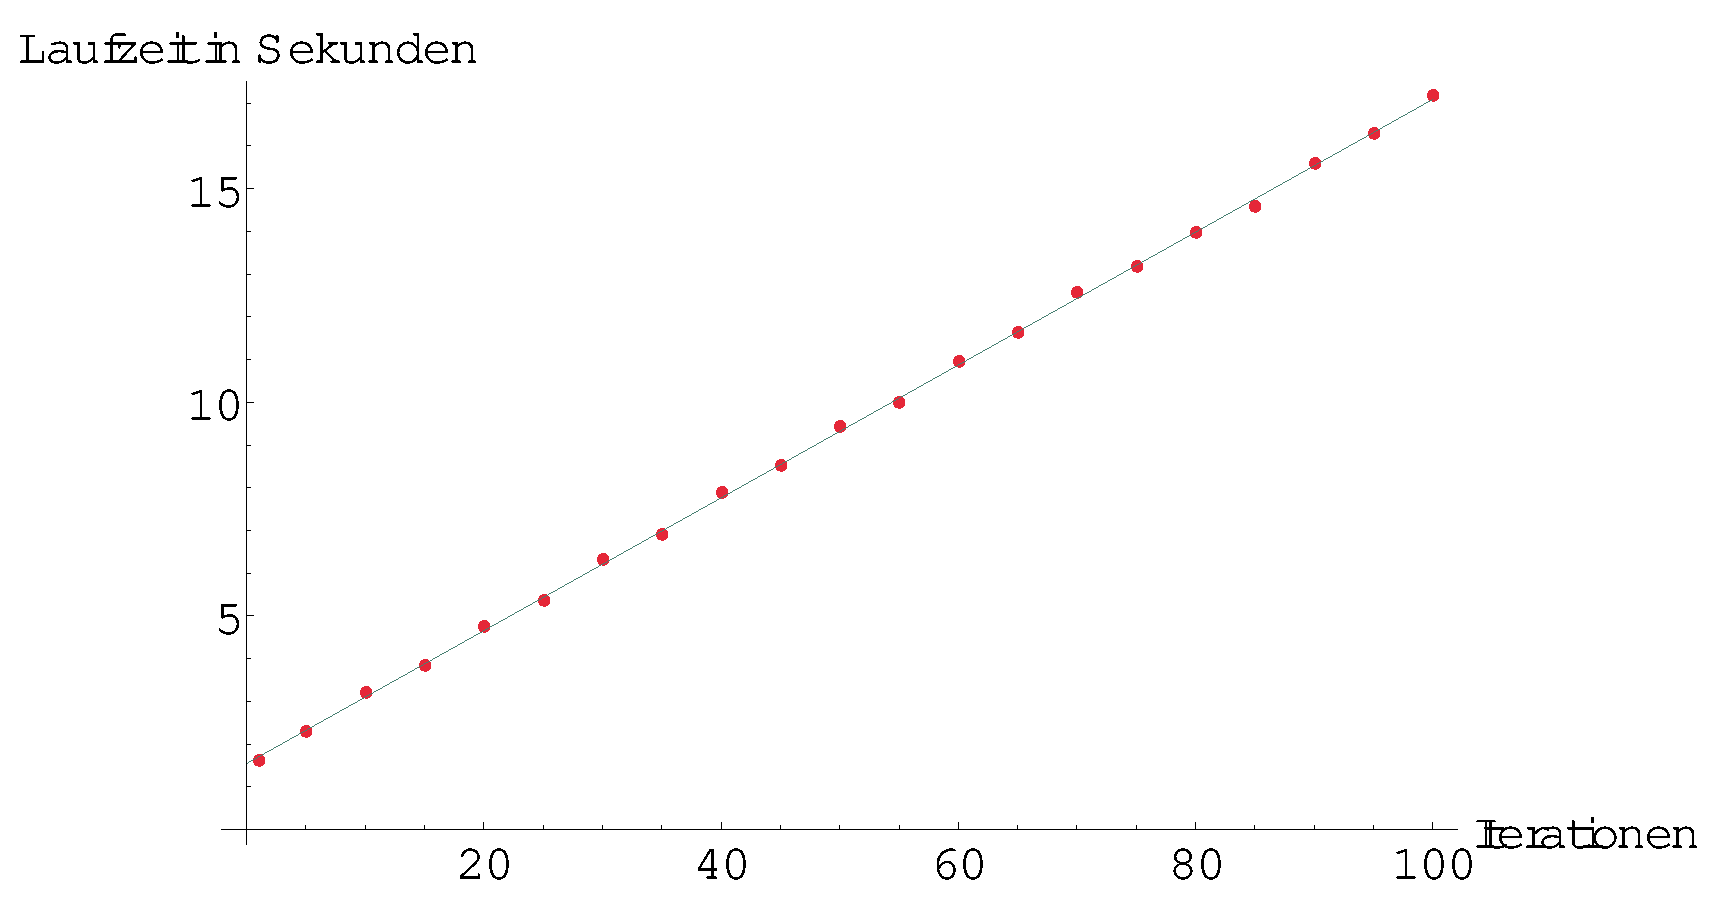
\includegraphics[width=13cm]{images/jacobi_times}
\caption{Die Laufzeit für verschiedene Jacobi-Iterationszahlen. Es ergibt sich ein linearer Zusammenhang. Die entsprechende Ausgleichsgerade ist ebenfalls eingezeichnet.}
\label{fig:implementation_wind_jacobi_times}
\end{figure}

Die Berechnung des Gradienten von $x$ und die darauf folgende
Subtraktion von $\vec{u}$ lässt sich (auch aus Performancegründen) in
einem einzigen Kernel behandeln. In diesem Kernel werden auch die vom
Jacobi-Verfahren nur unvollständig gelösten Randbedingungen
erzwungen. Der Kernel erfüllt folgende Aufgaben:

\begin{enumerate}
\item Er bestimmt den Gradienten des Druckfeldes. Es wird für einen
Nachbarwert wieder der Wert im Zentrum genommen, falls die
Nachbarzelle von einem Hindernis ausgefüllt ist.
\item Der Gradient wird vom Geschwindigkeitsfeld abgezogen.
\item Die free-slip-Randbedingungen werden erzwungen.
\end{enumerate}

\begin{figure}[h]
\centering
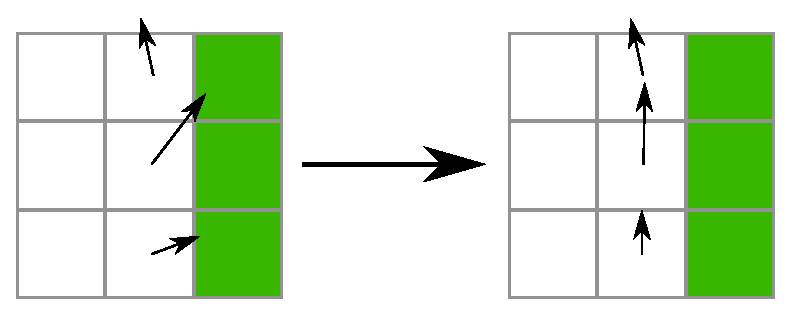
\includegraphics[width=10cm]{images/force_free_slip}
\caption{Die Korrektur der nach dem Projektionsschritt eventuell noch unvollständig gelösten Randbedingungen. Die markierten Felder enthalten Hindernisse, die $x$-Komponente der Geschwindigkeit wird daher auf $0$ gesetzt.}
\label{fig:implementation_wind_enforce_free_slip}
\end{figure}

In Schritt 3 wird für jede Koordinatenachse gespeichert, ob sich in
der Von Neumann-Nachbarschaft auf der Achse ein Hindernis
befindet. Ist dies der Fall, wird die Geschwindigkeitskomponente auf
dieser Achse auf 0
gesetzt. \autoref{fig:implementation_wind_enforce_free_slip}
verdeutlicht das Prinzip. Der Koeffizient, der die entsprechende
Komponente entweder behält oder gleich 0 setzt, kann als Funktion der
beiden Randwerte auf der Achse ausgedrückt werden:
\begin{minted}[frame=lines]{c}
float boundary_mask(float boundary_left,float boundary_right)
{
  return 1.0f - min(1.0f, boundary_left + boundary_right);
}
\end{minted}
Offenbar ist die Funktion genau dann $0$, wenn einer der beiden Werte
0 ist. Die Funktion enthält zudem keine (expliziten) bedingten
Anweisungen. Der gesamte Kernel ergibt sich wie folgt:
\begin{minted}[frame=lines]{c}
kernel void subtract_pressure_gradient(
    global float3 *velocity,
    global float *boundary,
    global float *pressure,
    uint3 size)
{
    // Schritt 1: Bestimmte Gradient des Druckfeldes
    uint4 position = (int3)(
        get_global_id(0),
        get_global_id(1),
        get_global_id(2));

    uint index = i4p(position,size);

    vn_neighbors n = vn_neighbors_for_pos(
        input,
        position,
        boundary,
        size);

    if(boundary[index] == 1.0f)
    {
        velocity[current_index] =
            (float3)(
                0.0f,
                0.0f,
                0.0f);
        return;
    }

    float const center =
        pressure[index];

    // Bei Hinderniszellen wird das Zentrum gewaehlt
    n.left = mix(n.left, n.at, n.boundary_left);
    n.right = mix(n.right, n.at, n.boundary_right);
    n.top = mix(n.top, n.at, n.boundary_top);
    n.bottom = mix(n.bottom, n.at, n.boundary_bottom);
    n.front = mix(n.front, n.at, n.boundary_front);
    n.back = mix(n.back, n.at, n.boundary_back);

    float3 const pressure_gradient =
        (float3)(
            n.right.x - n.left.x,
            n.bottom.y - n.top.y,
            n.front.z - n.back.z);

    // Schritt 2 und 3: Gradient subtrahieren und Randbedingungen erzwingen
    float3 const vmask =
        (float3)(
            boundary_mask(n.boundary_left,n.boundary_right),
            boundary_mask(n.boundary_top,n.boundary_bottom),
            boundary_mask(n.boundary_front,n.boundary_back));

    velocity[current_index] =
        vmask * (velocity[index] - pressure_gradient);
}
\end{minted}

Das so erzeugte \PimiddyInlineCode{velocity}-Feld kann in der nächsten
Iteration wieder in die Advektionsroutine gegeben werden.

\subsection{Hindernisse in der Simulation}
\label{sec:implementation_wind_boundaries}

Bisher wurde das Hindernisfeld \PimiddyInlineCode{boundary} als
gegeben angenommen. Nun sollen Möglichkeiten vorgestellt werden, das
Feld mit Hinderniswerten zu füllen. Es wird zuerst ein Ansatz
beschrieben, bei dem Hindernisse aus primitiven Formen zusammengesetzt
werden. Danach werden Verfahren vorgestellt, um direkt aus einer
Meshdatei ein Hindernisfeld zu erzeugen.

\subsubsection{Einfacher Ansatz}

Oft ist die Geometrie von Hindernissen relativ einfach gestaltet, oder
sie wird speziell für die Simulation vereinfacht. Das angezeigte Mesh
hat dann gegebenenfalls wesentlich mehr Details als das diskretisierte
Hindernisfeld. Bewegen sich die Partikel schnell genug \Pimiddybzw
löscht man die Partikel erst eine gewisse Zeit nach der Kollision mit
den Hindernissen, ist der Detailunterschied nicht zu merken.

Es bietet sich daher an, die Hindernisse aus einfachen geometrischen
Formen wie Kugeln oder Quadern zusammenzusetzen. Diese Formen lassen
sich sehr einfach diskretisieren, was im folgenden besprochen werden soll.

Gegeben einer Menge von geometrischen Formen und einem Anfangs mit $0$
gefüllten Hindernisfeld, kann das endgültige Hindernisfeld
inkrementell konstruiert werden, indem immer weiter einzelne
Hindernisse hinzugefügt werden (sprich, Werte auf $1$ gesetzt
werden). Für jedes Primitiv benötigt man einen Kernel, der die
geometrischen Eigenschaften (\PimiddyzB Ausdehnung) sowie
\PimiddyInlineCode{boundary} erhält.

Für einen Quader $Q$, gegeben durch die drei Intervalle
$[x_1,x_2],[y_1,y_2],[z_1,z_2]$, ist dieser Kernel sehr einfach
gestaltet. Für jeden Voxel muss er testen, ob dessen Position
innerhalb des Quaders ist.

Für eine Kugel, gegeben durch einen Radius $r$ und eine Position
$(x,y,z)$ muss für jeden Voxel mit Position $(v_x,v_y,v_z)$ die
Kugelungleichung ausgewertet werden:

\begin{align}
(x-v_x)^2 + (y-v_y)^2 + (z-v_z)^2 \leq r^2
\end{align}

Ist sie wahr, wird der Voxel auf 1 gesetzt. Ähnlich einfach lässt sich
ein Ellipsoid behandeln, welcher durch drei Radien $r_x,r_y,r_z$ und eine
Position $(x,y,z)$ gegeben ist. Seine Ungleichung lautet:

\begin{align}
\frac{(x-v_x)^2}{r_x} + \frac{(y-v_y)^2}{r_y} + \frac{(z-v_z)^2}{r_z} \leq 1
\end{align}

Diese Art, Hindernisse einzubringen, ist allerdings sehr
zeitaufwändig, da stets zwei Modelle zu erstellen sind -- eins zur
Anzeige, bestehend aus einer Menge von Dreiecken, und eins für die
Simulation, bestehend aus geometrischen Formen. Die Konvertierung dieser
Formen zu Dreiecksnetzen ist zwar ohne Probleme möglich, es ist jedoch
ein sehr unnatürlicher Arbeitsablauf und es existieren keine Tools,
die dies vereinfachen könnten.

\subsubsection{Komplexe Hindernisse}

Es wäre günstiger, aus dem Mesh, was später angezeigt wird, das
Hindernisfeld zu gewinnen -- oder notfalls aus einem leicht
vereinfachten Mesh, welches rein visuell interessante Objekte nicht
enthält. Diesen Vorgang nennt man \PimiddyBegriff{Voxelization}. Im
Weiteren wird ein simpler Algorithmus vorgeschlagen, um diese Aufgabe
zu lösen. Für größere Felder ist dieser Algorithmus allerdings
ungeeignet, daher werden Alternativen besprochen.
\begin{figure}[h]
\centering
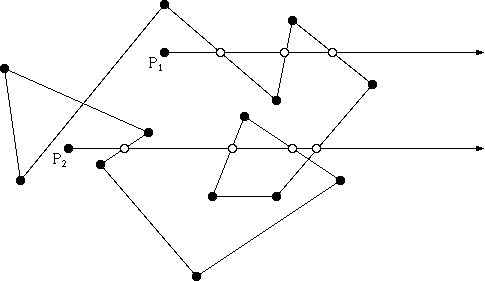
\includegraphics[width=10cm]{images/point_in_polygon}
\caption{Der einfache Test, ob ein Punkt in einem Körper enthalten ist, hier in zwei Dimensionen. $P_1$ hat 3 Schnittpunkte und ist innerhalb, $P_2$ hat 4 und ist somit außerhalb.}
\label{fig:implementation_wind_point_in_polygon}
\end{figure}
Gegeben sei eine Menge von Dreiecken, gegeben durch ihre Eckpunkte
(weitere Eigenschaften wie Normalen und Texturkoordinaten sind für die
Umwandlung nicht interessant). Die Menge von Dreiecken soll einen
geschlossenen Körper bilden, Löcher oder Überschneidungen sind nicht
erlaubt. Unter diesen Voraussetzungen lässt ich für jeden Gitterpunkt
in \PimiddyInlineCode{boundary} entscheiden, ob dieser innerhalb des
Körpers ist oder außerhalb: Man betrachtet eine Halbgerade vom
Gitterpunkt aus und zählt die Schnittpunkte der Geraden mit allen
Dreiecken des Körpers. Bei einer geraden Anzahl von Schnittpunkten ist
der Punkt außerhalb, sonst innerhalb (siehe
\autoref{fig:implementation_wind_point_in_polygon}).

Der Test ist arithmetisch sehr einfach gestaltet und
performant. Allerdings ist seine Laufzeit immernoch $O(n^3 \cdot k)$,
wobei $n$ die Größe des Gitters angibt und $k$ die Anzahl an
Dreiecken. Bei einem $64^3$ großen Feld und einem hinreichend
komplexen Modell mit $3.000$ Dreiecken kommt man bereits auf
786.432.000 Tests.

Die Implementierung eines effizienteren Verfahrens übersteigt den
Rahmen dieser Arbeit allerdings deutlich, daher wurde auf das Tool
\emph{binvox} zurückgegriffen\cite{binvox2012}. Es verwendet den
Algorithmus aus \cite{Nooruddin2003}, der auf \PimiddyQuotes{Ray
Stabbing} basiert, einer Abwandlung des eben beschriebenen
Verfahrens. Das Tool arbeitet parallel auf der GPU und liefert in
Sekunden Ergebnisse. Als Eingabe erhält es die Modeldatei im
obj-Dateiformat, welche vom Programm auch direkt zur Anzeige verwendet
wird. Die Ausgabe erfolgt in einem eigens geschrieben Dateiformat, dem
binvox-Format\cite{binvoxfileformat2012}. Eine
\PimiddyInlineCode{.binvox}-Datei hat den folgenden, einfachen Aufbau:

\begin{minted}{java}
#binvox 1
dim 128 128 128
translate -0.120158 -0.481158 -0.863158
scale 7.24632
data
...
\end{minted}

Die erste Zeile gibt die Version des Dateiformats an. Zum jetzigen
Zeitpunkt gibt es nur Version 1. Die nächste Zeile gibt die
Dimensionen des Gitters an. Die Werte für
\PimiddyInlineCode{translate} und \PimiddyInlineCode{scale} geben an,
wie das Gitter verschoben und skaliert werden muss, um mit dem
vorgegebene Model übereinzustimmen.

Danach folgen die eigentlichen Daten als rohe Bytes. Um Platz bei
großen Gittern zu sparen, sind sie \emph{lauflängenkodiert}. Das
Datensegment enthält eine Folge von Byte-Paaren. Das erste Byte in
einem Paar gibt an, ob eine Folge von Nullen oder Einsen folgt. Das
zweite Byte gibt an, wie viele Nullen oder Einsen folgen.

Die lineare Folge von Gitterpunkten wird mit der Festlegung zum
dreidimensionalen Gitter, dass sich die $y$-Koordinate am schnellsten
verändert, dann die $x$-Koordinate, dann die $z$-Koordinate.

\begin{figure}
	\begin{subfigure}[t]{0.5\textwidth}
		\centering
		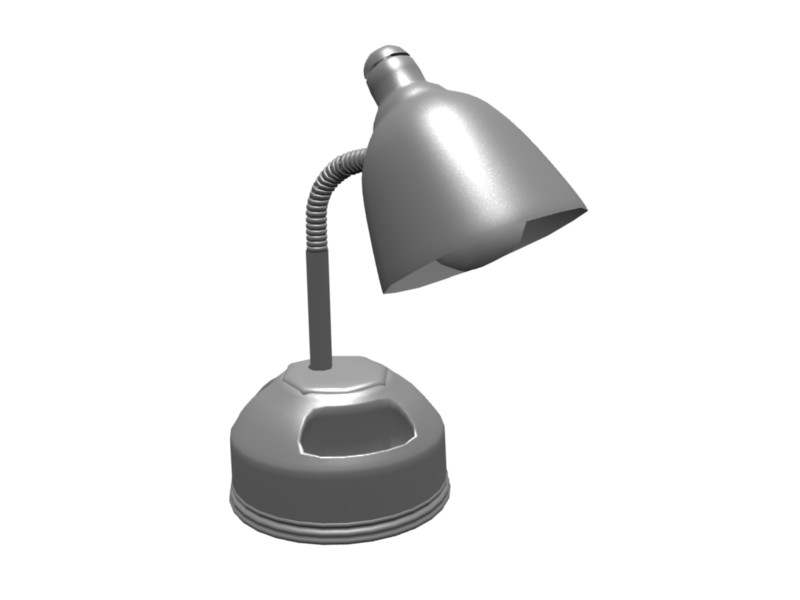
\includegraphics[width=\textwidth]{images/lamp_obj}
		\caption{Das Modell einer Lampe}
	\end{subfigure}
	~
	\begin{subfigure}[t]{0.5\textwidth}
		\centering
		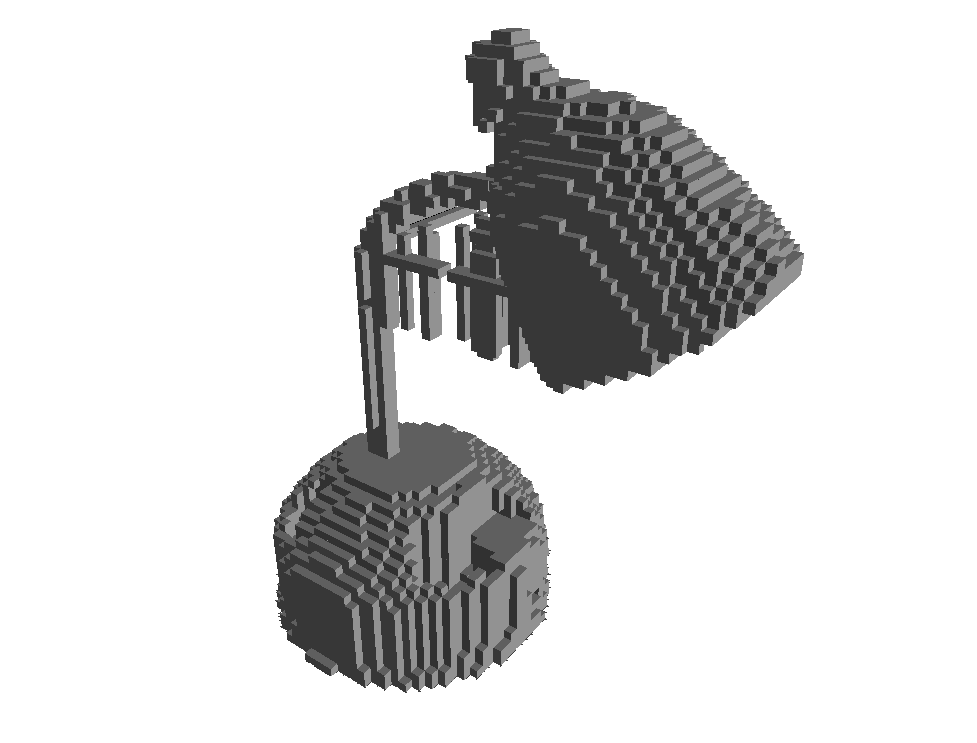
\includegraphics[width=\textwidth]{images/lamp_discrete}
		\caption{Die von binvox diskretisierte Version der Lampe}
	\end{subfigure}
	\caption{Das Tool binvox bei der Arbeit.}
\end{figure}

\section{Fallender Schnee}
\label{sec:implementation_snowflake}

\subsection{Schnee in interaktiven Anwendungen}

Aktuelle interaktive Anwendungen wie Spiele simulieren typischerweise
weder die Bildung einer Schneedecke noch den Fall von Schneeflocken in
physikalisch motivierter Art und Weise.

Für die Modellierung von Schneeflocken werden in Filmen und Spielen
oft lokale Modelle verwendet, die nicht auf ein (globales) Windfeld
zurückgreifen, sondern die Flocken lediglich in der Umgebung der Kamera
unter Zuhilfenahme von Zufallsvariablen simulieren. Es folgen
Beispiele der eingesetzten Verfahren:

\begin{figure}[h]
	\begin{subfigure}[t]{0.4\textwidth}
		\centering
		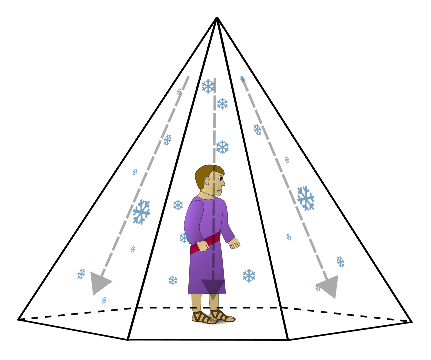
\includegraphics[width=\textwidth]{images/snow_double_cone}
                \caption{}
		\label{fig:introduction_snow_double_cone}
	\end{subfigure}
	~
	\begin{subfigure}[t]{0.6\textwidth}
		\centering
		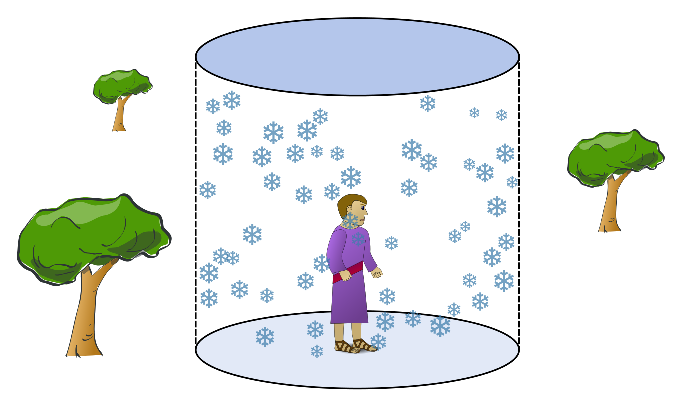
\includegraphics[width=\textwidth]{images/particle_cylinder}
                \caption{}
		\label{fig:introduction_particle_cylinder}
	\end{subfigure}
	\caption{(a) Schnee mittels Texturen, hier mit Hilfe eines Kegels um den Betrachter herum. Die Pfeile deuten an, dass die Texturen stetig nach unten gescrollt werden. (b) Ein lokales Modell für die Visualisierung von Schneeflocken. Außerhalb des gezeigten Zylinders werden keine Flocken erstellt.}
\end{figure}

\begin{enumerate}
\item Es werden ein oder mehrere Texturen direkt vor dem Auge des
Betrachters eingeblendet. Die Texturen stellen Bilder verschiedener
Schneeflocken dar und werden stetig nach unten bewegt um den Eindruck
zu erwecken, die Flocken fielen zu Boden.

Die zu den Texturen gehörige Geometrie ist entweder ein Rechteck
direkt vor dem Auge des Betrachters (eine texturierte
\PimiddyQuotes{Glasscheibe}, die sich mit dem Betrachter mitbewegt),
oder eine komplexere Form wie ein Kegel oder ein Doppelkegel (siehe
\cite{Wang2004}). Dieser Ansatz ist extrem eingeschränkt, denn der
Blickwinkel darf sich nicht signifikant von einem Horizontalen
unterscheiden. Er bietet sich dort an, wo die synthetische Kamera
ohnehin nicht frei ist, \PimiddyzB bei einem Flugsimulator.
\item Es wird ein \PimiddyBegriff{Partikelsystem}
verwendet\cite{Reeves:1983:PST:357318.357320}, also jede Schneeflocke
einzeln modelliert und weiterbewegt, was physikalisch wesentlich
akkurater ist. Dazu wird meist eine feste Anzahl an Schneeflocken
vorgegeben. Die Anzahl richtet sich nach der Rechnerleistung und der
Stärke des Schneefalls.

Die Partikel haben Eigenschaften wie eine Position, eine Masse und
eine Momentangeschwindigkeit, die am Anfang der Simulation zufällig
festgelegt werden. Als Position wird allerdings kein beliebiger,
zufälliger Punkt im Raum verwendet. Vielmehr wird ein Vektor
generiert, der sich innerhalb eines eingeschränkten Bereiches um den
Betrachter herum befindet, \PimiddyzB ein Punkt in einem Zylinder um
den Betrachter (vgl. \autoref{fig:introduction_particle_cylinder}).

Die Flocken werden auf Grund ihrer Geschwindigkeit
weiterbewegt. Treffen sie auf dem Boden auf, werden sie neu in die
Simulation gesetzt, wobei die Position wieder aus dem Zylinder gewählt
wird. Die Geschwindigkeit wird anhand der Schwerkraft verändert.  Hat
man zudem ein globales Schneemodell zur Verfügung, kann man die
Flugbahn der Flocken im Zylinder der Windgeschwindigkeit anpassen.

Problematisch ist die Behandlung von Hindernissen. Bewegt sich der
Betrachter beispielsweise in ein Gebäude, sollte bei geschlossener
Decke kein Schnee mehr um die Person generiert werden. Dies muss
gesondert behandelt werden. Eine ähnliche Situation ergibt sich, wenn
der Betrachter auf der windabgewandten Seite eines Gebäudes
steht. Hier sollten ebenfalls keine Schneeflocken generiert werden
(oder sehr wenige). Die ist nur sehr schwer umzusetzen, da der
Zylinder in seiner Größe begrenzt ist und wenn sonst ad hoc keine
Informationen über die Verteilung von Schnee in der Welt zur Verfügung
stehen.

Mit dieser Simulationsmethode lässt sich zudem keine Schneedecke
generieren. Es ist zwar möglich, den Auftreffpunkt der Schneeflocken
auf den Hindernissen weiterzuverarbeiten. Die so generierte
Schneedecke existiert aber nur in einer Umgebung um den Bewegungspfad
des Betrachters. Weiter entfernte Objekte sind stets frei von
Schnee.
\end{enumerate}

Wegen der besseren physikalischen Modellierbarkeit und wegen des
beliebig wählbaren Blickwinkels bei einer Ego-Perspektive wurde
entschieden, ein \emph{globales} Partikelsystem umzusetzen. Die
Flocken werden also anfänglich im gesamten Simulationsbereich
verteilt. Ihre Geschwindigkeit wird aufgrund der Windgeschwindigkeit
verändert. Das Auftreffen auf Hindernissen wird für die Schneedecke
weiterverarbeitet und die Flocke wird wieder an einen beliebigen,
zufälligen Ort gesetzt.

\subsection{Hintergründe}

Schnee ist, genau wie Regen, eine Spezialform von \PimiddyBegriff{Niederschlag}.
Hier soll kurz auf die Entstehung von Niederschlag und die Bildung von
Schneeflocken eingegangen werden. Der Erklärungsansatz orientiert sich
an \cite{wiki:Luftfeuchtigkeit}.

Überall dort, wo sich eine freie Wasseroberfläche wie z.\,B.\ ein See befindet und
die Temperatur einen bestimmten Wert übersteigt, lösen sich Moleküle der
Wasseroberfläche von ihrem Verbund und verdunsten in die Luft. Umgekehrt treffen
verdunstete Wassermoleküle wieder auf die Wasseroberfläche und kondensieren
dort. Die \emph{Kondensationsrate} und die
\emph{Verdunstungsrate} geben an, wie viel Wasser in einem Bereich zu
einem Zeitpunkt verdunstet und wie viel kondensiert.

Stellt man sich eine Wasseroberfläche bei trockener Luft vor, so ist
die Kondensationsrate anfangs 0, da keine Wassermoleküle in der Luft
enthalten sind, die kondensieren können. Die Verdunstungsrate ist
bei einer ausreichend hohen Temperatur allerdings ungleich 0. Mit der
Zeit steigt so die Anzahl der Wassermoleküle in der Luft, die Luft
\PimiddyQuotes{sättigt} sich mit Wasser. Dadurch steigt wiederum die
Kondensationsrate. Bei gleich bleibenden Bedingungen gleichen sich
nach einiger Zeit die Kondensation und Verdunstung aneinander an.  Die
in diesem Gleichgewichtszustand vorliegende Konzentration von
Wassermolekülen in der Luft ist die
\PimiddyBegriff{Sättigungskonzentration} oder \PimiddyBegriff{maximale
Luftfeuchtigkeit}. Sie ist umso höher, je wärmer es ist, siehe
\autoref{fig:implementation_moist_air}. Umgangssprachlich sagt man
daher, warme Luft könne \PimiddyQuotes{mehr Wasser aufnehmen}.

\begin{figure}[ht]
\centering
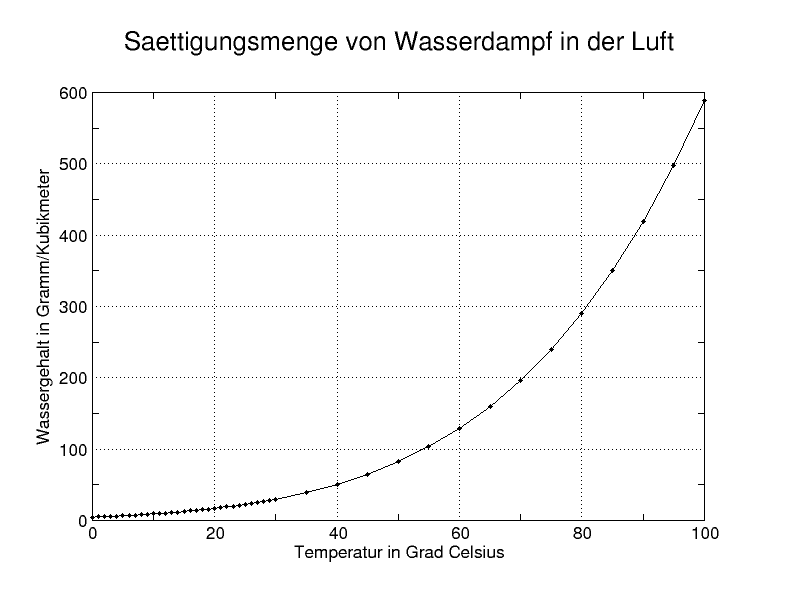
\includegraphics[width=15cm]{images/moist_air}
\caption{Der exponentielle Zusammenhang zwischen Temperatur und Sättigungsmenge von Wasserdampf in der Luft\cite{wiki:Saettigung}}
\label{fig:implementation_moist_air}
\end{figure}

Steigt warme Luft mit hoher Wassersättigung vom Boden in die
Atmosphäre auf, kann die Sättigungsmenge in den höheren Luftschichten
über den eigentlich maximalen Wert steigen -- es entsteht wieder ein
Ungleichgewicht. Um dieses Ungleichgewicht zu kompensieren, kondensiert
das überschüssige Wasser an sogenannten
\PimiddyBegriff{Kondensationskernen} (beispielsweise Staubpartikeln in
der Luft) und es bilden sich kleine Wassertröpfchen in
Mikrometergröße. Passiert dies großflächig, entstehen Wolken am
Himmel. Verdichten sich die kondensierten Tropfen weiter, werden sie
irgendwann zu schwer und fallen aufgrund der Schwerkraft herunter, es
entsteht \emph{Regen}.

Eine Spezialform der eben beschriebenen Kondensationskerne sind die
\emph{Kristallisationskerne}. Bei Temperaturen unter \PimiddyDegree{0}
bilden sich an diesen Kernen keine Tropfen sondern \emph{Kristalle}.
Bei starken Minustemperaturen (ab \PimiddyDegree{-40}) müssen sie
jedoch nicht vorhanden sein, es bilden sich auch so Kristalle.

Diese Kristalle sind anfangs noch sehr klein, sie wachsen erst während ihres
Falles zu Boden weiter an. Dabei entstehen aufgrund spezieller
Eigenschaften des Wassers charakteristische Formen, siehe
\autoref{fig:implementation_single_snow_crystal}. Durch die Verkettung
mehrerer Kristalle entstehen die Schneeflocken, die man beim
Zubodenfallen beobachten kann. Sie können eine Größe von bis zu 10cm
erreichen\cite{Nau96} und haben ebenfalls vielfältige Formen, die
allerdings keine Symmetrie mehr aufweisen, siehe
\autoref{fig:implementation_real_snowflakes}.

\begin{figure}
\centering
    \begin{subfigure}[t]{0.45\textwidth}
            \centering
            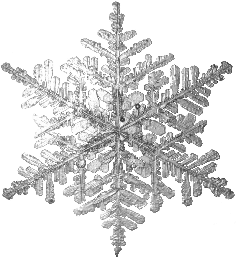
\includegraphics[width=\textwidth]{images/single_snow_crystal}
            \caption{Ein einzelner \PimiddyQuotes{Farn-artiger} Schneekristall\cite{Yanagi2011}.}
            \label{fig:implementation_single_snow_crystal}
    \end{subfigure}
    ~
    \begin{subfigure}[t]{0.45\textwidth}
            \centering
            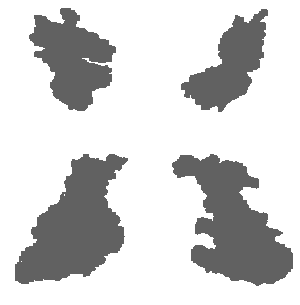
\includegraphics[width=\textwidth]{images/real_snowflakes}
            \caption{Kameraaufnahmen einzelner Schneeflocken mit etwa 1-2cm Durchmesser\cite{Hanesch1966}.}
            \label{fig:implementation_real_snowflakes}
    \end{subfigure}
\end{figure}

\begin{figure}[ht]
\centering
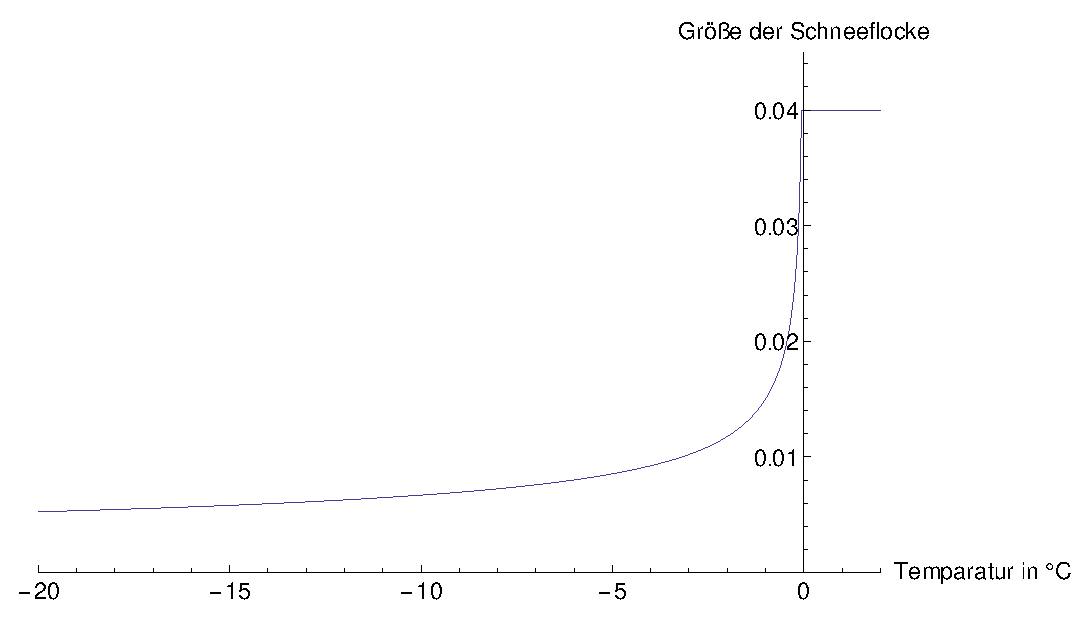
\includegraphics[width=14cm]{images/snowflake_size_graph}
\caption{Der Zusammenhang von Schneeflockengröße und Temperatur nach \cite{Jun00}.}
\label{fig:implementation_snowflake_size_graph}
\end{figure}

\subsection{Visualisierung}

Bei der Wahl der Visualisierungsmethode müssen mehrere Faktoren in
Betracht gezogen werden. Die Simulation soll sowohl ruhige
Wetterverhältnisse mit wenigen Schneeflocken als auch Szenen mit
starkem Wind und sehr vielen Schneeflocken behandeln können. Daher ist
einerseits wichtig, dass einzelne Schneeflocken einen gewissen
Detailgrad besitzen, aber die Performance gleichzeitig so wenig wie
möglich beeinträchtigen.

Es sollen mindestens die zwei wichtigsten Eigenschaften einer
Schneeflocke modelliert werden: die Größe und das Aussehen. Beide
Eigenschaften hängen von der Umgebungstemperatur ab. Für den Durchmesser $D$
einer Schneeflocke in Abhängigkeit von der Temperatur $T$ wurde in
\cite{Jun00} folgende Relation aufgestellt (siehe
\autoref{fig:implementation_snowflake_size_graph}):

\begin{equation}
\label{eq:implementation_snowflake_diameter}
D =
\begin{cases}
0.015 \cdot |T|^{-0.35} & \PimiddyFormelText{ für }T \leq -0.061 \\
0.04 & \PimiddyFormelText{ für }T > -0.061
\end{cases}
\end{equation}

Das Aussehen einer Schneeflocke bestimmt sich primär dadurch, ob
\emph{trockener} oder \emph{feuchter} Schnee vorliegt. Nahe bei
\PimiddyDegree{0} ist der Schnee feucht und hat eine hohe
Dichte. Bei kälteren Temperaturen werden die Schneeflocken kleiner und
sehen zarter aus.

Aagaard hat in \cite{Aagaard2004} ein Modell entwickelt, welches die
tatsächliche Form der Schneeflocke abhängig von Dichte und Größe
möglichst genau abbildet. Dazu verwendet er zufällig generierte, weiß
gefüllte Dreiecke, welche die Eiskristalle darstellen sollen. Anhand
des (randomisierten) Durchmessers der Schneeflocke wird eine Anzahl
von \emph{Schichten} ermittelt, in der die Dreiecke dann angeordnet werden,
siehe \autoref{fig:implementation_aagaard_layer_model} und
\autoref{fig:implementation_aagaard_spheres}. Auf diese Art können
vielfältige zufällige Formen generiert und an die aktuellen
Wetterbedingungen angepasst werden. Durch die dreidimensionale
Modellierung kann man den Flocken außerdem eine Rotation geben und sie
von allen Seiten betrachten.

Allerdings ist das Modell sehr laufzeitintensiv. Dies hat zwei Ursachen:

\begin{enumerate}
\item Die einzelnen Dreiecke einer Schneeflocke sind
halbtransparent. Dies führt dazu, dass weit mehr Fragments erzeugt
werden als es Pixel auf dem Bildschirm gibt. Diesen Effekt nennt man
\emph{Overdraw}.
\item Es werden Außerdem sehr sehr viele kleine Dreiecke für eine einzelne
Flocke benötigt (Aagaard geht von mindestens 10 aus, maximal über
100). Für 1.000 Flocken erhält man so schon 10.000 Dreiecke. Die
angestrebte Flockenzahl bei heftigem Schneefall liegt aber bei weit
über 1.000 Flocken. Aagaard schlägt daher vor, ein \PimiddyQuotes{Level
of detail}-System einzubauen, bei dem weiter entfernte Flocken durch
simplere Geometrie (z.\,B.\ mit weniger Dreiecken) angenähert werden. Er
implementiert dies jedoch selber nicht, da Performance kein
entscheidender Faktor für die Implementierung ist.
\item Die Eigenschaften einer Schneeflocke wie etwa ihre Geschwindigkeit
und die Darstellung der Flocke müssen getrennt werden, da OpenGL es
nicht direkt erlaubt, Daten für einen \PimiddyQuotes{Block} von
Primitiven anzugeben wie etwa die Dreiecke der Schneeflocke. Dies
macht die Implementierung schwieriger und langsamer.
\end{enumerate}

\begin{figure}[ht]
    \centering
    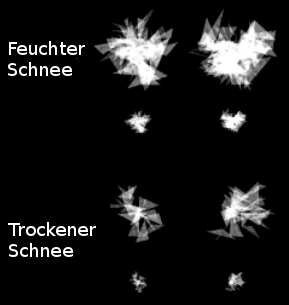
\includegraphics{images/aagaard_layer_model}
    \caption{Das Resultat von Aagaards 3D-Modell für die Schneeflocken.}
    \label{fig:implementation_aagaard_layer_model}
\end{figure}

\begin{figure}[ht]
    \centering
    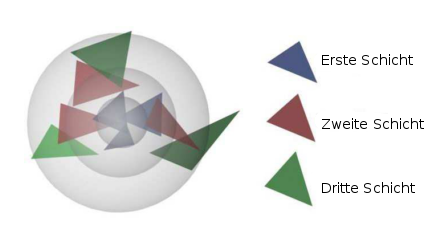
\includegraphics{images/aagaard_spheres}
    \caption{Der schichtweise Aufbau einer Schneeflocke in Aagaards Modell.}
    \label{fig:implementation_aagaard_spheres}
\end{figure}

\begin{figure}[ht]
    \centering
    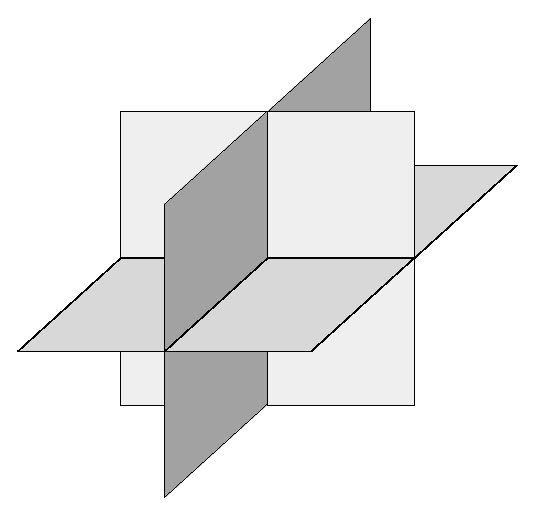
\includegraphics{images/snowflake_three_rectangles}
    \caption{Eine Schneeflocke aus drei Rechtecken zusammengesetzt.}
    \label{fig:implementation_snowflake_three_rectangles}
\end{figure}

In \cite{Saltvik2006} findet sich ein etwas simplerer Ansatz, der nur
drei transparente Rechtecke pro Schneeflocke verwendet (siehe
\autoref{fig:implementation_snowflake_three_rectangles}). Dadurch wird
massiv Performance gespart, die Daten für die Flocken müssen
allerdings trotzdem in einem separaten Buffer gespeichert werden.

In dieser Arbeit wird stattdessen eine simplere Visualisierung mit
Hilfe von sogenannten \PimiddyBegriff{Pointsprites} gewählt. Statt
mehrerer Dreiecke repräsentiert nur ein einzelner Punkt eine
Schneeflocke. Dadurch wird es möglich, alle Daten für eine Flocke im
OpenGL-Buffer selber zu speichern. Zudem sind Punkte in OpenGL sind
allerdings mathematischen Punkte, denn sie besitzen eine
\emph{Ausdehnung}. Dadurch wird es möglich, die Flockengröße zu variieren.

Diese Ausdehnung jedoch nicht in Weltkoordinaten angegeben, sondern in
Pixeln auf dem Bildschirm. Das bedeutet, dass die Flocken immer zum
Betrachter zeigen, man kann sich nicht um sie herum bewegen (siehe
\autoref{fig:implementation_point_sprite_vs_billboard}). Außerdem muss
-- im Gegensatz zu Dreiecken -- eine Formel für die Größe erdacht
werden, damit weiter entfernte Punkte kleiner werden (für Dreiecke
wird dies mit Hilfe einer perspektivischen Projektionsmatrix
sichergestellt).

\begin{figure}[ht]
    \centering
    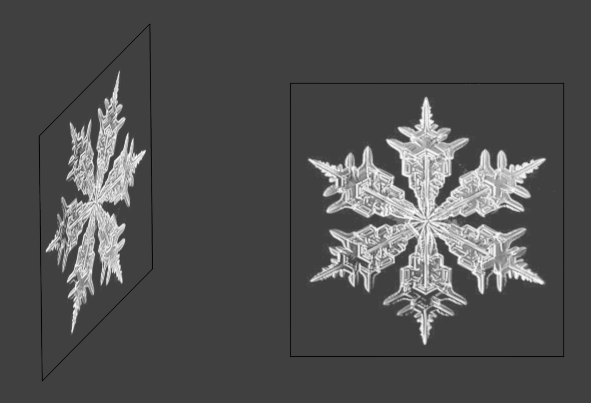
\includegraphics{images/point_sprite_vs_billboard}
    \caption{Links ein Schneekristall aus zwei Dreiecken zusammengesetzt, rechts als Pointsprite.}
    \label{fig:implementation_point_sprite_vs_billboard}
\end{figure}

\begin{listing}
\begin{minted}{glsl}
uniform mat4 model_view_projection;
uniform vec4 eye_position;

in vec4 position;
in float point_size;

float determine_point_size(float distance_to_camera)
{
   // ...
}

void main()
{
  float distance_to_camera = distance(eye_position,position);
  gl_PointSize = determine_point_size(distance_to_camera);
  gl_Position = model_view_projection * position;
}
\end{minted}
\caption{Der zu Pointsprites gehörige Vertexshader}
\label{lst:implementation_point_sprite_vertex_shader}
\end{listing}

\begin{listing}
\begin{minted}{glsl}
uniform sampler2D snowflake_texture;

out vec4 fragment_color;

void main()
{
  // Einfarbige Punkte (hier weiss)
  // fragment_color = vec4(1.0,1.0,1.0,1.0);
  // Mit Textur:
  fragment_color = texture(snowflake_texture,gl_FragCoord);
}
\end{minted}
\caption{Der zu Pointsprites gehörige Fragmentshader}
\label{lst:implementation_point_sprite_fragment_shader}
\end{listing}

Um Pointsprites in OpenGL zu zeichnen, gibt man bei der OpenGL-Funktion
\PimiddyInlineCode{glDrawArrays} den Primitvtyp
\PimiddyInlineCode{GL\_POINTS}
an. \PimiddyListingRef{lst:implementation_point_sprite_vertex_shader}
zeigt den dazugehörigen Vertexshader, der als Input die
Projektionsmatrix, den Augenpunkt, die Größe der Schneeflocke und
deren Position bekommt. Mit Hilfe der Variable
\PimiddyInlineCode{gl\_PointSize}, der man einen
\PimiddyInlineCode{float}-Wert zuweist, kann man die Größe des Punktes
setzen. Die Funktion \PimiddyInlineCode{determine\_point\_size} wird
gleich erläutert.

Der zu
\PimiddyListingRef{lst:implementation_point_sprite_vertex_shader}
gehörige Fragmentshader
\PimiddyListingRef{lst:implementation_point_sprite_fragment_shader}
verwendet den zweidimensionalen Vektor
\PimiddyInlineCode{gl\_FragCoords} $\in [0,1]^2$. Dieser Vektor gibt
an, wo sich das Fragment innerhalb des aktuellen Punktes (respektive,
der aktuellen Flocke) befindet. OpenGL verwaltet also ein eigenes
Koordinatensystem innerhalb des Punktes. Mit Hilfe dessen kann man den
Punkten im Fragmentshader nicht nur eine einheitliche Farbe geben,
sondern auch eine Textur. Die Textur der Punkte wird in der
Implementierung zufällig aus einer Menge von Texturen ausgewählt, die
zur aktuellen Außentemperatur passen.

Um den Vertexshader zu komplettieren, muss noch die Größe der
Pointsprites bestimmt werden. Verwendet man für seine Szene eine
perspektivische Projektion, besteht zwischen dem Abstand von Objekten
und ihrer dargestellten Größe ein nichtlinearer Zusammenhang. Daher
sollte auch für die Größe der Pointsprites eine ähnliche
Proportionalität bestehen. Microsofts DirectX-Framework verwendet
hierfür folgende
Formel\cite{DirectXPointSprites}:

\begin{equation}
\label{eq:implementation_snowflake_perspective_formula}
S =
S'
\sqrt{
  \frac
  {
    1
  }
  {
    A +
    B \cdot D_e +
    C \cdot D_e^2
  }
}
\end{equation}

$S'$ bezeichnet hierbei die vorgegebene Punktgröße, die Konstanten
$A,B,C$ sind frei wählbar und $D_e$ bezeichnet den Abstand des Punktes
von der Kamera. Die Werte $A=0.96,B=0.19,C=0.06$ haben sich als
visuell ansprechend herausgestellt.

Für die Simulation von heftigem Schneefall reicht es allerdings nicht
aus, nur die Anzahl der Flocken zu erhöhen und deren Größe zu
randomisieren. Das menschliche Auge interpretiert die Flocken dann
eher als unrealistisches \PimiddyQuotes{Rauschen}. Um dies auszumerzen
wird in \cite{Langer2004} wird ein Verfahren vorgestellt, mit dem in
der Bildebene aus einigen wenigen Schneeflocken weitere synthetisiert
werden, sodass ein realistischer Eindruck einer großen Menge
Schneeflocken entsteht. Dieses Verfahren ist sehr performant,
allerdings relativ schwierig umzusetzen. Daher wurde ein anderer Weg
gewählt, nämlich die \emph{Transparenz} der Schneeflocken ebenfalls
abhängig von der Entfernung zur Kamera mit Hilfe von
\autoref{eq:implementation_snowflake_perspective_formula} zu
variieren, allerdings mit den Konstanten $A=0.1,B=0.15,C=0$ und
$S'=1$.

Mit Hilfe von Pointsprites ist es möglich, auf einem aktuellen System
weit über 100.000 Schneeflocken gleichzeitig anzuzeigen. Es ist jedoch
nicht möglich, die Flocken rotieren zu lassen, was allerdings visuell
nicht kritisch ist.

\subsection{Modellierung}

\subsubsection{Einleitung}

Nach der visuellen Beschreibung der Schneeflocken soll nun deren
Bewegung erläutert werden. Dazu wird zuerst ein physikalisch
motiviertes Modell eingeführt und danach die Implementierungsdetails
des Partikelsystems erklärt.

Physikalisch gesehen wird eine Schneeflocke als \emph{starrer Körper}
mit einer sehr geringen Masse modelliert. Kennt man die aktuelle
Geschwindigkeit $\vec{v}$ des Körpers, sowie seine momentane Position
$\vec{p}$ und hat man ein Zeitdelta $\Delta t$ gegeben, dann kann
seine Bahn $\vec{s}$ in diesem Zeitschritt durch das
\emph{Weg-Zeit-Gesetz} bestimmt werden, sofern man die momentane
Beschleunigung $\vec{a}$ kennt:

\begin{equation}
\label{eq:implementation_snowflake_path_time_law}
\vec{s} = \frac{1}{2} \vec{a} \Delta t^2 + \vec{v}t + \vec{p}
\end{equation}

Dabei nimmt man natürlich an, die Beschleunigung sei in dem
Zeitabschnitt $\Delta t$, den man grade betrachtet, konstant. Für die
Beschleunigung selber gilt Newtons Formel:

\begin{gather}
\vec{F} = m \cdot \vec{a} \\
\vec{a} = \frac{\vec{F}}{m}
\end{gather}

Man muss also -- wie schon beim Windfeld -- berechnen, welche Kräfte
auf die Schneeflocke wirken. Daraus ergibt sich dann die Flugbahn. Es
bietet sich manchmal auch an, eine Kraft nicht als Beschleunigung zu
modellieren, sondern sie in
\autoref{eq:implementation_snowflake_path_time_law} direkt auf die
Geschwindigkeit zu addieren (die Geschwindigkeit der Schneeflocke also
nicht zu verändern). Im Folgenden sollen die einzelnen Kräfte
näher beleuchtet werden.

In \cite{Aagaard2004} wurden vier Kräfte zusammengetragen, welche
zusammen die Bewegung einer Schneeflocke beeinflussen:

\begin{enumerate}
\item Die Schwerkraft $\vec{F}_g$ ist eine konstante Kraft, die
-- genau wie beim Windfeld -- in negativer $y$-Richtung wirkt.
\item Der Wind übt eine Kraft $\vec{F}_\PimiddyFormelText{w}$
auf die Schneeflocke aus, die den \PimiddyBegriff{Luftwiderstand}
widerspiegelt. Aufgrund der geringen Masse der Flocken ist dies die
Kraft, welche die Flocke am meisten in ihrer Bahn beeinflusst.
\item Die aerodynamische Form der Flocke führt dazu, dass sie selbst bei
Windstille keine direkte Bahn zum Boden verfolgt, sondern in kleinen
Spiralbahnen zur Erde fällt. Dieser Effekt wird
\PimiddyBegriff{dynamischer Auftrieb} genannt. Er wird jedoch nicht
als Kraft modelliert, sondern direkt als Geschwindigkeitsänderung (siehe unten).
\item Auch Schneeflocken haben einen gewissen \emph{statischen
Auftrieb} $F_{\PimiddyFormelText{Auftrieb}}$ innerhalb der umgebenden
Luft.
\end{enumerate}

Diese Kräfte werden nun einzeln besprochen. Es werden
OpenCL-C-Funktionen aufgestellt, die die Kräfte abhängig von den
Eigenschaften einer Schneeflocke umsetzen. Diese Funktionen werden
schließlich in dem Kernel, der die Schneeflocken weiterbewegt,
benutzt.

\subsubsection{Luftwiderstand}

Die Methode von Stam liefert ein dreidimensionales Vektorfeld von
Windgeschwindigkeiten. Das bedeutet, man kann in jedem Punkt innerhalb der
Simulationsgrenzen eine Windgeschwindigkeit angeben (wenn der Punkt
nicht auf dem Gitter liegt, wird stattdessen ein Geschwindigkeitswert
interpoliert).

Es ist aber noch nicht klar, welchen Einfluss die Windgeschwindigkeit
auf die Geschwindigkeit der Flocke ausübt, welche Kraft also aus der
Windgeschwindigkeit resultiert. Im Folgenden wird eine einzelne
Schneeflocke an Position $\vec{p}_f$ mit Geschwindigkeit $\vec{v}_{f}$
betrachtet. Mit $\vec{v}_w$ sei die Geschwindigkeit des Windes an
Position $\vec{p}_f$ bezeichnet.

Der Luftwiderstand -- oder allgemeiner der
\PimiddyBegriff{Strömungswiderstand} in Fluiden -- bezeichnet eine
Kraft, die ein Fluid der Bewegung eines Körpers entgegensetzt. Bei der
Berechnung dieser Kraft kommt es auf die \emph{Relativgeschwindigkeit}
von Schneeflocke und Wind an. Herrscht beispielsweise Windstille (ist
also $\vec{v}_w = 0$), sorgt die Schwerkraft für eine konstante
Beschleunigung nach unten, die Flocke fällt immer schneller zu Boden.

Der Luftwiderstand wirkt dieser Beschleunigung entgegen, und das umso
stärker, je schneller die Flocke ist. Dadurch stellt sich irgendwann
ein Gleichgewicht zwischen Schwerkraft und Luftwiderstand ein und die
Flocke erreicht ihre \PimiddyBegriff{Endgeschwindigkeit}
$v_{y,\PimiddyFormelText{max}}$. Im Vakuum hingegen könnte eine
Schneeflocke theoretisch beliebig schnell fallen.
\begin{figure}[ht]
    \centering
    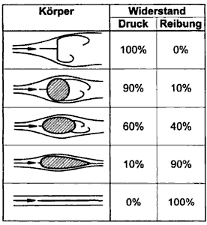
\includegraphics[width=10cm]{images/drag_forces}
    \caption{Der Zusammenhang von Druck- und Reibungswiderstand in Abhängigkeit der Form des umströmten Objekts.}
    \label{fig:implementation_snowflake_drag_forces}
\end{figure}

Streng genommen ist der Luftwiderstand aufgeteilt in
\PimiddyBegriff{Druckwiderstand} und
\PimiddyBegriff{Reibungswiderstand}. Deren Anteile hängen von der Form
des umströmten Körpers ab. Bei einer Kreisscheibe überwiegt der
Druckwiderstand, bei einer Tragfläche eines Flugzeugs beispielsweise
der Reibungswiderstand, siehe
\autoref{fig:implementation_snowflake_drag_forces}. Die Unterscheidung
spielt hier aber keine Rolle.

$\vec{v}_r$ bezeichne die Relativgeschwindigkeit von Flocke und Wind:
\begin{equation}
\vec{v}_r = \vec{v}_w - \vec{v}_f
\end{equation}
Der Luftwiderstand kann für Fluide mit hohen Geschwindigkeiten (die
Windgeschwindigkeit fällt in diese Kategorie) mit der folgenden
Luftwiderstandsformel angegeben werden, die auf \PimiddyName{Rayleigh}
zurückgeht:

\begin{equation}
\label{eq:implementation_snowflake_drag_equation}
\vec{F}_w = \frac{1}{2} \rho_{\PimiddyFormelText{Luft}} \vec{v_r^2} C_d A
\end{equation}

In der Formel bezeichnet $\rho_{\PimiddyFormelText{Luft}}$ die Dichte
der Luft, die bei \PimiddyDegree{0} etwa $1.293\frac{kg}{m^3}$
beträgt. $A$ bezeichnet die \emph{Bezugsfläche} des Körpers, den man
betrachtet. Nähert man die Schneeflocke als Kugel mit Radius $r$ an,
so kann $A$ als $\pi r^2$ gewählt werden, wenn man die Projektion der
Kugel auf die Ebene als Referenz wählt, oder $2\pi r^2$, wenn man die
\PimiddyQuotes{Vorderfläche} der Kugel als Referenz wählt. $C_d$
bezeichnet den dimensionslosen
\PimiddyBegriff{Strömungswiderstandkoeffizienten}.

Der Luftwiderstand wächst also quadratisch zur Geschwindigkeit des
Objekts. Dadurch, dass die Relativgeschwindigkeit $\vec{v}_r$ in die
Formel eingesetzt wurde, entsteht auch bei Windstille eine zur
Geschwindigkeit der Flocke entgegengesetzte Kraft.

Die Größen $C_d$ ist noch unbekannt. Sie wird normalerweise
experimentell ermittelt. Da zu diesem Thema jedoch keine Ergebnisse zu
finden sind, muss ein anderer Weg gewählt werden, um den Koeffizienten
abschätzen zu können.

Angenommen eine Schneeflocke fällt mit ihrer Endgeschwindigkeit
$v_{y,\PimiddyFormelText{max}}$ grade nach unten. Dann
entspricht die Kraft, die durch den Luftwiderstand hervorgerufen wird,
genau der Schwerkraft:
\begin{align}
\PimiddyBetrag{\vec{F}_g} &= \PimiddyBetrag{\vec{F}_w} \\
m \cdot \PimiddyBetrag{\vec{g}} &= \frac{1}{2} \rho v_{y,\PimiddyFormelText{max}}^2 C_d A
\end{align}
Löst man die untere Gleichung nach $C_d$ auf erhält man:
\begin{equation}
C_d
=
\frac
{
  2 \cdot m \cdot \PimiddyBetrag{\vec{g}}
}
{
  \rho \cdot v_{y,\PimiddyFormelText{max}}^2 \cdot A
}
\end{equation}
Dies eingesetzt in die Luftwiderstandsformel
\ref{eq:implementation_snowflake_drag_equation} ergibt:
\begin{equation}
\vec{F}_w =
\frac
{
  \vec{v_w^2} \cdot m \cdot \PimiddyBetrag{\vec{g}}
}
{
  v_{y,\PimiddyFormelText{max}}^2
}
\end{equation}
Die Formel hängt nur noch von $v_{y,\PimiddyFormelText{max}}^2$
ab. Diese Größe ist -- im Gegensatz zu $C_d$ -- gut bestimmt worden,
z.B.\ in \cite{Hanesch1966} für Temperaturen zwischen \PimiddyDegree{-2}
und \PimiddyDegree{0}. Dabei wurde festgestellt,
dass die Größe der Schneeflocke kaum Einfluss auf die
Fallgeschwindigkeit hat. Es wurden Geschwindigkeiten im Bereich $0.5m/s$
bis $2.0m/s$ gemessen. In
\cite{Centre1998} wurde festgestellt, dass zwischen feuchtem und
trockenen Schnee ein Faktor 2 bezüglich der Geschwindigkeit
besteht. Aagaard wählt in \cite{Aagaard2004} daher die folgenden
Endgeschwindigkeiten:
\begin{align}
0.5 \frac{m}{s} \leq v_{y,\PimiddyFormelText{max},\PimiddyFormelText{trocken}} \leq 1.5 \frac{m}{s} \\
1 \frac{m}{s} \leq v_{y,\PimiddyFormelText{max},\PimiddyFormelText{feucht}} \leq 2 \frac{m}{s}
\end{align}
Um $\vec{F}_w$ zu bestimmen, muss nun lediglich die Masse $m$ der
Schneeflocke untersucht werden. In \cite{Centre1998} wurde
festgestellt, dass sich die \emph{Dichte} einer Schneeflocke etwa
umgekehrt proportional zu ihrem Durchmesser verhält:
\begin{align}
\rho_{\PimiddyFormelText{Flocke}} = \frac{1}{D}
\end{align}
Der Durchmesser einer Flocke wurde bereits behandelt. Zwischen
Dichte und Masse besteht die Beziehung $\rho = m \cdot V$, wobei $V$
das Volumen des betrachteten Körpers ist. Es wird daher $\rho = m$
gesetzt.

Damit lässt sich $\vec{F}_w$ nun vollständig bestimmen. Wie später
erläutert wird, werden für den Querschnitt $A$ der Flocken, sowie für
$v_{y,\PimiddyFormelText{max}}$ zufällige Werte bestimmt, um ein
natürlicheres Muster zu erzeugen und um die Annäherung der Flocken
durch Kugeln auszugleichen. Die folgende Funktion setzt den Kernel die
Kraft um, die durch den Luftwiderstand erzeugt wird:

\begin{minted}[frame=lines]{c}
float3 drag_force(
    float3 terminal_velocity,
    float diameter,
    float3 wind_velocity,
    float3 flake_velocity,
    float gravity)
{
    return
        // Quadrierte Relativgeschwindigkeit
        pow(wind_velocity - flake_velocity,2.0f) *
        // Annaeherung fuer die Masse
        (1.0f / diameter) *
        gravity /
        pow(terminal_velocity,2.0f);
}
\end{minted}

\subsubsection{Dynamischer Auftrieb}

Beobachtungen an Schneeflocken bei ruhigem Wetter haben ergeben, dass
die Flocken selten in einer geraden Bahn nach unten fallen, sondern
eher \PimiddyQuotes{Zick-Zack-Bewegungen} machen, siehe
\autoref{fig:implementation_snowflake_helix}.

\begin{figure}[ht]
    \centering
    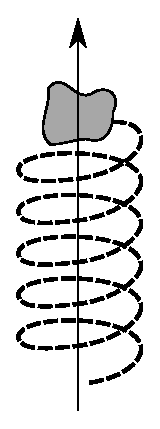
\includegraphics{images/snowflake_spiral}
    \caption{Die ungefähre Bahn eine Schneeflocke ohne den Einfluss von Wind.}
    \label{fig:implementation_snowflake_helix}
\end{figure}

Diese Spiralbahn kann nicht durch den Luftwiderstand hervorgerufen
werden, denn dieser wirkt bei Windstille nur entgegengesetzt der
Schwerkraft, also grade nach oben. Stattdessen wird eine Kraft dadurch
erzeugt, dass sich hinter der Schneeflocke Verwirbelungen bilden und
sie dadurch orthogonal zur Flugbahn ablenken, siehe
\autoref{fig:implementation_snowflake_vortex_shedding}. Dasselbe
Phänomen tritt auch makroskopisch in der Atmosphäre auf, siehe
\autoref{fig:implementation_snowflake_vortex_shedding_macroscopic}.

\begin{figure}[ht]
    \centering
    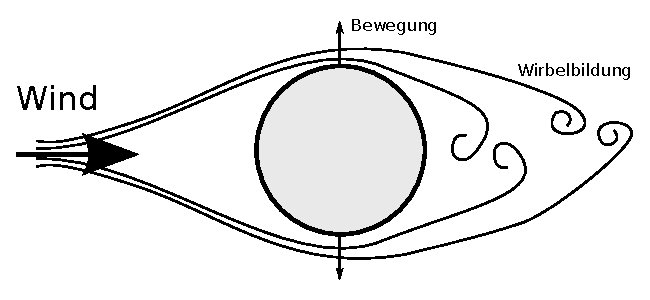
\includegraphics{images/vortex_shedding}
    \caption{Hinter der Schneeflocke bilden sich während des Flugs Wirbel, die eine Kraft seitwärts ausüben.}
    \label{fig:implementation_snowflake_vortex_shedding}
\end{figure}

\begin{figure}[ht]
    \centering
    \includegraphics{images/vortex_shedding_macroscopic}
    \caption{Die Insel Rishiri-to an der nordwestlichen Küste von Hokkaido, Japan erzeugt Wirbel in der Atmosphäre, die sich über weite Strecken ausbreiten.}
    \label{fig:implementation_snowflake_vortex_shedding_macroscopic}
\end{figure}

Die Wirbel entstehen durch niedrigen Druck, der hinter dem Hindernis
entsteht. Je nach Form des Objekts hat er unterschiedliche
Auswirkungen. Der dynamische Auftrieb auf dünnen, länglichen Objekten
wie den Tragflächen von Flugzeugen sorgt dafür, dass das Flugzeug
abhebt. Er ermöglicht Vögeln und Flugzeugen das Fliegen. Bei stumpfen
Körpern wie Golfbällen oder Schneeflocken hingegen bilden sich die
besagten Wirbel und dadurch eine Seitwärtsbewegung. Diese Wirbel sind
im dreidimensionalen nur sehr schwer zu beschreiben. Statt einem
genauen Modell wird also ein einfacheres Modell angesetzt und der
Effekt nur \PimiddyQuotes{nachgebaut}.

Damit die Schneeflocke sich auf einer kreisförmigen Bahn in der
$xz$-Ebene bewegt, legen wir folgende Ablenkungsgeschwindigkeit zugrunde:

\begin{equation}
\label{eq:implementation_snowflake_lift_velocity}
\vec{v}_{a} =
\omega \cdot r
\left(
\begin{array}{c}
-\sin{\omega t} \\
0 \\
\cos{\omega t}
\end{array}
\right)
\end{equation}

Hier bezeichnet $\omega$ die Winkelgeschwindigkeit, $r$ den
Kreisradius der Bahn und $t$ den Zeitparameter (in diesem Fall kein
Zeitdelta, sondern ein absoluter Wert). Die Flocken sollen allerdings
nur dann eine Kreisbahn einnehmen, wenn ihre Geschwindigkeit relativ
wenig durch den Wind beeinflusst wird. Deshalb wird die
\autoref{eq:implementation_snowflake_lift_velocity} mit einem $C_a$
gewichtet:

\begin{equation}
C_a =
\frac
{
  \PimiddyBetrag{\vec{v}_w - \vec{v}_f}
}
{
  \PimiddyBetrag{\vec{v}_f}
}
\end{equation}

Es wurden keine Experimente bezüglich des Bahnradius $r$ und der
Winkelgeschwindigkeit $\omega$ gefunden. Experimentelle Werte ergeben
aber für diese Größen folgende Einschränkungen:

\begin{gather}
-\frac{\pi}{4} \leq \omega \leq -\frac{\pi}{3} \\
0 \leq r \leq 2
\end{gather}

Auch diese Größen werden also randomisiert. Die folgende Funktion gibt
die Geschwindigkeitskorrektur durch den dynamischen Auftrieb an:

\begin{minted}[frame=lines]{c}
float3 lift_force(
    float3 wind_velocity,
    float3 flake_velocity,
    float angular_velocity,
    float radius,
    float t)
{
    return
        length(wind_velocity - flake_velocity) / length(flake_velocity) *
        angular_velocity * radius *
        (float3)(
            -sin(angular_velocity * t),
            0.0f,
            cos(angular_velocity * t));
}
\end{minted}

\subsubsection{Statische Auftrieb}

Auftrieb bezeichnet eine Kraft, die der Schwerkraft entgegengesetzt
ist. Sie wirkt also in Richtung $(0,1,0)$. Sie entsteht durch die
Verdrängung des Fluids durch einen Körper und sie ist indirekt
abhängig von der Luftdichte. Sei daher
$\rho_{\PimiddyFormelText{Luft}}(x,y,z)$ das Vektorfeld der Dichte in
jedem Punkt. Es ergibt sich bei $(x,y,z)$ der folgende (betragsmäßige)
Auftrieb:

\begin{equation}
|F_A| = \rho_{\PimiddyFormelText{Luft}}(x,y,z) \cdot V \cdot g
\end{equation}

Hier ist $V$ das Volumen der Schneeflocke und $g$ die
Gravitationskonstante. Dieser Zusammenhang ist als
\emph{Archimedisches Prinzip} bekannt.

Aus folgenden Gründen wurde sich allerdings \emph{dagegen}
entschieden, den statischen Auftrieb zu modellieren:

\begin{enumerate}
\item Die Dichte der Luft ist abhängig vom Druck und von der
Temperatur. Die Temperatur wird allerdings nicht explizit
modelliert, man kann sie also überall als konstant annehmen. Der Druck
variiert verhältnismäßig wenig. Daher kann insgesamt die Dichte der
Luft als konstant angenommen werden. Die Auftriebskraft variiert so
nur mit dem (ebenfalls sehr kleinen) randomisierten Volumen der
Schneeflocken.
\item Die Dichte der Luft ist nicht nur konstant, sie ist auch sehr
klein im Vergleich zu anderen Fluiden wie z.\,B.\ Wasser, was den
Effekt von Auftrieb vernachlässigbar macht.
\end{enumerate}

\subsubsection{Code}

\begin{table}[H]
	\caption{Die zu einer Flocke gehörigen Daten und ihr Ursprung}
	\centering
	\begin{tabular}{@{}cm{5cm}m{7cm}@{}}
		\toprule \\
                \PimiddyTableHeading{E}
		&
                \PimiddyTableHeading{Beschreibung}
                &
                \PimiddyTableHeading{Berechnung} \\
		\midrule \\
			$\vec{p}$
		&
                        Position
		&
                        Zufälliger Anfangswert innerhalb der Simulationsgrenzen
		\\
			$\vec{v}$
		&
                        Geschwindigkeit
		&
                        Anfangs gleich $v_{y,\PimiddyFormelText{max}}$
		\\
			$D$
		&
                        Durchmesser der Flocke
		&
                        Gemäß \autoref{eq:implementation_snowflake_diameter}
		\\
			$r$
		&
                        Rotationsradius für dynamischen Auftrieb
		&
                        Zufällig, gleichverteilt aus dem Intervall $[0,2]$
		\\
			$\omega$
		&
                        Winkelgeschwindigkeit für dynamischen Auftrieb
		&
                        Zufällig, gleichverteilt aus dem Intervall $[-\pi/4,-\pi/3]$ oder $[\pi/4,\pi/3]$
		\\
			$v_{y,\PimiddyFormelText{max}}$
		&
                        Endgeschwindigkeit
		&
                        Zufällig, gleichverteilt aus $[0.5,1.5]$ für feuchten Schnee bzw.\ $[1.0,2.0]$ für trockenen Schnee.
		\\
		\\
		\bottomrule
	\end{tabular}
	\label{table:implementation_snowflake_properties}
\end{table}

Nun wird die konkrete Umsetzung der Partikelsimulation
besprochen. \autoref{table:implementation_snowflake_properties} zeigt
die Eigenschaften, die für jede Flocke zu verwalten sind. Viele dieser
Eigenschaften wie die Größe oder der Rotationsradius können einmalig
beim Erstellen des Buffers auf dem Host gesetzt werden und bleiben
dann konstant, sofern die Außentemperatur $T$ nicht verändert
wird. Dynamisch sind einzig die Eigenschaften Position und
Geschwindigkeit. Für jede Eigenschaft wird ein Buffer auf der
Grafikkarte reserviert.

Die Bewegung der Schneeflocken ist in zwei Teile geteilt, den
\emph{Bewegungsteil} und den \emph{Kollisionsteil}, die allerdings aus
Performancegründen später in einem einzigen Kernel umgesetzt sind.

Die Methode für die Bewegung der Flocken bekommt als weitere Eingabe
das Vektorfeld der Geschwindigkeitspfeile. Daraus wird die
Geschwindigkeit des Fluids an der Position der Flocke
interpoliert. Weiterhin wird ein fortlaufender Zeitparameter
\PimiddyInlineCode{t} zusätzlich zum Zeitdelta \PimiddyInlineCode{dt}
an den Kernel gegeben. Mit \PimiddyInlineCode{t} wird die Rotation der
Flocke berechnet.

Nach Ausführung der Bewegungsmethode kann es allerdings vorkommen,
dass eine Flocke entweder in einem Hindernis oder außerhalb des
Simulationsbereiches landet. In diesem Fall muss eine neue Position
für die Schneeflocke gefunden werden. Hier ergeben sich zwei
Schwierigkeiten:

\begin{enumerate}
\item Die neue Position sollte zufällig gewählt werden, damit ein
minimaler Grad an sich wiederholenden Mustern beim Schneefall
auftreten. Die Grafikkarte bietet jedoch keinen Mechanismus hierfür,
weder für Pseudozufallszahlen noch für echten Zufall.
\item Die neue Position sollte idealerweise nicht so gewählt werden,
dass sie wieder in einem Hindernis liegt.
\end{enumerate}

Da kein Mechanismus in OpenCL vorhanden ist, um Zufallszahlen zu
generieren, müssen die im Kernel schon verfügbaren Daten als
Zufallsquelle herangezogen werden. OpenCL schreibt vor, dass Zahlen
vom Typ \PimiddyInlineCode{float} im IEEE-754-Format vorliegen
müssen. Dies erlaubt es, Eigenschaften dieser Kodierung auszunutzen,
um für einen gegebenen Fließkommawert einen pseudozufälligen Wert
zurückzugeben, der aus den einzelnen Bits der Eingabezahl
entsteht. Dies wurde in \cite{Eidissen2009} in CUDA umgesetzt, um die
Positionen von Partikeln zu randomisieren. Die folgende
OpenCL-C-Funktion gibt einen Wert im Intervall $[0,1]$ zurück.

\begin{minted}[frame=lines]{c}
float
random_float_value(
    float f)
{
    return
        (as_float(
             as_int(f) & 0x007fffff | 0x40000000)
         - 3.0f
         + 1.0f) /
        2.0f;
}
\end{minted}

Die Eingabe \PimiddyInlineCode{f} zeitweise als Ganzzahl interpretiert, um
die Bit-Operatoren \PimiddyInlineCode{\&} und \PimiddyInlineCode{|}
auszunutzen.

Diese Funktion kann man jetzt nutzen, um gegeben der alten Position
der Schneeflocke eine neue Position zu finden. Der folgende Code
enthält die Funktion, um eine neue Position zu berechnen sowie um eine
gegebene Flocke zurückzusetzen.

\begin{minted}[frame=lines]{c}
float3
random_position(
    int4 bounding_rect,
    float3 f)
{
    float3 result;

    result.x =
        random_float_value(
            (f.x + f.z) / f.y);
    result.z =
        random_float_value(
            f.x / f.z + f.y);
    result.y =
        result.x +
        (1.0f - result.x) *
        random_float_value(
            f.x - f.z - f.y);

    return
        result *
        convert_float3(
            bounding_rect);
}

void
reset_flake(
    global float3 *positions,
    global float3 *velocities,
    global float *terminal_velocities,
    int3 bounding_volume,
    size_t my_id)
{
      positions[my_id] = random_position(bounding_volume,positions[my_id]);
      velocities[my_id] = (float3)(0.0f,-terminal_velocities[my_id],0.0f);
      return;
}
\end{minted}

Statt nur der alten Position der Schneeflocke könnte man noch weitere
Daten wie seine Geschwindigkeit in die Berechnungen einfließen lassen.

Durch diese Funktion ist allerdings nicht sichergestellt, dass die
resultierende Position außerhalb eines Hindernisses liegt. Dies ist
ebenfalls umsetzbar, zum Beispiel mit folgendem Verfahren

\begin{enumerate}
\item Erstelle Hindernisfeld (dies wird in
\ref{sec:implementation_wind_boundaries} beschrieben).
\item Erstelle zusätzlichen Buffer
\PimiddyInlineCode{boundary\_indices} bestehend aus dreidimensionalen
Vektoren. Dieser Buffer enthält die Positionen aller Zellen, die von
einem Hindernis belegt sind.
\item Beim Reset einer Flocke, wähle ein zufälliges Element aus
\PimiddyInlineCode{boundary\_indices} und generiere einen zufälligen
Vektor innerhalb der so gewählten Zelle.
\end{enumerate}

Da der Effekt einer fehlplatzierten Flocke allerdings vernachlässigbar
ist wurde dieses Verfahren nicht umgesetzt.

Der folgende Kernel benutzt alle eben definierten Funktionen und nutzt
sie, um die Flockenpositionen und die Geschwindigkeiten
zu updaten.

\begin{minted}[frame=lines]{c}
bool out_of_bounds(int3 position,int3 size)
{
  return any(position < (int3)(0)) || any(position > size);
}

float3 interpolated_wind_velocity(
    global float3 *wind_velocity,
    float3 position,
    int3 discrete_position,
    int3 bounding_volume)
{
    return interpolate_neighbors(
        neighbors_for_pos(
            wind_velocity,
            discrete_position,
            bounding_volume),
        fract(
            position));
}

float3 gravity_force(
    float gravity,
    float diameter)
{
    return
        float3(
            0.0f,
            -gravity * diameter),
            0.0f);
}

kernel void move_flakes(
    global float3 *positions,
    global float3 *velocities,
    global float3 *wind_velocity,
    global float *boundary,
    global float *diameters,
    global float *rotation_radiuses,
    global float *angular_velocities,
    global float *terminal_velocities,
    float gravity,
    float dt,
    float t,
    int3 bounding_volume)
{
    size_t my_id = get_global_id(0);
    float3 const current_position = positions[my_id];
    int3 const discrete_position = convert_int3(current_position);
    uint index = i4p(discrete_position,size);
    if(out_of_bounds(discrete_position,bounding_volume) || boundary[index] > 0.5f)
    {
        reset_flake(
            positions,
            velocities,
            terminal_velocities,
            bounding_volume,
            my_id);
        return;
    }

    float3 wind_velocity = interpolated_wind_velocity(
        wind_velocity,
        current_position,
        discrete_position,
        bounding_volume);

    float3 current_forces =
        gravity_force(gravity,diameters[my_id]) +
        drag_force(
            terminal_velocities[my_id],
            diameters[my_id],
            wind_velocity,
            velocities[my_id],
            gravity);

    velocities[my_id] +=
        dt * current_forces +
        lift_force(
            wind_velocity,
            velocities[my_id],
            angular_velocities[my_id],
            rotation_radiuses[my_id],
            t);

    positions[my_id] += dt * velocities[my_id];
}
\end{minted}

Die Funktion \PimiddyInlineCode{out\_of\_bounds} erhält eine diskrete
Gitterposition und die Gittergröße und gibt zurück, ob die Position
innerhalb des Gitters liegt.

\PimiddyInlineCode{interpolated\_wind\_velocity} arbeitet nach
demselben Prinzip wie die Advektionsroutine aus
\autoref{sec:implementation_wind_advection}.

Der Kernel testet zuerst, ob sich die Flocke außerhalb des Gitters
befindet oder in ein Hindernis geflogen ist. Ist dies der Fall, wird
sie mittels \PimiddyInlineCode{reset\_flake} neu gesetzt. Ansonsten
werden erst die Gravitation und der Luftwiderstand berechnet. Das
Ergebnis wird verwendet, um die Geschwindigkeit der Flocke zu
verändern. Hier geht auch \PimiddyInlineCode{lift\_force} ein.

Schließlich wird die Position neu gesetzt. Das Weg-Zeit-Gesetz wird
also in indirekter Form umgesetzt.

\section{Liegengebliebener Schnee}
\label{sec:fallen_snow}

\subsection{Einleitung}

In \cref{sec:implementation_snowflake} wurden Techniken
vorgestellt, um die Bewegungen einer großen Anzahl Schneeflocken zu
simulieren und diese Flocken auf dem Bildschirm darzustellen. Es wird
ein realistischer Eindruck von fallendem Schnee geschaffen, der auf
physikalischen Ansätzen beruht, statt --- wie sonst üblich --- nur den
visuellen Eindruck nachzubauen. Treffen die Flocken auf dem Boden oder
einem Hindernis auf, werden sie an eine neue, zufällige Position
zurückgesetzt. In der Realität würde sich allerdings (bei kaltem
Untergrund) nach und nach eine \emph{Schneedecke} bilden. Dieser
Aspekt wurde bisher noch nicht behandelt, das Schneemodell ist also
noch unvollständig.

An welchen Stellen wie viel Schnee liegenbleibt, lässt sich nicht
allein aus dem Windfeld und der Hindernisgeometrie bestimmen. Es ist
auch abhängig von der Anzahl der Schneeflocken, sowie deren
Flugeigenschaften, welche wiederum aufgrund von Temperaturparametern
und Zufallsvariablen variieren. Da die Schneeflocken als
Partikelsystem modelliert werden, also jede Flocke einzeln betrachtet
wird, kann man einen statistischen Ansatz verwenden, um die
Schneemenge abzuschätzen: Man erweitert den Code, der beim Auftreffen
einer Schneeflocke auf einem Hindernis ausgeführt wird. Statt an
dieser Stelle nur Position und Geschwindigkeit der Flocke
zurückzusetzen, erhöht man die Schneemenge am Auftreffpunkt.

In diesem Abschnitt werden zwei Ansätze besprochen, um mit Hilfe
dieses Mechanismus eine Schneedecke zu erzeugen. Der erste Ansatz
basiert darauf, die Oberfläche der Objekte an den Stellen mit einer
Schneetextur einzufärben, an denen die Schneeflocken auftreffen. Er
erlaubt keine \PimiddyQuotes{Schneegeometrie} --- also Schneehügel, die
sich auftürmen. Dafür trägt jede Schneeflocke sichtbar zur Schneedecke
bei.

Wegen gravierender Nachteile dieses Verfahrens wurde danach ein
anderer Ansatz verfolgt, der ein dreidimensionales Gitter
verwaltet. In den Zellen des Gitters ist die dortige Schneemenge
gespeichert. Beim Auftreffen einer Schneeflocke auf einem Hindernis
wird die Schneemenge an der Flockenposition erhöht. Mit Hilfe des
Marching Cubes-Algorithmus wird daraus ein \emph{Mesh} für den Schnee
erzeugt. Dieses Verfahren wurde zuerst auf der GPU und später auf der
CPU implementiert. Es sollen die Unterschiede in den Implementierungen
herausgestellt werden.

\subsection{Schneedecke mit Texturen}
\label{sec:fallen_snow_with_textures}

Die moderne Computergrafik nutzt für die realistische Einfärbung von
Oberflächen \PimiddyBegriff{Texture Mapping}, also das Projizieren
eines Bildes auf die einzufärbende Oberfläche. Heutige Grafikkarten
unterstützen auch \PimiddyBegriff{Multitexturing}, um mehrere
Texturebenen gleichzeitig auf eine Oberfläche abzubilden. Der erste
Ansatz, eine Schneedecke zu visualisieren bestand darin, sie als
zusätzliche Textur auf den Oberflächen zu modellieren, welche anfangs
komplett durchsichtig ist und mit der Zeit eine weißliche Färbung
annimmt, wenn Flocken auf der Oberfläche auftreffen.

Es ist aus OpenCL heraus möglich, in (zweidimensionale) Texturen zu
schreiben. Daher kann man im Kernel, der die Bewegung der
Schneeflocken durchführt, folgendes Verfahren für die Generierung
einer Schneedecke umsetzen (\Pimiddyvgl\ \cref{fig:implementation_fallen_snow_textures_principle}):

\begin{enumerate}
\item Reserviere für jede Oberfläche jedes Objekts neben der
Farbtextur eine zweite Textur für die Schneedecke. Diese Texturen sollten
anfangs komplett durchsichtig sein.
\item Beim Auftreffen einer Schneeflocke auf ein Hindernis, bestimme
das getroffene Objekt und die Oberfläche auf dem Objekt, die getroffen
wurde. Bestimme daraus die Textur, die zu der Oberfläche gehört.
\item Durch einen Koordinatensystemwechsel, bestimme den Pixel auf der
Textur, der von der Flocke getroffen wurde.
\item Erhöhe den Wert des Pixels um einen vorher gewählten Wert, um es
ein wenig weißer und untransparenter zu machen.
\item Vermische beim Rendern die Oberflächentextur und die
Schneetextur, sodass die Schneedecke sichtbar wird.
\end{enumerate}

\begin{figure}[h]
\centering
\includegraphics[width=12cm]{images/snow_cover_textures_principle}
\caption{Das Funktionsprinzip des Algorithmus für die Texturschneedecke verdeutlicht.}
\label{fig:implementation_fallen_snow_textures_principle}
\end{figure}

Der Ansatz liefert relativ gute Ergebnisse, es ergeben sich aber
signifikante Hürden:

\begin{enumerate}
\item Es können keine Schneehügel umgesetzt werden, die sich
auftürmen, da die Geometrie nicht verändert wird, nur die
Oberflächeneigenschaften.
\item Es muss wesentlich mehr Speicherplatz aufgewendet werden, um für
jede Oberfläche eine zweite Textur zu reservieren. Zudem ist unklar,
wie groß die Schneetextur sein sollte. Bei kleineren
Flächen bietet sich auch eine kleinere Textur an, aber eine Normierung
zu finden, ist ein schwierigeres Problem. Um Platz zu sparen, könnte
man die Textur zu einer Oberfläche auch erst erzeugen, wenn wirklich
Schnee auf ihr aufgetroffen ist.
\item Die zu einem Auftreffpunkt gehörige Textur in angemessener Zeit
zu bestimmen, benötigt eine Struktur, die den Raum effizient aufteilt.
\item Stabilitätseigenschaften wie die Bildung von Schneelawinen sind
nicht einfach zu integrieren.
\end{enumerate}

\begin{figure}[h]
\centering
\includegraphics[width=14cm]{images/snow_cover_textures}
\caption{Die Schneedecke mit Texturen. Nur der Boden verwendet das Verfahren.}
\label{fig:implementation_fallen_snow_textures}
\end{figure}

Aufgrund dieser Nachteile wurde lediglich eine Form des Verfahrens
umgesetzt, die für den Boden der Simulation eine Schneedecke
erzeugt. \Cref{fig:implementation_fallen_snow_textures} zeigt das
Ergebnis.

\subsection{Schneedecke als Mesh}

\subsubsection{Einleitung}

Statt die Schneedecke als reine Oberflächeneigenschaft zu modellieren,
wird jetzt ein Ansatz vorgestellt, der die \emph{Schneedichte} an
jedem Punkt im Raum betrachtet. Diese Dichte wird mit Hilfe des
Marching Cubes-Algorithmus (MC) in ein Mesh verwandelt, welches dann
texturiert und beleuchtet wird.

Auf diese Weise können auch Schneehügel entstehen und
Stabilitätsbedingungen lassen sich einfacher integrieren. Viele der
Nachteile des Texturansatzes werden mit diesem Vorgehen behoben. Aber
das Verfahren hat auch Nachteile, wie der hohe Rechen- und
Speicherbedarf.

Es wird zuerst besprochen, wie das Dichtefeld aufgebaut wird und was
der Marching Cubes-Algorithmus schließlich als Eingabe erhält. Danach
wird der Algorithmus selbst grob erklärt. Schließlich werden die zwei
umgesetzten Implementierungen für GPU und CPU verglichen und die
endgültige Integration in die Anwendung erläutert.

\subsubsection{Aufbau der Schneedichte}

Trifft eine Schneeflocke auf ein Hindernis, also einen Voxel mit
Boundarywert $1$, so wird sie auf eine neue, zufällige Position
zurückgesetzt. Dies ist der Zeitpunkt, an dem die abgelagerte
Schneemenge in einer entsprechenden Datenstruktur erhöht werden muss.

Man legt ein weiteres Skalarfeld \PimiddyInlineCode{snow\_density} an,
welches die Schneemenge in den Gitterzellen der Simulation enthält
(\PimiddyzB gemessen in Gramm). Beim Auftreffen einer Schneeflocke an
einem Voxel wird der Eintrag an dieser Stelle des Skalarfeldes um das
Gewicht der Schneeflocke erhöht. Mit dieser einfachen Herangehensweise
ergeben sich zwei Probleme:

\begin{enumerate}
\item Der Test auf Kollision geschieht ein Voxelschicht
\PimiddyQuotes{zu spät}. Testet man, ob die Schneeflocke \emph{in}
einem Hindernis ist und erhöht \emph{dort} die Schneemenge, steckt
auch der Schnee im Hindernis, nicht an seiner Oberfläche.
\item Es können sich ohne weitere Stabilitätsbedingungen keine
Schneehaufen oder dickere Schneedecken bilden, denn der Kollisionscode
für die Schneeflocke beachtet nur das Feld
\PimiddyInlineCode{boundary}, nicht die Schneedichte. Voxel, die keine
Hindernisvoxel sind, können keinen Schnee ansammeln.
\end{enumerate}

Zur Lösung diese Probleme wird ein weiteres Skalarfeld eingeführt, das
\PimiddyBegriff{Aktivitätsfeld} \PimiddyInlineCode{activity}. Dieses
Feld wird im Kollisionscode der Schneeflocken statt
\PimiddyInlineCode{boundary} verwendet. Es ist also ebenfalls ein
binäres Feld --- ein Voxel kann nur die Werte $0$ oder $1$ annehmen.

Das Aktivitätsfeld wird in jedem Simulationsdurchlauf abgeleitet aus
den Feldern \PimiddyInlineCode{boundary} und
\PimiddyInlineCode{snow\_density}. Es ist an einer Gitterzelle
$(x,y,z)$ genau dann $1$, wenn eine der folgenden Bedingungen
zutrifft:

\begin{enumerate}
\item Ein Nachbarfeld von $(x,y,z)$ im Feld
\PimiddyInlineCode{boundary} hat den Wert 1. Auf diese Weise wird das
erste oben besprochene Problem gelöst, denn die Flocken kollidieren so
eine \PimiddyQuotes{Schicht} vor dem Hindernis, und dort wird auch die
Schneedichte erhöht. Es spielt in diesem Fall keine besondere Rolle,
welche Nachbarschaft gewählt wird.
\item Die Schneedichte in \PimiddyInlineCode{snow\_density} ist größer
als ein bestimmter Schwellenwert. So wird das zweite Problem gelöst,
denn bereits gefallener Schnee wirkt sich jetzt auf den Kollisionscode
aus. Man könnte alternativ an dieser Stelle das Feld
\PimiddyInlineCode{boundary} auf $1$ setzen, damit sich Schneehaufen
sogar auf die Windsimulation auswirken.
\end{enumerate}

Als Eingabe für den Marching Cubes-Algorithmus dient allerdings
weiterhin das Feld \PimiddyInlineCode{snow\_density}, das die
Schneedichte enthält.

\subsubsection{Der Marching Cubes-Algorithmus}

Der Marching Cubes-Algorithmus wurde 1987 von
\PimiddyName{William E. Lorensen} und \PimiddyName{Harvey E. Cline}
als Ergebnis einer Forschungsarbeit für die Forschungsabteilung des
Unternehmens General Electric in der Zeitschrift Computer Graphics
vorgestellt\cite{Lorensen:1987:MCH:37402.37422}. Der Algorithmus stand
20 Jahre lang unter einem Patent, seit 2005 kann er frei verwendet
werden.

Ursprünglich war MC für bildgebende Verfahren in der Medizin
gedacht. Medizinische Geräte wie ein MRT-Scanner geben
dreidimensionale Punktwolken zurück, die dann entweder
\PimiddyQuotes{scheibenweise} als 2D-Bilder betrachtet werden können
oder als dreidimensionales Modell. Bei dem Modell handelt es sich
natürlich nur um eine Annäherung, die stark von der Qualität der
Punktwolke abhängt.

Als Eingabe erhält der Algorithmus in dieser Arbeit statt einer
Punktwolke ein regelmäßiges Gitter mit skalaren Werten --- \PimiddyzB
die Schneedichte --, sowie einen \PimiddyBegriff{Isowert}, der angibt,
ab wann eine Gitterzelle als \PimiddyQuotes{fest} angesehen wird.
Benachbarte, feste Zellen werden vom Algorithmus in ein
zusammenhängendes Mesh verwandelt.

Die Ausgabe des Algorithmus ist eine Liste von Dreiecken, deren
Eckpunkte zunächst nur durch ihre Position gegeben sind. Der
Algorithmus wird später um Normalen und Texturkoordinaten erweitert.

Das Eingabefeld wird zellenweise bearbeitet. Für jede Zelle $n_1$
werden die unmittelbaren Nachbarzellen $n_2,\ldots,n_8$ bestimmt,
genau wie das in \cref{sec:implementation_wind_advection} geschehen
ist. Der Dichtewert an jeder Ecke des durch die $n_i$ beschriebenen
Würfels wird mit dem vorgegebenen Isowert verglichen. Es entsteht eine
1, wenn der Wert über dem Isowert liegt, ansonsten eine 0. Als Ausgabe
für eine Zelle erhält man auf diese Weise eine 8-Bit-Zahl und
$2^8=256$ mögliche Kombinationen von Werten für einen Würfel.

Die 8-Bit-Zahl wird als Index für eine Lookuptabelle verwendet, in der
die \emph{Dreiecke} stehen, die zu dieser Kombination von Isowerten
gehören (siehe
\cref{fig:implementation_fallen_snow_marching_cubes_combinations}). Diese
Liste ist leer für den Fall, dass keiner der Werte über dem Isowert
liegt. Ansonsten werden die Dreiecke zur Ausgabe hinzugefügt und die
nächste Zelle wird betrachtet.

Wahlweise werden die Eckpunkte der Dreiecke in diesem letzten Schritt
leicht verschoben um der Tatsache gerecht zu werden, dass einige Werte
\Pimiddyggf weit über dem Isowert liegen und andere nur leicht
darüber.

Außerdem kann die Lookuptabelle aufgrund von Symmetrieeigenschaften
von 256 auf 15 Fälle reduziert werden.

\begin{figure}[h]
\centering
\includegraphics[width=12cm]{images/marching_cubes_combinations}
\caption{Die durch Symmetrieeigenschaften auf 15 Fälle reduzierte Lookuptabelle für die Dreiecke in einem Würfel}
\label{fig:implementation_fallen_snow_marching_cubes_combinations}
\end{figure}

\subsubsection{Normalen und Texturen}

\begin{figure}[h]
\centering
\includegraphics[width=10cm]{images/shading_comparison}
\caption{Vergleich zwischen Flat Shading (links), was durch Flächennormalen entsteht, und Smooth Shading (rechts)}
\label{fig:implementation_fallen_snow_shading_comparison}
\end{figure}

Der eben beschriebene Algorithmus gibt eine Liste von Dreiecken aus,
an deren Eckpunkten lediglich Informationen über die Position
enthalten sind. Diese Dreiecksmenge kann nicht ad hoc texturiert
werden, denn es fehlen Texturkoordinaten. Auch die Beleuchtung fällt
ohne Normaleninformationen schwer. In diesem Abschnitt werden Lösungen
für beide Probleme besprochen.

Um Normalen für das Mesh zu erhalten, gibt es mehrere
Möglichkeiten. Die einfachste besteht darin, für jedes Dreieck
$\vec{p}_1,\vec{p}_2,\vec{p}_3$ eine Flächennormale mit Hilfe des Kreuzprodukts zu bestimmen:
\begin{align}
\vec{n} = (\vec{p}_2 - \vec{p}_1) \times (\vec{p}_3 - \vec{p}_1)
\end{align}
Dies ist ohne Weiteres umsetzbar, es ermöglicht allerdings nur
\PimiddyBegriff{Flat Shading} als Beleuchtungsmodell, also keine
sanften Übergänge zwischen benachbarten Flächen (siehe
\cref{fig:implementation_fallen_snow_shading_comparison}).

Um zwischen den Flächen interpolierte Normalen zu erhalten könnte man
für jeden Punkt jeder Fläche alle benachbarten Flächen suchen und
mitteln. Da die Dreiecksliste aus der MC-Ausgabe aber keine
hilfreichen topologischen Informationen enthält, benötigt dieses
Vorgehen quadratische Laufzeit.

Stattdessen benutzt man nicht die \emph{Ausgabe} des Algorithmus,
sondern das \emph{Eingabefeld}, um die Normalen zu berechnen. Es wird
der \emph{Gradient} des Eingabefeldes als Quelle für die Normalen
verwendet. Dies fällt besonders einfach aus, da der Code zum Berechnen
des Gradienten schon existiert --- er wird in
\cref{sec:implementation_wind_projection} besprochen.

Um das Mesh zu texturieren wurden zwei Ansätze verfolgt, die beide
erläutert werden. Der erste basiert auf Noise aus 3D-Texturen und
benötigt keine weiteren Daten außer den Eckpunkten der Dreiecke. Der
zweite wird als \PimiddyBegriff{triplanare Texturierung} bezeichnet
und benötigt die Flächennormalen der Dreiecke. Die Technik wurde unter
anderem in \cite{Nguyen:2007:GG:1407436} vorgestellt und liefert
visuell ansprechende Ergebnisse.

Hat man nur die Positionen der Dreieckspunkte zur Verfügung und will
Farben bestimmen, sodass die Oberfläche der einer Schneedecke ähnelt,
liegt es nahe, die Farbdaten direkt aus einer dreidimensionalen Textur
zu laden. Diese 3D-Textur repräsentiert einen \PimiddyQuotes{Block}
aus Schnee, in den man mittels einer Koordinate hineingreifen kann und
die Schneefarbe innerhalb des Volumens erhält. Es stellt sich die
Frage, woher man diese Textur bekommt und wie groß sie sein muss.

\begin{figure}[h]
	\begin{subfigure}[t]{0.5\textwidth}
		\centering
		\includegraphics[width=\textwidth]{images/perlin_noise_snow}
		\caption{Eine mit Perlin-Noise generierte Schneedecke}
\label{fig:implementation_fallen_snow_perlin_noise_snow}
	\end{subfigure}
~
	\begin{subfigure}[t]{0.5\textwidth}
		\centering
		\includegraphics[width=\textwidth]{images/noise_texture_artifact}
		\caption{Artefakte, die bei einer nichtkachelbaren 3D-Texture auftreten}
\label{fig:implementation_fallen_snow_perlin_noise_artifact}
	\end{subfigure}
        \caption{Generierung der Schneetextur aus Perlin-Noise}
\end{figure}

Die Größe der Textur ist davon abhängig, wie groß der
Simulationsbereich gewählt wird. Simuliert man einen 100 Meter großen
Bereich und möchte Details erkennen, die 10cm groß sind, benötigt man
bereits eine $1000 \times 1000 \times 1000$ große Textur, die bei 8
Bit Graustufen schon annähernd einen Gigabyte Platz
verbraucht. Heutige Grafikkarten haben allerdings \emph{insgesamt} nur
einen Gigabyte Videospeicher. Es ist daher sinnvoll, eine kleinere
Volumentextur zu verwenden, die aber an allen Seiten nahtlos
anschließt (\PimiddyBegriff{kachelbar} ist), sodass sie mehrfach auf
jeder Achse wiederholt werden kann. Es bleibt aber noch zu klären, wie
man so eine Textur herstellt.

Bei zweidimensionalen Texturen reicht es oft, Fotos der entsprechenden
Oberfläche zu machen und in eine Textur zu konvertieren. Bei
Volumendaten hingegen greift man häufig auf prozedurale Generierung
zurück, also der algorithmischen Erstellung von
Farbwerten. \Cref{fig:implementation_fallen_snow_perlin_noise_snow}
zeigt beispielsweise eine 2D-Textur für eine Schneedecke, die
algorithmisch mittels Perlin-Noise\cite{Perlin:2002:IN:566654.566636}
generiert wurde.

Die Generierung von dreidimensionalem Noise ist jedoch an sich schon
sehr aufwändig. Die Anforderung, dass die Textur kachelbar sein muss,
erhöht den Konstruktionsaufwand weiter immens. Der Ansatz wurde daher
nur mit nichtkachelbaren Texturen umgesetzt, was zu deutlichen
Bildfehlern führte (\Pimiddyvgl\ \cref{fig:implementation_fallen_snow_perlin_noise_artifact}).

In der finalen Implementierung wurde stattdessen triplanare
Texturierung verwendet. Diese Methode ist im Vergleich sehr
platzsparend, dafür aber etwas rechenaufwändiger als eine
3D-Textur. Sie erlaubt es, steilen Oberflächen eine andere Textur zu
geben als annähernd waagerechten, was den Realismusgrad beträchtlich
erhöht. Das Verfahren lässt ich komplett in GLSL umsetzen und benötigt
keine weiteren Daten von außen.

Die Idee hinter dem Verfahren ist, dass man drei 2D-Texturen vorgibt,
jeweils für die $xy$-Ebene, die $xz$-Ebene und die $yz$-Ebene. Die
Normale an einem Dreieckspunkt entscheidet, welche Textur wie stark
zur Färbung des Dreiecks beiträgt. Ein horizontales Dreieck mit
Normale $(0,1,0)$ verwendet beispielsweise nur die zur $xz$-Ebene
gehörige Textur.

Für den Schnee wird später eine relativ glatte Textur auf der
$xz$-Ebene verwendet und zwei etwas \PimiddyQuotes{rauere} Texturen
für die beiden anderen Ebenen. Dadurch, dass man die Normalen an den
Eckpunkten interpoliert, kann man auch gekrümmte Flächen gut
einfärben, sofern sich die Texturen nicht zu stark unterscheiden. Die
folgende Funktion erhält die Oberflächennormale und berechnet daraus
die Gewichte für die drei Texturen. Sie werden als dreidimensionaler
Vektor zurückgegeben:

\begin{minted}[frame=lines]{glsl}
vec3
calculate_blend_weights(
    vec3 normal_vector)
{
    vec3 blend_weights =
            max(
                (abs(normal_vector) - 0.2) * 7.0,
                0.0);

    float blend_sum =
        blend_weights.x + blend_weights.y + blend_weights.z;

    // Achtung: Eventuell Division durch 0!
    if(blend_sum < 0.001)
        return vec3(1.0,0.0,0.0);

    blend_weights /=
        blend_sum;

    return
        blend_weights;
}
\end{minted}

Der Normalenvektor wird zunächst verschoben und gewichtet. Die Werte
$0.2$ und $7$ sind Erfahrungswerte, um das Überblenden zwischen den
Texturausrichtungen etwas schöner zu gestalten. Sie wurden direkt aus
\cite{Nguyen:2007:GG:1407436} übernommen. Danach wird der Vektor durch
die Summe seiner Komponenten geteilt, damit sich alle Komponenten zu 1
aufaddieren.

\begin{figure}[h]
\centering
\includegraphics[width=12cm]{images/triplanar_mountain}
\caption{Die triplanare Texturierung einer Anhöhe mit zwei Texturen.}
\label{fig:implementation_fallen_snow_triplanar_mountain}
\end{figure}

Für jede der drei Texturen berechnen sich die Texturkoordinaten, indem
man aus der Position des Dreieckspunktes jeweils die beiden Achsen
nimmt, die die Ebene aufspannen. Die folgende Funktion erhält die
Position des Punktes in Weltkoordinaten, die grade errechneten
Gewichte und die Texturen und berechnet die endgültige Farbe:

\begin{minted}[frame=lines]{glsl}
vec4
calculate_blended_color(
    vec3 blend_weights,
    vec3 world_position,
    uniform sampler2D steep_texture,
    uniform sampler2D flat_texture)
{
    vec2 coord1 = world_position.yz,
         coord2 = world_position.zx,
         coord3 = world_position.xy;

    vec4 col1 = texture(steep_texture,coord1),
         col2 = texture(flat_texture,coord2),
         col3 = texture(steep_texture,coord3);

    return col1 * blend_weights.x +
           col2 * blend_weights.y +
           col3 * blend_weights.z;
}
\end{minted}

\subsubsection{Implementierungen}

In diesem Abschnitt werden die MC-Implementierungen auf der GPU und
der CPU besprochen. Dabei soll deutlich werden, was die jeweiligen
Vor- und Nachteile sind und wieso die endgültige Anwendung schließlich
die CPU-Implementierung einsetzt.

\subsubsection{GPU-Implementierung}

Der Marching Cubes-Algorithmus ist im Wesentlichen datenparallel. Jede
Zelle des Gitters kann unabhängig vom Rest bearbeitet werden. Daher
liegt es auch hier nahe, die GPU für die Konvertierung der Schneedecke
zu verwenden. Dies erweist sich jedoch in der Praxis als schwierig,
denn obwohl die Zellen an sich unabhängig zu bearbeiten sind, werden
für jede Zelle unterschiedlich viele Dreiecke erzeugt. Bei den bisher
behandelten datenparallelen Problemen war die Anzahl der Elemente der
Eingabe stets gleich der Anzahl der Elemente der Ausgabe. Hierbei
konnte sich die Größe der Eingabe- und Ausgabeelemente jedoch
unterscheiden (wie bei der Divergenz, wo ein Vektorfeld zu einem
Skalarfeld wurde). Der MC-Algorithmus passt nicht in dieses Schema.

In einer solchen Situation verwendet man üblicherweise eine
\PimiddyBegriff{Reduktion} (auch \PimiddyBegriff{Scan}
genannt\cite{Blelloch1989}). Reduktionen sind algorithmische
Grundbausteine auf parallelen Systemen. Mit ihnen können scheinbar nur
sequentiell (und damit schlecht) lösbare Operationen wie die
Summenbildung effizient parallel umgesetzt werden. Reduktionen sollen
hier nicht besprochen werden, da sie den Rahmen der Arbeit übersteigen.

Als Basis für MC auf der GPU wurde ein Programm aus der
Beispielsammlung von NVidia gewählt\cite{nvidiamc}. Das Programm
besitzt eine hohe Komplexität, implementiert den Algorithmus
allerdings in sehr effizienter Weise unter Benutzung mehrerer
Reduktionsschritte. In seiner Rohform setzt es jedoch nur
Flächennormalen und die maximale Feldgröße ist auf $64^3$
beschränkt. Beide Probleme wurden ohne großen Aufwand behoben, die
maximale Feldgröße wurde auf $128 \times 64 \times 128$ erhöht.

Neben der hohen Komplexität spricht gegen eine Umsetzung auf der GPU
zudem, dass die Zwischenergebnisse des Algorithmus' relativ viel
Speicherplatz verbrauchen. Der Grafikkartenspeicher ist jedoch stark
begrenzt.

\subsubsection{CPU-Implementierung}

Der MC-Algorithmus ist auf der CPU weit weniger effizient als auf der
GPU, da die Unabhängigkeit der einzelnen Würfel bei der Bearbeitung
nur wenig ausgenutzt werden kann. Dies wiegt allerdings nicht so
schwer, da die Schneedecke nicht in jedem Simulationsschritt neu
berechnet werden muss. Für einen visuell angenehmen Eindruck reicht
es, die Schneedecke jede Sekunde neu zu erstellen, solange die
Simulation dadurch nicht sichtbar ins Stocken gerät.

Die MC-Implementierung aus \cite{marching_cubes_jgt} konnte direkt
übernommen werden, da sie bereits interpolierte Normalen ausgibt und
beliebig große Felder zulässt. Die Implementierung verwendet einen
leicht modifizierten Algorithmus, der stärkere topologische Garantien
liefert und so im Allgemeinen glattere Meshes erzeugt. Intern wird
kein Multithreading genutzt, sondern eine sequentielle Schleife über
alle Gitterzellen.

Um die Simulation und die Visualisierung weiterlaufen zu lassen und
trotzdem ohne sichtbare Aussetzer die Schneedecke zu updaten, werden
\emph{Threads} eingesetzt. Es ist zu beachten, dass Multithreading in
den zwei heute gängigen Grafik-Frameworks OpenGL und DirectX erst in
den neuesten Versionen korrekt unterstützt wird. Um mit den älteren
Versionen dieser Frameworks kompatibel zu sein, wurde das Verfahren so
modifiziert, dass nur ein Thread Zugriff auf die GPU hat.

Es gibt zwei Threads: Der MC-Thread erhält vom Hauptthread die
aktuelle Schneedichte und nutzt diese, um daraus die Dreiecke des
Schnee-Meshs zu erzeugen. Der Hauptthread stößt währenddessen
kontinuierlich die Kernel für die Simulation an und tätigt
Renderaufrufe. Wenn der MC-Thread eine Dreiecksmenge produziert hat,
wird diese vom Hauptthread zur GPU hochgeladen. Danach wird die
aktuelle Schneedichte von der GPU heruntergeladen und an den MC-Thread
übergeben.

Dies ist ein \PimiddyBegriff{Producer-Consumer-Problem}, wobei nur ein
Producer (der MC-Thread) und ein Consumer (der Hauptthread)
existiert. \cref{fig:implementation_fallen_snow_producer_consumer} verdeutlicht den Ablauf.

\begin{figure}[h]
\centering
\includegraphics[width=12cm]{images/producer_consumer}
\caption{Das Producer-Consumer-Problem in der Anwendung. Der MC-Thread wartet solange, bis der Hauptthread ihm Daten zur Verfügung stellt. Er verarbeitet die Daten und wartet dann weiter. Der Hauptthread prüft nur an bestimmten Synchronisationspunkten, ob der MC-Thread Daten geliefert hat.}
\label{fig:implementation_fallen_snow_producer_consumer}
\end{figure}

\subsection{Vergleich}

Die Arbeit von Manuel Schwarz (\cite{Schwarz2012}) befasst sich
ebenfalls mit der Generierung und Anzeige einer Schneedecke. In der
Arbeit werden zwei Ansätze vorgeschlagen. Der erste basiert auf
sogenannten \emph{Displacement-Maps}. Damit bezeichnet man Texturen,
welche die Geometrie des Meshes verändern, zu dem sie gehören. Mit
dieser Methode können sich auch ohne ein separates Mesh Schneehügel
bilden.

Der zweite Ansatz, der in der Arbeit vorgestellt wird, entspricht dem
MC-Ansatz, der auch hier erläutert wird. Es sind allerdings
einige Unterschiede herauszustellen:

\begin{enumerate}
\item Schwarz lässt ebenfalls beliebige Hindernisse zu, indem er sie
aus Modeldateien einliest und in eine Gitterstruktur verwandelt (siehe
\cref{sec:implementation_boundaries}). Dadurch, dass relativ
kleine Gitter (kleiner als $32 \times 32 \times 32$) verwendet, ist er
aber in der Lage, den Punkt-in-Polygon-Algorithmus zu verwenden, der
für die vorliegende Arbeit zu zeitaufwändig ist. Schwarz ist also
nicht auf ein Programm wie binvox angewiesen.
\item Da der Fokus bei Schwarz' Arbeit nicht auf der realistischen
Visualisierung des Schnees selber liegt, verwendet er keine
Texturen. Die Schneedecke wird lediglich mit Vertexnormalen versehen
und beleuchtet.
\item Beide Arbeiten ermöglichen die Bildung von
Schneeanhäufungen. Mit dem vorliegenden, einfachen Modell kann es
jedoch passieren, dass diese Anhäufungen unnatürliche Formen
annehmen. Schnee, der mit einer gewissen horizontalen Geschwindigkeit
auf eine Wand prallt, erzeugt einen \PimiddyQuotes{Klecks} auf der
Wand, der dort verharrt. In Wirklichkeit würde dieser Klecks wegen
seines Eigengewichts zu Boden fallen. Um dies zu erzwingen, enthält
die Arbeit von Schwarz Ansätze und Implementierungen für sogenannte
\PimiddyBegriff{Stabilitätsbedingungen}. Es ergibt sich also eine weit
realistischere Schneedecke bei starkem Schneefall.

Stabilitätsbedingungen wurden wegen der hohen Rechenkomplexität bei
größeren Gittern in dieser Arbeit nicht weiter verfolgt.
\end{enumerate}

\section{Hindernisse in der Simulation}
\label{sec:implementation_boundaries}

Bisher wurde das Hindernisfeld \PimiddyInlineCode{boundary} als
gegeben angenommen. Nun sollen Möglichkeiten vorgestellt werden, das
Feld mit Hinderniswerten zu füllen. Es wird zuerst ein Ansatz
beschrieben, bei dem Hindernisse aus primitiven Formen zusammengesetzt
werden. Danach werden Verfahren vorgestellt, um direkt aus einer
Meshdatei ein Hindernisfeld zu erzeugen.

\subsection{Einfacher Ansatz}

Oft ist die Geometrie von Hindernissen relativ einfach gestaltet, oder
sie wird speziell für die Simulation vereinfacht. Das angezeigte Mesh
hat dann gegebenenfalls wesentlich mehr Details als das diskretisierte
Hindernisfeld. Bewegen sich die Partikel schnell genug \Pimiddybzw
löscht man die Partikel erst eine gewisse Zeit nach der Kollision mit
den Hindernissen, ist der Detailunterschied nicht zu merken.

Es bietet sich daher an, die Hindernisse aus einfachen geometrischen
Formen wie Kugeln oder Quadern zusammenzusetzen. Diese Formen lassen
sich sehr einfach diskretisieren, was im folgenden besprochen werden soll.

Gegeben einer Menge von geometrischen Formen und einem Anfangs mit $0$
gefüllten Hindernisfeld, kann das endgültige Hindernisfeld
inkrementell konstruiert werden, indem immer weiter einzelne
Hindernisse hinzugefügt werden (sprich, Werte auf $1$ gesetzt
werden). Für jedes Primitiv benötigt man einen Kernel, der die
geometrischen Eigenschaften (\PimiddyzB{} Ausdehnung) sowie
\PimiddyInlineCode{boundary} erhält.

Für einen Quader $Q$, gegeben durch die drei Intervalle
$[x_1,x_2],[y_1,y_2],[z_1,z_2]$, ist dieser Kernel sehr einfach
gestaltet. Für jeden Voxel muss er testen, ob dessen Position
innerhalb des Quaders ist.

Für eine Kugel, gegeben durch einen Radius $r$ und eine Position
$(x,y,z)$ muss für jeden Voxel mit Position $(v_x,v_y,v_z)$ die
Kugelungleichung ausgewertet werden:

\begin{align}
{(x-v_x)}^2 + {(y-v_y)}^2 + {(z-v_z)}^2 \leq r^2
\end{align}

Ist sie wahr, wird der Voxel auf 1 gesetzt. Ähnlich einfach lässt sich
ein Ellipsoid behandeln, welcher durch drei Radien $r_x,r_y,r_z$ und eine
Position $(x,y,z)$ gegeben ist. Seine Ungleichung lautet:

\begin{align}
\frac{{(x-v_x)}^2}{r_x} + \frac{{(y-v_y)}^2}{r_y} + \frac{{(z-v_z)}^2}{r_z} \leq 1
\end{align}

Diese Art, Hindernisse einzubringen, ist allerdings sehr
zeitaufwändig, da stets zwei Modelle zu erstellen sind --- eins zur
Anzeige, bestehend aus einer Menge von Dreiecken, und eins für die
Simulation, bestehend aus geometrischen Formen. Die Konvertierung dieser
Formen zu Dreiecksnetzen ist zwar ohne Probleme möglich, es ist jedoch
ein sehr unnatürlicher Arbeitsablauf und es existieren keine Tools,
die dies vereinfachen könnten.

\subsection{Komplexe Hindernisse}

Es wäre günstiger, aus dem Mesh, was später angezeigt wird, das
Hindernisfeld zu gewinnen --- oder notfalls aus einem leicht
vereinfachten Mesh, welches rein visuell interessante Objekte nicht
enthält. Diesen Vorgang nennt man \PimiddyBegriff{Voxelization}. Im
Weiteren wird ein simpler Algorithmus vorgeschlagen, um diese Aufgabe
zu lösen. Für größere Felder ist dieser Algorithmus allerdings
ungeeignet, daher werden Alternativen besprochen.
\begin{figure}[h]
\centering
\includegraphics[width=10cm]{images/point_in_polygon}
\caption{Der einfache Test, ob ein Punkt in einem Körper enthalten ist, hier in zwei Dimensionen. $P_1$ hat 3 Schnittpunkte und ist innerhalb, $P_2$ hat 4 und ist somit außerhalb.}
\label{fig:implementation_boundaries_point_in_polygon}
\end{figure}
Gegeben sei eine Menge von Dreiecken, gegeben durch ihre Eckpunkte
(weitere Eigenschaften wie Normalen und Texturkoordinaten sind für die
Umwandlung nicht interessant). Die Menge von Dreiecken soll einen
geschlossenen Körper bilden, Löcher oder Überschneidungen sind nicht
erlaubt. Unter diesen Voraussetzungen lässt ich für jeden Gitterpunkt
in \PimiddyInlineCode{boundary} entscheiden, ob dieser innerhalb des
Körpers ist oder außerhalb: Man betrachtet eine Halbgerade vom
Gitterpunkt aus und zählt die Schnittpunkte der Geraden mit allen
Dreiecken des Körpers. Bei einer geraden Anzahl von Schnittpunkten ist
der Punkt außerhalb, sonst innerhalb (siehe
\cref{fig:implementation_boundaries_point_in_polygon}).

Der Test ist arithmetisch sehr einfach gestaltet und
performant. Allerdings ist seine Laufzeit immernoch $O(n^3 \cdot k)$,
wobei $n$ die Größe des Gitters angibt und $k$ die Anzahl an
Dreiecken. Bei einem $64^3$ großen Feld und einem hinreichend
komplexen Modell mit $3.000$ Dreiecken kommt man bereits auf
786.432.000 Tests.

Die Implementierung eines effizienteren Verfahrens übersteigt den
Rahmen dieser Arbeit allerdings deutlich, daher wurde auf das Tool
\emph{binvox} zurückgegriffen (\cite{binvox2012}). Es verwendet den
Algorithmus aus \cite{Nooruddin2003}, der auf \PimiddyQuotes{Ray
Stabbing} basiert, einer Abwandlung des eben beschriebenen
Verfahrens. Das Tool arbeitet parallel auf der GPU und liefert in
Sekunden Ergebnisse. Als Eingabe erhält es die Modeldatei im
obj-Dateiformat, welche vom Programm auch direkt zur Anzeige verwendet
wird. Die Ausgabe erfolgt in einem eigens geschrieben Dateiformat, dem
binvox-Format\cite{binvoxfileformat2012}. Eine
\PimiddyInlineCode{.binvox}-Datei hat den folgenden, einfachen Aufbau:

\begin{minted}{java}
#binvox 1
dim 128 128 128
translate -0.120158 -0.481158 -0.863158
scale 7.24632
data
...
\end{minted}

Die erste Zeile gibt die Version des Dateiformats an. Zum jetzigen
Zeitpunkt gibt es nur Version 1. Die nächste Zeile gibt die
Dimensionen des Gitters an. Die Werte für
\PimiddyInlineCode{translate} und \PimiddyInlineCode{scale} geben an,
wie das Gitter verschoben und skaliert werden muss, um mit dem
vorgegebene Model übereinzustimmen.

Danach folgen die eigentlichen Daten als rohe Bytes. Um Platz bei
großen Gittern zu sparen, sind sie \emph{lauflängenkodiert}. Das
Datensegment enthält eine Folge von Byte-Paaren. Das erste Byte in
einem Paar gibt an, ob eine Folge von Nullen oder Einsen folgt. Das
zweite Byte gibt an, wie viele Nullen oder Einsen folgen.

Die lineare Folge von Gitterpunkten wird mit der Festlegung zum
dreidimensionalen Gitter, dass sich die $y$-Koordinate am schnellsten
verändert, dann die $x$-Koordinate, dann die $z$-Koordinate.

\begin{figure}
	\begin{subfigure}[t]{0.5\textwidth}
		\centering
		\includegraphics[width=\textwidth]{images/lamp_obj}
		\caption{Das Modell einer Lampe}
	\end{subfigure}
    ~
	\begin{subfigure}[t]{0.5\textwidth}
		\centering
		\includegraphics[width=\textwidth]{images/lamp_discrete}
		\caption{Die von binvox diskretisierte Version der Lampe}
	\end{subfigure}
	\caption{Das Tool binvox bei der Arbeit.}
\end{figure}
%\bibliographystyle{plain}
\printbibliography{}
\end{document}
